\RequirePackage[l2tabu,orthodox]{nag}

% TODO: decide if one-sided/two-sided
%,footsepline,footinclude=false,fontsize=11pt,paper=a4,listof=totoc,bibliography=totoc,BCOR=12mm,DIV=12]{scrbook} % two-sided
\documentclass[headsepline,footsepline,footinclude=false,oneside,fontsize=11pt,paper=a4,listof=totoc,bibliography=totoc]{scrbook} % one-sided


\usepackage{multicol}
\usepackage{amsmath}
\usepackage{xcolor}
\usepackage{bbding}
\usepackage{subfig}


% TODO: change citation style in settings
\PassOptionsToPackage{table,svgnames,dvipsnames}{xcolor}

\usepackage[utf8]{inputenc}
\usepackage[T1]{fontenc}
\usepackage[sc]{mathpazo}
\usepackage[ngerman,english]{babel} % english is the same as american or USenglish
\usepackage[autostyle]{csquotes}
\usepackage[%
  backend=biber,
  url=false,
  style=alphabetic,
  maxnames=4,
  minnames=3,
  maxbibnames=99,
  giveninits,
  uniquename=init]{biblatex} % TODO: adapt citation style
\usepackage{graphicx}
\usepackage{scrhack} % necessary for listings package
\usepackage{listings}
\usepackage{lstautogobble}
\usepackage{tikz}
\usepackage{pgfplots}
\usepackage{pgfplotstable}
\usepackage{booktabs}
\usepackage[final]{microtype}
\usepackage{caption}
\usepackage[hidelinks]{hyperref} % hidelinks removes colored boxes around references and links
\usepackage{ifthen} % for comparison of the current language and changing of the thesis layout
\usepackage{pdftexcmds} % to work with all engines
\usepackage{nomencl}

\usepackage{todonotes}



\makenomenclature
\bibliography{bibliography}



\setkomafont{disposition}{\normalfont\bfseries} % use serif font for headings
\linespread{1.05} % adjust line spread for mathpazo font

% Add table of contents to PDF bookmarks
\BeforeTOCHead[toc]{{\cleardoublepage\pdfbookmark[0]{\contentsname}{toc}}}

% Define TUM corporate design colors
% Taken from http://portal.mytum.de/corporatedesign/index_print/vorlagen/index_farben
\definecolor{TUMBlue}{HTML}{0065BD}
\definecolor{TUMSecondaryBlue}{HTML}{005293}
\definecolor{TUMSecondaryBlue2}{HTML}{003359}
\definecolor{TUMBlack}{HTML}{000000}
\definecolor{TUMWhite}{HTML}{FFFFFF}
\definecolor{TUMDarkGray}{HTML}{333333}
\definecolor{TUMGray}{HTML}{808080}
\definecolor{TUMLightGray}{HTML}{CCCCC6}
\definecolor{TUMAccentGray}{HTML}{DAD7CB}
\definecolor{TUMAccentOrange}{HTML}{E37222}
\definecolor{TUMAccentGreen}{HTML}{A2AD00}
\definecolor{TUMAccentLightBlue}{HTML}{98C6EA}
\definecolor{TUMAccentBlue}{HTML}{64A0C8}

% Settings for pgfplots
\pgfplotsset{compat=newest}
\pgfplotsset{
  % For available color names, see http://www.latextemplates.com/svgnames-colors
  cycle list={TUMBlue\\TUMAccentOrange\\TUMAccentGreen\\TUMSecondaryBlue2\\TUMDarkGray\\},
}

% Settings for lstlistings
%\lstset{%
%  basicstyle=\ttfamily,
%  columns=fullflexible,
%  autogobble,
%  keywordstyle=\bfseries\color{TUMBlue},
%  stringstyle=\color{TUMAccentGreen}
%}

\definecolor{codegreen}{rgb}{0,0.6,0}
\definecolor{codegray}{rgb}{0.5,0.5,0.5}
\definecolor{codepurple}{rgb}{0.58,0,0.82}
\definecolor{backcolour}{rgb}{0.95,0.95,0.92}
 

\lstdefinestyle{mystyle}{
    backgroundcolor=\color{backcolour},   
    commentstyle=\color{codegreen},
    keywordstyle=\color{magenta},
    numberstyle=\tiny\color{codegray},
    stringstyle=\color{codepurple},
    basicstyle=\footnotesize,
    breakatwhitespace=false,         
    breaklines=true,                 
    captionpos=b,                    
    keepspaces=true,                 
    numbers=left,                    
    numbersep=5pt,                  
    showspaces=false,                
    showstringspaces=false,
    showtabs=false,                  
    tabsize=2
}
 
\lstset{style=mystyle}


% Settings for search order of pictures
\graphicspath{
    {logos/}
    {figures/}
}


% todo commnad


% TODO: change thsesis information
\newcommand*{\getUniversity}{Technische Universität München}
\newcommand*{\getFaculty}{Department of Informatics}
\newcommand*{\getTitle}{Configuration of a linear sparse solver for a linear implicit time integration method and application of non-blocking MPI communication in parts of thermo-hydraulic computations for efficient data transfer}
\newcommand*{\getTitleGer}{Titel der Abschlussarbeit}
\newcommand*{\getAuthor}{Ravil Dorozhinskii}
\newcommand*{\getDoctype}{Master's Thesis in Informatics: Computational Science and Engineering}
\newcommand*{\getSupervisor}{Supervisor}
\newcommand*{\getAdvisor}{Advisor}
\newcommand*{\getSubmissionDate}{Submission date}
\newcommand*{\getSubmissionLocation}{Munich}

\newcommand{\extendadd}{\mbox{\: \CrossClowerTips \:}}
\newcommand\figpointer[1]{\todo[color=blue!40]{place for figure #1}}

\begin{document}



% TODO: decide on used language
%\selectlanguage{ngerman}
\selectlanguage{english}

% Set page numbering to avoid "destination with the same identifier has been already used" warning for cover page.
% (see https://en.wikibooks.org/wiki/LaTeX/Hyperlinks#Problems_with_Links_and_Pages).
\pagenumbering{alph}
\begin{titlepage}
  % HACK for two-sided documents: ignore binding correction for cover page.
  % Adapted from Markus Kohm's KOMA-Script titlepage=firstiscover handling.
  % See http://mirrors.ctan.org/macros/latex/contrib/koma-script/scrkernel-title.dtx,
  % \maketitle macro.
  \oddsidemargin=\evensidemargin\relax
  \textwidth=\dimexpr\paperwidth-2\evensidemargin-2in\relax
  \hsize=\textwidth\relax

  \centering

  \IfFileExists{logos/tum.pdf}{%
    
\includegraphics[height=20mm]{logos/tum.pdf}
  }{%
    \vspace*{20mm}
  }

  \vspace{5mm}
  {\huge\MakeUppercase{\getFaculty{}}}\\

  \vspace{5mm}
  {\large\MakeUppercase{\getUniversity{}}}\\

  \vspace{20mm}
  {\Large \getDoctype{}}

  \vspace{15mm}
  \makeatletter
  \ifthenelse{\pdf@strcmp{\languagename}{english}=0}
  {\huge\bfseries \getTitle{}}
  {\huge\bfseries \getTitleGer{}}
  \makeatother

  \vspace{15mm}
  {\LARGE \getAuthor{}}

  \IfFileExists{logos/faculty.png}{%
    \vfill{}
    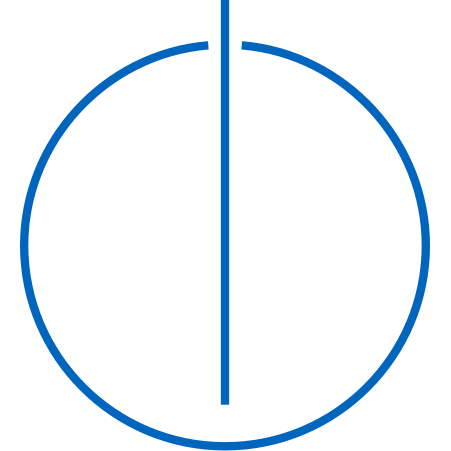
\includegraphics[height=20mm]{logos/faculty.png}
  }{}
\end{titlepage}


\frontmatter{}

%\begin{titlepage}
  \centering

  \IfFileExists{logos/tum.pdf}{%
    
\includegraphics[height=20mm]{logos/tum.pdf}
  }{%
    \vspace*{20mm}
  }

  \vspace{5mm}
  {\huge\MakeUppercase{\getFaculty{}}}\\

  \vspace{5mm}
  {\large\MakeUppercase{\getUniversity{}}}\\

  \vspace{20mm}
  {\Large \getDoctype{}}

  \makeatletter
  \vspace{15mm}
  \ifthenelse{\pdf@strcmp{\languagename}{english}=0}
  {
  {\huge\bfseries \getTitle{}}

  \vspace{10mm}
  {\huge\bfseries \foreignlanguage{ngerman}{\getTitleGer{}}}
  }
  {
  {\huge\bfseries \getTitleGer{}}

  \vspace{10mm}
  {\huge\bfseries \foreignlanguage{english}{\getTitle{}}}
  }
  \makeatother

  \vspace{15mm}
  \begin{tabular}{l l}
    Author:          & \getAuthor{} \\
    Supervisor:      & \getSupervisor{} \\
    Advisor:         & \getAdvisor{} \\
    Submission Date: & \getSubmissionDate{} \\
  \end{tabular}

  \IfFileExists{logos/faculty.png}{%
    \vfill{}
    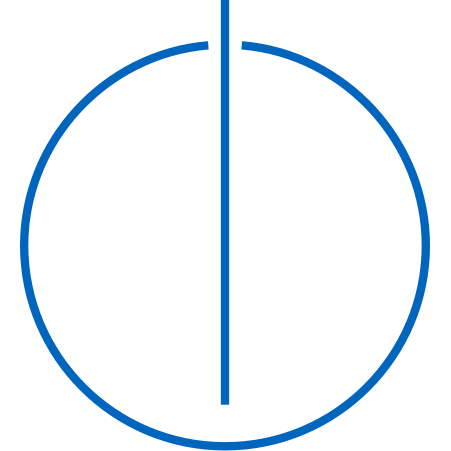
\includegraphics[height=18mm]{logos/faculty.png}
  }{}
\end{titlepage}

%\thispagestyle{empty}
\vspace*{0.8\textheight}
\noindent
\makeatletter
\ifthenelse{\pdf@strcmp{\languagename}{english}=0}
{I confirm that this \MakeLowercase{\getDoctype{}} is my own work and I have documented all sources and material used.}
{Ich versichere, dass ich diese \getDoctype{} selbstständig verfasst und nur die angegebenen Quellen und Hilfsmittel verwendet habe.}
\makeatother

\vspace{15mm}
\noindent
\getSubmissionLocation{}, \getSubmissionDate{} \hspace{50mm} \getAuthor{}

\cleardoublepage{}

%\makeatletter
\ifthenelse{\pdf@strcmp{\languagename}{english}=0}
{\addcontentsline{toc}{chapter}{Acknowledgments}}
{\addcontentsline{toc}{chapter}{Danksagungen}}
\makeatother
\thispagestyle{empty}

\vspace*{20mm}

\begin{center}
\makeatletter
\ifthenelse{\pdf@strcmp{\languagename}{english}=0}
{\usekomafont{section} Acknowledgments}
{\usekomafont{section} Danksagungen}
\makeatother
\end{center}

\vspace{10mm}

%TODO: Acknowledgments
I would like to say thanks to my research supervisor, Dr. rer. nat. Tim Steinhoff, for his continuous support, motivation and providing an excellent opportunity to write this thesis in GRS working on real industrial software.

\cleardoublepage{}

%\chapter{\abstractname}


\todo{reformulate the statement}
Parallel linear equation solvers are one of the most important components determining the scalability and efficiency of many supercomputing applications.\\

In many HPC applications, the optimized single-node performance is one of the most crucial building blocks for the optimization of probabilistic analysis or hybrid MPIOpenMP implementation.


%TODO: Abstract





%\nomenclature{MPI}{Message Passing Interface library}%
\nomenclature{PC}{Preconditioner}%
\nomenclature{n}{number of linear equations in a system}%
\nomenclature{nnz}{number of non-zeros in a matrix}%
%\nomenclature{$m$}{abc}

\printnomenclature


\microtypesetup{protrusion=false}
\tableofcontents{}
\microtypesetup{protrusion=true}

\mainmatter{}
\chapter{Introduction}\label{chapter:introduction}

% what is nuclear energy and why it is attractive?
Nowadays, nuclear energy is one of the main sources of electricity. It comes from splitting atoms in a reactor which, as a result, heats water up to the point where it is converted into pressurized steam. In its turn, the steam rotates turbines which, finally, produces electricity. According to the recent estimations, thermal efficiency of modern nuclear power plants lies in the range of 35-45\% which is comparable to conventional fossil fueled power plants \cite{intro:efficiency-of-nuclear-power-plants}. In spite of considerable initial investment,  nuclear power plants have low operating costs and longevity which makes them particularly cost effective.\\


% Advantages
In recent years, nuclear power plants have become attractive means of power generation because of relatively low emission of carbon dioxide. As a result, the green house gase emissions to the atmosphere and thus the contribution of nuclear power plants to global warming is relatively less \cite{intro:pros-and-cons-of-nuclear-power}.\\


% Example of nuclear energy utilization in the EU
Today, nuclear power plants generate almost 30\% of the electricity produced in the European Union (EU). There are almost 130 nuclear reactors in operation in 14 EU countries, namely: Belgium, Bulgaria, Czech Republic, Finland, France, Germany, Hungary, Netherlands, Romania, Slovakia, Slovenia, Spain, Sweden, and the United Kingdom \cite{intro:eu-nuclear-industry-general}.\\


% danger of nuclear power
% Disadvantages: Accidents Can Happen
% idea: requirements to perform hundreds of experiments and foresee all possible outcomes.
The main problem assosiated with nuclear power is radioactive waste which is extremely dangerous for people and environment and has to be carefully looked after for several thousand years after utilization. Any accident in a plant can lead to grave consequences at a scale similar to Chernobyl disaster. For this reason, nuclear safety is one of the most important topics in this area. It demands a huge amount of testing and analysis to be performed before and during operation of a nuclear power plant in order to predict any possiblity of unwanted outcomes and devise preventive measures against such accidents. The topic has become even more prominent after 2011 Fukushima accident. In response to the disaster, numerous stress tests were conducted to measure the ability of the EU nuclear industry to withstand any kind of natural disaster \cite{intro:eu-nuclear-industry-general}.\\



% 1. \gls{grs}: general info and the goal
% 2. Simulation tools
Since 1977, Gesellschaft für Anlagen- und Reaktorsicherheit (\gls{grs}) has been the main German scientific research institute in the field of nuclear safety and radioactive waste management \cite{grs:grs-general-info}. Today, the organization carries out advanced research and analysis in the field of reactor safety, radioactive waste management as well as radiation and environmental protection \cite{grs:grs-general-info}. Due to the inability to create various nuclear accident test scenarios, which by their very nature could be catastrophic, \gls{grs} develops and provides numerous simulation software products to cope with this problem. A short description of the main software packages developed by \gls{grs} is provided in table \ref{table:introduction-grs-software}.\\

%Due to a huge amount of testing, various types of possible accidents and disability to conduct natural experiments, \gls{grs} provides and develops numerous simulation software products to cope with this problem. Table \ref{table:introduction-grs-software} represents the main software packages that have been developed by \gls{grs} and their short description.\\

\begin{table}[htb]
\centering
\begin{tabular}{|c|l|}
\hline
Name          & \multicolumn{1}{c|}{Description}                                                                                                                                                             \\ \hline
ATHLET        & \begin{tabular}[c]{@{}l@{}}Thermohydraulic safety analyses for the primary\\ circuit of  LWRs\end{tabular}                                                                                   \\ \hline
ATHLET-CD     & \begin{tabular}[c]{@{}l@{}}Analyses of accidents with core meltdown \\ and fission product release for LWRs\end{tabular}                                                                     \\ \hline
ATLAS         & \begin{tabular}[c]{@{}l@{}}Analysis simulator for interactive handling \\ and  visualisation of several computer codes\end{tabular}                                                          \\ \hline
COCOSYS       & \begin{tabular}[c]{@{}l@{}}Analyses of severe incidents in the \\ containment of LWRs\end{tabular}                                                                                           \\ \hline
DORT/TORT     & \begin{tabular}[c]{@{}l@{}}Solution of time-dependant neutron transport\\ equations for 2D/3D transients analyses\end{tabular}                                                               \\ \hline
QUABOX/CUBBOX & 3-D neutron kinetics core model                                                                                                                                                              \\ \hline
SUSA          & Uncertainty and sensitivity analyses                                                                                                                                                         \\ \hline
TESPA-ROD     & Core rod code for design basis accidents                                                                                                                                                     \\ \hline
\end{tabular}
\caption{A list of software developed by \gls{grs}, \cite{grs:grs-general-info}}
\label{table:introduction-grs-software}
\end{table}



% objective of the study
The main focus of this study is dedicated to \gls{athlet} software package as well as its Numerical Toolkit. The goal of the study is to identify the most compute-intensive parts of the \gls{athlet}-\gls{nut} code and possibly accelerate its execution time.\\

step
\chapter{Overview of \gls{athlet} and \gls{nut} software}\label{chapter:athlet-nut}

\section{\gls{athlet}}
\label{sec:athlet-overview}


The thermal-hydraulic system code \acrshort{athlet} (Analysis of THermal-hydraulics of LEaks and Transients) is developed by \acrshort{grs} for the analysis of the whole spectrum of operational conditions, incidental transients, design-basis accidents and beyond design-basis accidents without core damage anticipated for nuclear energy facilities \cite{grs:athlet-info}. The code provides specific models and methods for the simulation of many types of nuclear power plants comprising current light water reactors (PWR\footnote{Pressurized Water Reactor}, BWR\footnote{Boiling Water Reactor}, WWER\footnote{Water-Water Energetic Reactor}, HPCR\footnote{High Power Channel-type Reactor}), advanced Generation III+ and IV reactors as well as SMRs\footnote{Small Modular Reactor} \cite{grs:athlet-info}.\\


Physical processes inside of hydraulic circuits of light-water reactors can be naturally described by a two-phase thermo-fluiddynamic model based on conservation equations of mass, momentum and energy for liquid and vapor.\\

1. Liquid mass
\begin{equation} \label{eq:athlet-1}
\frac{\partial ((1-\alpha)\rho_{l})}{\partial t} + \nabla ((1-\alpha) \rho_{l} \vec{w_{l}}) = - \psi
\end{equation}


2. Vapor mass
\begin{equation} \label{eq:athlet-2}
\frac{\partial (\alpha \rho_{v})}{\partial t} + \nabla (\alpha \rho_{v} \vec{w_{v}}) = \psi
\end{equation}


3. Liquid momentum
\begin{equation} \label{eq:athlet-3}
\frac{\partial ((1-\alpha) \rho_{l} \vec{w_{l}})}{\partial t} + \nabla ((1-\alpha) \rho_{l} \vec{w_{l}} \vec{w_{l}}) + \nabla ((1 - \alpha)p) = \vec{F_{l}}
\end{equation}


4. Vapor momentum
\begin{equation} \label{eq:athlet-4}
\frac{\partial (\alpha \rho_{v} \vec{w_{v}})}{\partial t} + \nabla (\alpha \rho_{v} \vec{w_{v}} \vec{w_{v}}) + \nabla (\alpha p) = \vec{F_{v}}
\end{equation}


5. Liquid energy
\begin{equation} \label{eq:athlet-5}
\frac{\partial \Big[ (1-\alpha)\rho_{l}(h_{l} + \frac{1}{2} \vec{w_{l}} \vec{w_{l}} - \frac{p}{\rho_{l}}) \Big]}{\partial t} + \nabla \Big[ (1-\alpha)\rho_{l}\vec{w_{l}}(h_{l} + \frac{1}{2} \vec{w_{l}} \vec{w_{l}}) \Big] = - p \frac{\partial (1 - \alpha)}{\partial t} + E_{l}
\end{equation}


6. Vapor energy
\begin{equation} \label{eq:athlet-6}
\frac{\partial \Big[ \alpha \rho_{v}(h_{v} + \frac{1}{2} \vec{w_{v}} \vec{w_{v}} - \frac{p}{\rho_{v}}) \Big]}{\partial t} + \nabla \Big[ \alpha\rho_{v}\vec{w_{v}}(h_{v} + \frac{1}{2} \vec{w_{v}} \vec{w_{v}}) \Big] = - p \frac{\partial \alpha}{\partial t} + E_{v}
\end{equation}

7. Volume vapor fraction
\begin{equation} \label{eq:athlet-7}
	\alpha = \frac{V_{v}}{V}
\end{equation}


where $p$ - pressure of mixture, $\psi$ - mass source term, $\vec{F}$ - external composite force acted on a control volume, $E$ - external composite energy source term within a control volume, subscripts $l$ and $v$ denote liquid and vapor phases, respectively. \\


% Finite volume and 1D discritiazation 
Spacial integration of the conservation equations, the ssystem \ref{eq:athlet-1} - \ref{eq:athlet-7}, is performed on the basis of finite-volume method with using one dimensional formulation, figure \ref{fig:introduction-1d-fvm}.


\figpointer{\ref{fig:introduction-1d-fvm}}
\begin{figure}[htpb]
  \centering
  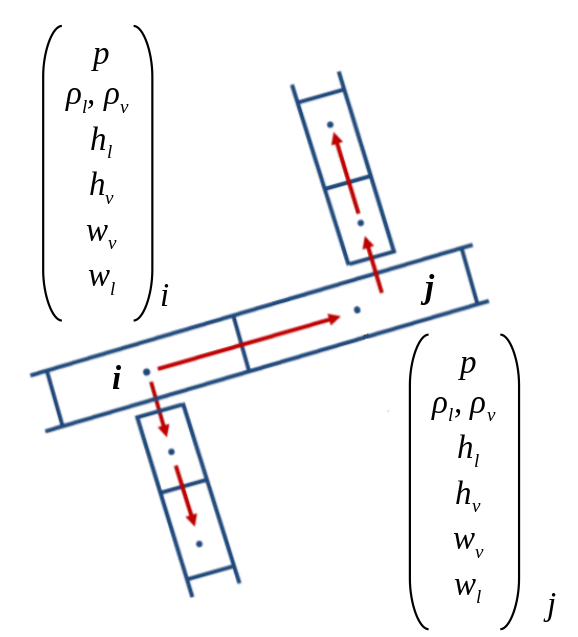
\includegraphics[width=0.55\textwidth]{figures/introduction-1d-fvm.png}
\caption{One dimensional finite volume formulation of thermo-hydraulic modeling in \acrshort{athlet}, \cite{tims-presentation}}
\label{fig:introduction-1d-fvm}
\end{figure}


Finally, the system is transformed to a non-autonomous system of ordinary differential equations and expressed as an initial value problem, equation \ref{eq:athlet-8}, after spatial finite-volume integration and many mathematical transformations \cite{lt:ATHLMaM}. 


\begin{equation} \label{eq:athlet-8}
	\frac{dy}{dt} = f(t,y), \;  t_{0} \leq t \leq t_{F} \; y(t_{0}) = y_{0}
\end{equation}

where $y \in \mathbb{R}^{N}$ is a composite vector of variables, $f$ is a non-linear function such that $f : \mathbb{R} \times \mathbb{R}^{N} \supset \Omega  \rightarrow \mathbb{R}^{N}$  .\\


% Rosenbrock-Wanner
Analysis of system \ref{eq:athlet-8} shows the problem is rather and thus must to be solved with an implicit solver. Rosenbrock methods are a class of linear implicit methods which is capable of solving such stiff systems of \acrshort{ode}s efficiently. The methods replace non-linear systems with a sequence of linear ones, however, some stability and accuracy properties are usually lost \cite{blom2013rosenbrock}. An additional drawback of the methods is evaluation of the exact Jacobian at every time step which affects computational cost.\\


To decrease the cost and preserve sufficient accuracy of numerical integration, \acrshort{athlet}, instead, uses a W-method of the third order. W-methods belong to the family of Rosenbrock methods, however, calculate the Jacobian matrix occasionally. The \acrshort{athlet} developers spent much of their time and efforts to develop heuristics to identify instances of time when evaluation of the Jacobian must be performed. In other words, the algorithm can re-use the same Jacobian matrix approximation between steps with some partial matrix updates. However, when a hydraulic circuit state drastically changes due to transitivity, the evaluation of the full Jacobian is demanded.\\


\figpointer{\ref{fig:introduction-w-method-scheme}}
\begin{figure}[htpb]
  \centering
  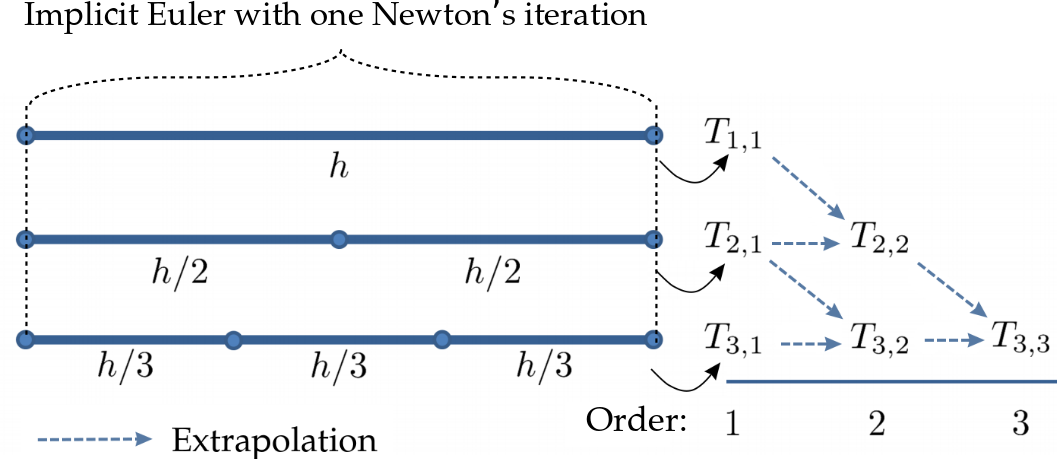
\includegraphics[width=0.8\textwidth]{figures/introduction-rosenbrock-scheme.png}
\caption{A general view on the 6-stage W-method implemented in \acrshort{athlet}}
\label{fig:introduction-w-method-scheme}
\end{figure}


In the general case, a step of the W-method method, implemented in \acrshort{athlet}, can be viewed as a sequence of six stages in the following way. Each stage uses implicit Euler method and exactly one Newton's iteration to evaluate the value of vector $y$ at the next integration step $h$ with different accuracy. Then, the obtained values are extrapolated, in order explained in figure \ref{fig:introduction-w-method-scheme}, to achieve desired order of integration. By and large, the algorithm can be expressed in a compact form of equation \ref{eq:athlet-9}.

\begin{equation} \label{eq:athlet-9}
	((h \gamma)^{-1}I - J) \Delta z^{l}_{i} = - h^{-1} z^{l}_{i} + f(t_0 + \tau_{i} h, y_{0} + z^{l}_{i})
\end{equation}

where $\Delta z^{l}_{i} = z^{l+1}_{i} - z^{l}_{i}$, $z^{l}_{i} = y^{l}_{i} - y^{l}_{i - 1}$, $J \approx \frac{\partial f}{\partial y}$ - approximation of Jacobian matrix, $l = 1,2$ - Newton's iteration index, $i = 1, 2, 3$ - integration step index.\\


\section{\acrshort{nut}}

Numerical Toolkit, or just \acrshort{nut}, can be viewed as a container of various dense and sparse linear algebra subroutines which can run in parallel on distributed-memory machines. \acrshort{nut} design follows the paradigm of \textit{Adapter/Wrapper} pattern which provides a uniform common interface for its services to various \acrshort{grs} simulation tools (outlined in table \ref{table:introduction-grs-software}) and thus helps to achieve re-usability, flexibility and extensibility properties of the code.\\


Currently, \acrshort{nut} is based heavily on Portable, Extensible Toolkit for Scientific Computation, known as \acrshort{petsc} library. It is one of the most widely used parallel numerical software  library \cite{wiki:petsc-general-info}. It includes a large suite of parallel linear and nonlinear equation solvers as well as its software-infrastructure to handle computations on distributed-memory machines by means of Message Passing Interface (\acrshort{mpi}) and specific data structures. Fortunately, though a careful selection of the design pattern, \acrshort{nut} can be easily extended to provide an extra service or an external library access which has not been implemented in \acrshort{petsc} yet.\\ 


\section{\acrshort{athlet}-\acrshort{nut} coupling}
\label{sec:athlet-nut-coupling}

\figpointer{\ref{fig:introduction-nut-process-groups}}
\begin{figure}[htpb]
  \centering
  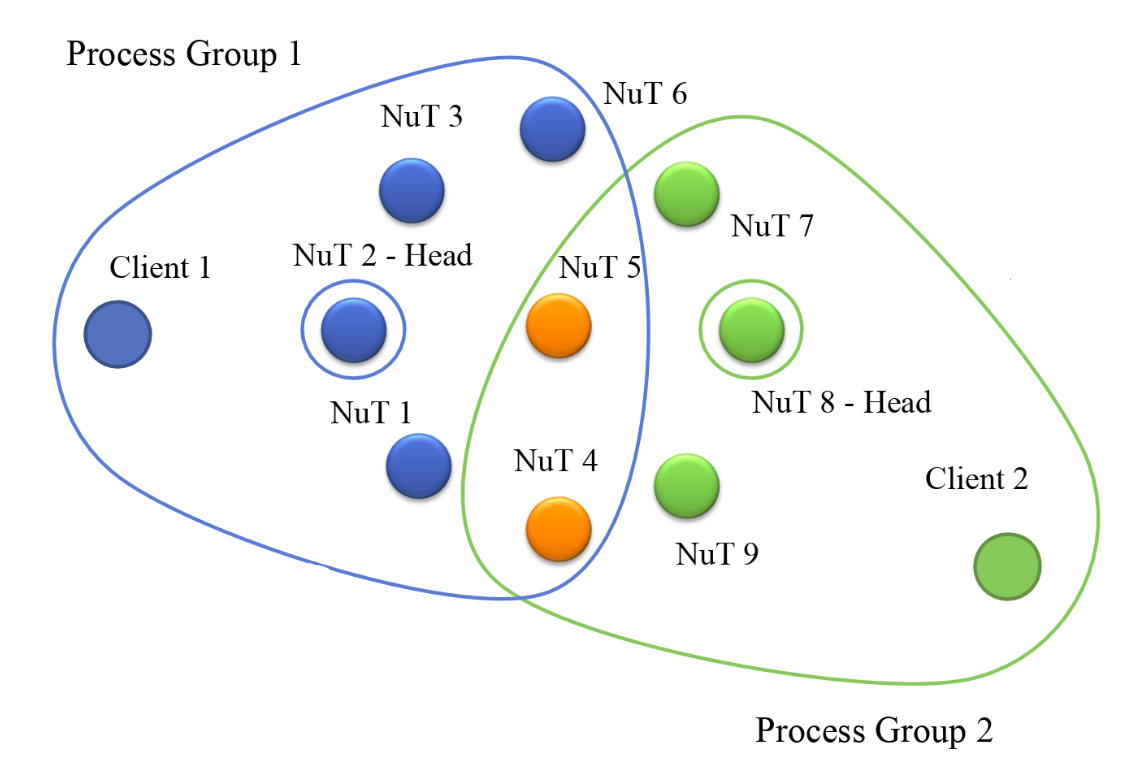
\includegraphics[width=0.8\textwidth]{figures/introduction-nut-process-groups.png}
\caption{An example of \acrshort{nut} process groups}
\label{fig:introduction-nut-process-groups}
\end{figure}

Coupling of \acrshort{nut} with \acrshort{grs} tools is based on the client-server architecture where \acrshort{nut} acts as a server and the tools can be viewed as clients. Communication between two parts is done via \acrshort{mpi}.\\


To provide a clear and concise external interface, \acrshort{nut} contains a client module called "\acrshort{nut} Plug-in". It can be  considered as a socket, from the client side, using the analogy of Transmission Control Protocol (TCP). The plug-in hides all \acrshort{mpi} calls to the sever which considerably improves readability of the code.\\


% communicators
In the general case, \acrshort{nut} allows multiple clients to work concurrently with the server. To handle the traffic, the library splits the default \acrshort{mpi} communicator at start-up time of the application into appropriate process groups, as it is shown in figure \ref{fig:introduction-nut-process-groups}.\\



The design of \acrshort{nut} allows sharing of some \acrshort{nut}-\acrshort{mpi} processes among different process groups due to performance reasons i.e. finite number of processing units on hardware. To resolve possible deadlocks, each process group has its own representative, called the head. Each client has two views on its respective group which is achieved by means of distinct \acrshort{mpi} communicators. The first communicator is responsible for client-head communication whereas the second one allows the client to talk to any \acrshort{nut} process within the group.\\



A general view of client-server communication looks like a 3-way handshake in the following way: a client sends a request to the head which is a signal to reserve all compute-units of the group for an upcoming task. Having possessed the resources and prepared them for a specific service, the head notifies the client about resource acquisition and the entire process group waits for data. Afterwards, the client sends data either to a specific \acrshort{nut}-process or to the entire group using the second communicator and waits for a result of the service. In the current implementation of \acrshort{nut}, the communication between client and server is synchronous i.e. the client gets blocked while waiting for a result from the server. \\


As an example, figure \ref{fig:introduction-athlet-nut-coupling} represents a general view of \acrshort{athlet}-\acrshort{nut} coupling where \acrshort{athlet} is responsible for marching of the numerical integration solver whereas \acrshort{nut} computes solutions of systems \ref{eq:athlet-9}.\\


\figpointer{\ref{fig:introduction-athlet-nut-coupling}}
\begin{figure}
  \centering
  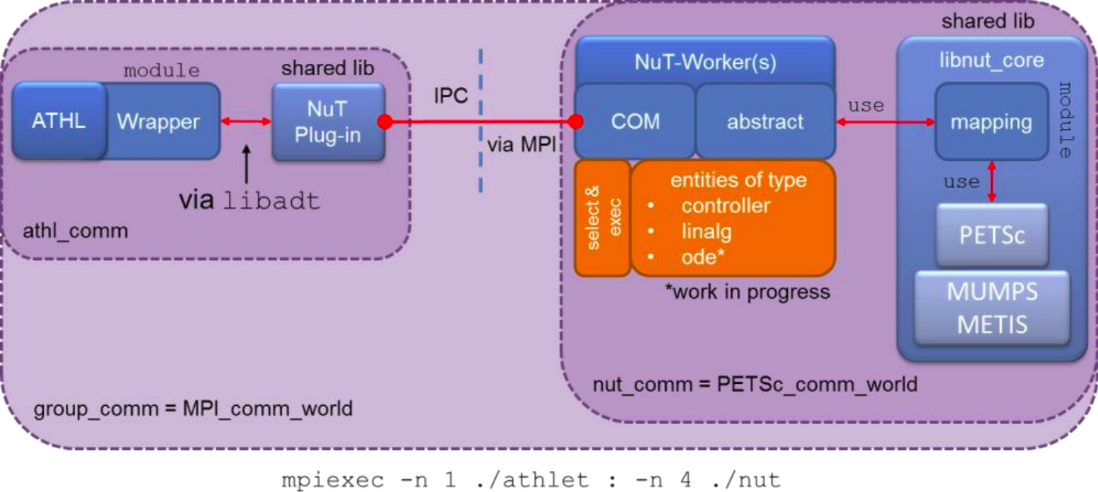
\includegraphics[width=0.75\textwidth]{figures/introduction-athlet-nut-coupling.png}
    \caption{\acrshort{athlet}-\acrshort{nut} software coupling}
\label{fig:introduction-athlet-nut-coupling}
\end{figure}


Partial and full Jacobian matrix updates derived from finite differences are computed on the client side since only the client has the access to function $f(y)$, equation \ref{eq:athlet-8}. Due to decoupling of the underlying system of \acrshort{pde}s and specifics of finite volume discretization, Jacobian matrix is rather sparse and, therefore, \acrshort{athlet} uses a Jacobian matrix compression algorithm, described in section \ref{sec:jacobian-matrix-compression}, to reduce the amount of Jacobian column evaluations. Having computed a matrix column, \acrshort{athlet} immediately broadcasts it to its entire \acrshort{nut} process group by means of 3-way handshake mechanism as described above. It is worth mentioning that this approach allows to circumvent potential memory limits on the client side and thus store the entire sparse Jacobian matrix in a distributed fashion on the server. In other words, \acrshort{athlet} never holds the entire Jacobian matrix in its memory; conversely, the matrix is distributed across multiple \acrshort{nut} processes according to block-row distribution induced by \acrshort{petsc}. In turn, \acrshort{nut} is waiting for the entire Jacobian matrix information from \acrshort{athlet} and starts solving systems \ref{eq:athlet-9} right after the corresponding request from the client.\\



\chapter{Problem Statement}\label{chapter:problem-statment}


Integration of a system of \acrshort{ode}s by means of W-methods can be considered as solutions of a sequence of linear systems from another point of view. Equations \ref{eq:athlet-9} can be rewritten in a form \ref{eq:athlet-10}, after grouping both the right- and left-hand sides in a single matrix and vector, respectively.\\


%\begin{equation} \label{eq:athlet-10}
%	A_{i} \Delta z^{l}_{i} =  b^{l}_{i} 
%\end{equation}

\begin{equation} \label{eq:athlet-10}
	A_{i} \delta y_{ij} =  b_{ij} 
\end{equation}


where $A = (I - h_{i}J)$  is a $\mathbb{R}^{N} \times \mathbb{R}^{N}$ nonsingular sparse matrix; $\delta y_{ij}$  and $b_{ij}$ are $\mathbb{R}^{N}$ vectors.\\


According to the integration scheme, figure \ref{fig:introduction-w-method-scheme}, and definition of the method, each step of numerical integration requires to solve 6 linear systems with 3 distinct matrices, resulting from the Jacobian matrix by the corresponding shifts of the main diagonal. Therefore, the computational burden of the W-method mainly lies in solving sparse linear systems.\\


There exist two families of linear sparse solvers, namely: iterative and direct sparse methods. In the general case, execution time of any method, regardless of a solver family, is bounded by $O(n^2)$ complexity due to matrix sparsity, where $n$ is number of equations in a system. However, a constant in front of the factor $n^2$ can vary significantly between the methods which explains differences in execution time. Additionally, it is important to mention the families use absolutely different approaches for solving sparse linear systems and thus posses different numerical properties. Among all  properties, there are some which are particularly important for efficient execution of W-methods, namely: \\


\begin{itemize}
	\item robustness of a methods to treat, in particular, ill-conditioned systems
	\item parallel efficiency
\end{itemize}


These above mentioned properties can be treated as non-functional requirements to a sparse linear solver for efficient numerical time integration.\\

 
Finding solutions of sparse linear systems is a well-known and commonly occurring problem in the field of scientific computing and, therefore, numerous implementations of different kinds of linear solvers exist. However, the \acrshort{nut} project imposes some extra constrains due to the design philosophy adopted by \acrshort{grs}: \\


\begin{itemize}
	\item open-source license
	\item direct interface to \acrshort{petsc}
\end{itemize}

%In particular, it requires a particular solver implementation to have its \textbf{open-source license} and to have its direct \textbf{interface to \acrshort{petsc}} library.\\


In this study, we are primarily concerned with a selection and configuration of a  sparse linear solver which can cover all requirements listed above.\\


This report is organized as follows. Chapter \ref{subseq:matrix-sets-and-hardware} provides information about methodology, data, software and hardware used in this study. Subsections \ref{subseq:iterative-theory} and \ref{subseq:direct-sparse methods} give an overview of the theory and parallelization aspects of iterative and sparse direct methods. Then, in subsection \ref{subseq:hybrid-method-description}, we make a conclusion about which type of sparse linear methods is the best suited for numerical time integration governed by W-methods. In subsection 
\ref{subseq:mm-library-choice}, a particular implementation of a specific method is selected by means of testing. From chapter \ref{mumps:solver-configuration} onwards, we perform configuration and adaptation of a solver for distributed-memory computations. At the end, subsection \ref{subseq:mm-conclusion} summarizes obtained results and makes a general conclusion with respect to data and compute environment provided by  \acrshort{grs}.\\




An additional topic, considered in this study, is an improvement of \acrshort{athlet}-\acrshort{nut} communication during Jacobian matrix transfers. As it was described in subsection \ref{sec:athlet-nut-coupling}, \acrshort{athlet}, the client, transfers a Jacobian matrix in a column-wise fashion. \acrshort{nut}, the server, treats each column transfer as a service and, therefore, each transfer passes through the 3-way handshake described in subsection \ref{sec:athlet-nut-coupling}. Moreover, it is important to mention one more time,   due to the current implementation of \acrshort{athlet}-\acrshort{nut} coupling, client-server communication is blocking. In other words, \acrshort{athlet} gets blocked till completion of a column transfer. \\


The main goal of Jacobian matrix compression, described in section \ref{sec:jacobian-matrix-compression}, is to minimize the number of perturbations of non-linear function $f(y)$, equation \ref{eq:athlet-8}. Additionally it allows to reduce an amount of column transfers as well. Therefore, it improves the overall application performance from both computational and communication points of view. However, there are still some aspects to be considered.\\


Due to specifics of the matrix compression algorithm, described in section \ref{sec:jacobian-matrix-compression}, column lengths are decreasing between the first and last columns of a compressed Jacobian matrix form which, as a result, leads to unequal \acrshort{mpi} message sizes.\\


In this part of the study, we introduce a concept called \textit{accumulator} which allows to transfer a compressed Jacobian matrix in equal chunks. This approach potentially solves three important problems at once. First of all, \textit{accumulator} can help to get rid of small \acrshort{mpi} messages and thus improves network bandwidth utilization. Secondly, it helps to reduce an amount of synchronizations between the client and server and, therefore, improves operation of \acrshort{nut} as the server. Lastly, it allows to apply non-blocking \acrshort{mpi} communication on the client side and thus overlap Jacobian matrix transfers with computations.\\


In section \ref{sec:jacobian-matrix-compression}, we briefly describe the Jacobian matrix compression algorithm and the resulting \acrshort{athlet}-\acrshort{nut} communication problem. In section \ref{sec:accumulator-approach}, we present and describe the algorithm which is supposed to resolve the problem. Section \ref{sec:benchmark-and-test-data} provides a description of developed benchmarks and test data. Then, we focus and explain obtained results in section \ref{sec:accumulator-results}. Finally, in section \ref{sec:accumulator-conclusions}, we provide a general conclusion of the performed part of the study and summarize the results.\\

%\chapter{Methodology and Experimental Setup}\label{subseq:matrix-sets-and-hardware}

%Static solver configuration
\acrshort{athlet} is a tool designed for computer-based simulations of transient thermo-hydraulic problems where topology of hydraulic circuits can be changed during a numerical simulation. As a result, the Jacobian matrix often changes with respect to both numerical values and the matrix sparsity structure between integration time steps. Hence, a configuration of a linear solver in run-time becomes a time consuming and compute-expensive problem since \acrshort{athlet} usually generates hundreds of matrices during a simulation. Moreover, results of such dynamic solver configurations may be difficult to analyze and interpret.\\


In this study, it was decided to stick to a so-called static solver configuration approach: configuring a solver with only a small set of matrices, i.e. GRS matrix set, randomly saved during simulations of the most common \acrshort{grs} test scenarios. In the general case, this approach may lead to not accurate conclusions, however, it is only one feasible.\\


Besides \acrshort{grs} matrix set, the second set was  used for verification purposes of testing results. The set, called SuiteSparse matrix set, was generated by donwloading a dozen of matrices from SuiteSparse Matrix Collection \cite{sparse-matrix-collection:1}, \cite{sparse-matrix-collection:2} where we tried to pick out different matrices with respect to both the number of equations $n$ and matrix density i.e. ratio between the number of non-zero elements $nnz$ and the number of equations in a system.\\ 


The main matrix properties as well as matrix sparsity patterns are shown in tables \ref{table:grs-matrix-set}, \ref{table:suite-sparse-matrix-set} and appendix \ref{app:sparsity-patterns}.\\


\begin{table}[ht]
\small
\centering
\begin{tabular}{|c|c|c|c|c|c|}
\hline
Name     & \textit{n}       & \textit{nnz}      & \textit{nnz} / \textit{n} & \begin{tabular}[c]{@{}c@{}}Approximate\\ Condition\\  Number\end{tabular} & Structure     \\ \hline
pwr-3d   & 6009    & 32537    & 5.4147  & 1.019e+07                                                                 & SYMM-PTRN \\ \hline
cube-5   & 9325    & 117897   & 12.6431 & 1.592e+09                                                                 & SYMM-PTRN \\ \hline
cube-64  & 100657  & 1388993  & 13.7993 & 7.406e+08                                                                 & SYMM-PTRN \\ \hline
cube-645 & 1000045 & 13906057 & 13.9054 & 6.474e+08                                                                 & SYMM-PTRN \\ \hline
k3-2     & 130101  & 787997   & 6.0568  & 1.965e+15                                                                 & SYMM-PTRN \\ \hline
k3-18    & 1155955 & 7204723  & 6.2327  & 1.947e+12                                                                 & SYMM-PTRN \\ \hline
\end{tabular}
\caption{\acrshort{grs} matrix set \textit{(where SYMM - symmetric; NON-SYMM - non-symmetric; SYMM-PTRN- non-symmetric but with symmetric sparsity pattern)}}
\label{table:grs-matrix-set}
\end{table}




\begin{table}[ht]
\centering
\small
\begin{tabular}{|c|c|c|c|c|c|c|}
\hline
Name        & \textit{n}       & \textit{nnz}      & \textit{nnz} / \textit{n} & \begin{tabular}[c]{@{}c@{}}Approximate\\ Condition\\ Number\end{tabular} & Structure & Problem                                                      \\ \hline
cant        & 62451   & 4007383  & 64.1684 & 5.082e+05 & SYMM      & -                                                            \\ \hline
consph      & 83334   & 6010480  & 72.1251 & 2.438e+05 & SYMM      & -                                                            \\ \hline
CurlCurl\_3 & 1219574 & 13544618 & 11.1060 & 2.105e+05                                                                & SYMM      & \begin{tabular}[c]{@{}c@{}}Model\\ Reduction\end{tabular}    \\ \hline
Geo\_1438   & 1437960 & 63156690 & 43.9210 & 4.677e+05                                                                 & SYMM      & -                                                            \\ \hline
memchip     & 2707524 & 13343948 & 4.9285  & 1.305e+07                                                                & NON\_SYMM & \begin{tabular}[c]{@{}c@{}}Circuit\\ Simulation\end{tabular} \\ \hline
PFlow\_742  & 742793  & 37138461 & 49.9984 & 5.553e+06                                                                & SYMM      & -                                                            \\ \hline
pkustk10    & 80676   & 4308984  & 53.4110 & 5.589e+02 & SYMM      & Structural                                                   \\ \hline
torso3      & 259156  & 4429042  & 7.0903  & 2.456e+03                                                                      & NON\_SYMM & -                                                            \\ \hline
x104        & 108384  & 8713602  & 80.3956 & 3.124e+05 & SYMM      & Structural                                                   \\ \hline
\end{tabular}
\caption{SuiteSparse matrix set \textit{(where SYMM - symmetric; NON-SYMM - non-symmetric; SYMM-PTRN- non-symmetric but with symmetric sparsity pattern)}}
\label{table:suite-sparse-matrix-set}
\end{table}

Approximations of condition numbers, shown in tables \ref{table:grs-matrix-set} and \ref{table:suite-sparse-matrix-set},  were computed using Rayleigh–Ritz procedure \cite{rayleigh-ritz-procedure}. \acrshort{gmres} solver configured with $1000$ iteration steps before the restart was applied to un-preconditioned systems to generate a Krylov subspace for each matrix. Then, the resulting Hessenberg matrices were used for approximating eigenspaces and the corresponding eigenvalues. The approximations should be treated as lower bounds since the algorithm overestimates the smallest eigenvalues.\\


%The objective of this study is to find and configure a sparse linear solver which can fulfill all requirements listed above for the \acrshort{grs} matrix set. It is worth pointing out, as it was mentioned in section \ref{sec:athlet-overview}, \acrshort{athlet} performs many mathematical transformations upon the original system and, finally, generates an approximation of a Jacobian matrix. For that reason, one can assume that \acrshort{grs} matrix set can be structurally different from matrices coming naturally from finite-volume, finite-elements discretization or optimization problems. Therefore, SuiteSparse matrix set was used, from time to time, to examine this statement.\\


Two different hardware were available for this study. The first machine was a compute-cluster installed in \acrshort{grs} (\gls{hw1}) which was the main target. Additionally, \acrshort{lrz} CoolMUC-2 Linux cluster (\gls{hw2}) was used every time when some ambiguous results were obtained in order to check whether a problem was hardware, software or algorithmic specific. Table \ref{table:hardware-spec} shows compute-node specifications of both compute-clusters.\\


\begin{table}
\centering
\small
\begin{tabular}{|l|c|c|}
\hline
                    & HW1 (GRS) & HW2 (LRZ Linux) \\ \hline
Architecture        & x86\_64 & x86\_64 \\ \hline
CPU(s)              & 20 &  28 \\ \hline
On-line CPU(s) list & 0-19 &  0-27 \\ \hline
Thread(s) per core  & 1 &  1 \\  \hline
Core(s) per socket  & 10 & 14 \\ \hline
Socket(s)           & 2 &  2 \\ \hline
NUMA node(s)        & 2 &  4 \\ \hline
Model               & 62 &  63 \\ \hline
Model name          & E5-2680 v2 & 
E5-2697 v3 \\ \hline
Stepping            & 4 &  2 \\ \hline
CPU MHz             & 1200.0 &  2036.707 \\ \hline
Virtualization      & VT-x &  VT-x \\ \hline
L1d cache           & 32K &  32K \\ \hline
L1i cache           & 32K &  32K \\ \hline
L2 cache            & 256K &  256K \\ \hline
L3 cache            & 25600K &  17920K \\ \hline
NUMA node0 CPU(s)   & 0-9 &  0-6 \\ \hline
NUMA node1 CPU(s)   & 10-19 &  7-13 \\ \hline
NUMA node2 CPU(s)   & - &  14-20 \\ \hline
NUMA node3 CPU(s)   & - &  21-27 \\ \hline
RAM per node, GB   & 128 &  64 \\ \hline
\end{tabular}
\caption{Hardware specification}
\label{table:hardware-spec}
\end{table}


For this study, OpenMPI implementation of the \acrshort{mpi} standard was used because of its open-source license and comprehensive documentation. The library has many options for processes pinning which was intensively used during the study.\\


To make process pinning explicit and deterministic, a python script was developed to generate rank-files automatically based on the number of \acrshort{mpi} processes, \acrshort{openmp} threads per \acrshort{mpi} process, the maximum number of processing elements and the number of \acrshort{numa} domains. The scrip always leaves appropriate gaps between \acrshort{mpi} processes to allow each process to fork the corresponding number of threads within a parallel region.\\


\begin{figure}[h!]
\centering
	\begin{tabular}{cc}
			\subfloat[\textit{Spread} mode]{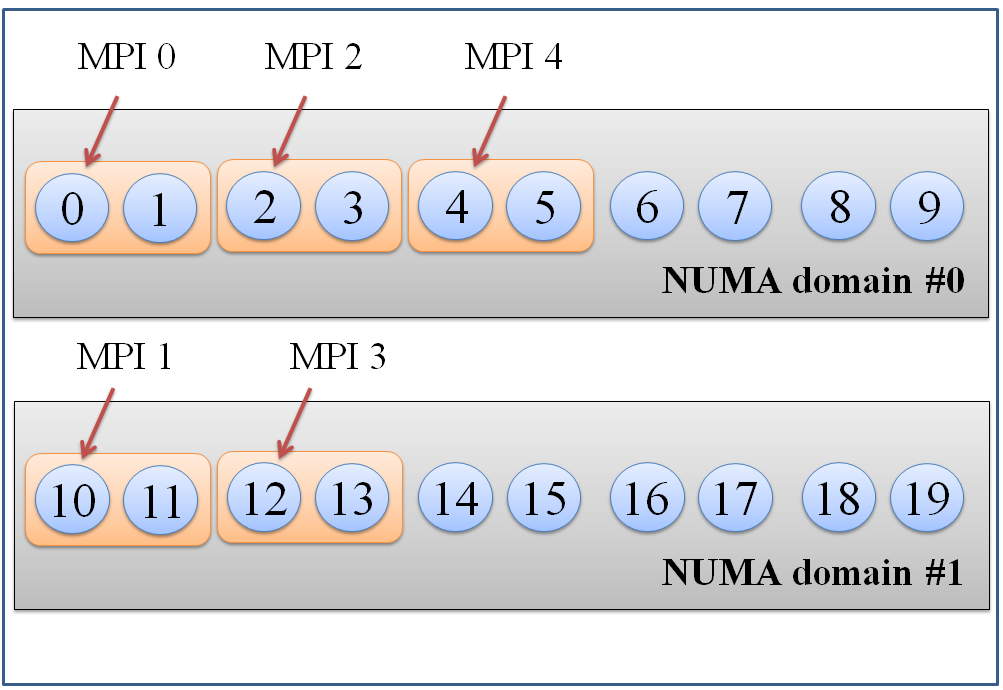
\includegraphics[width=0.45\textwidth]{figures/chapter-2/spread-mode.png}} &
		\subfloat[\textit{Close} mode]{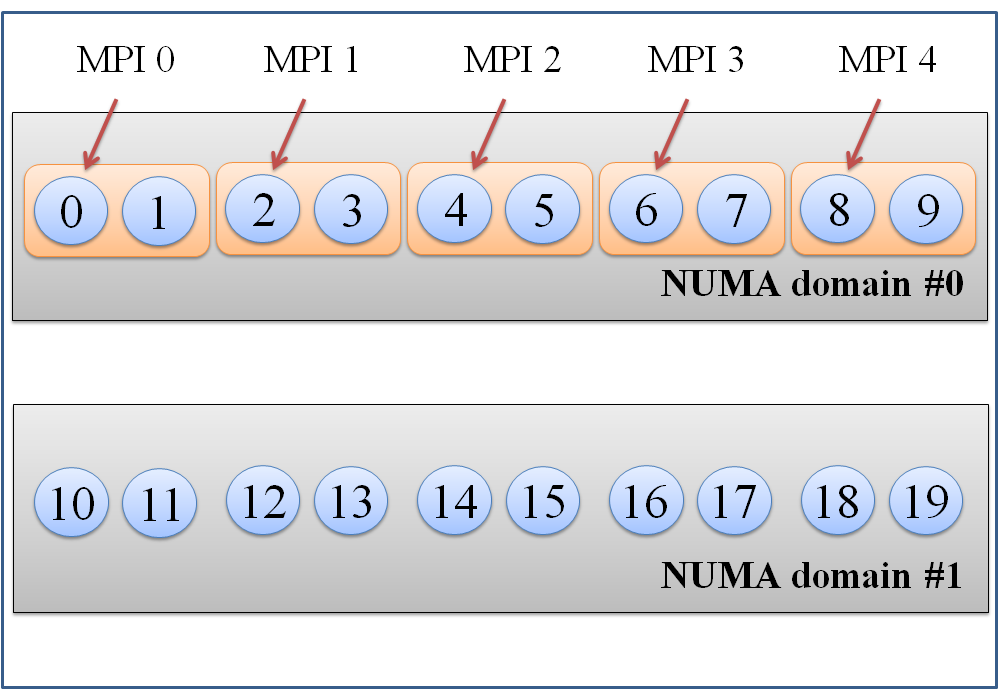
\includegraphics[width=0.45\textwidth]{figures/chapter-2/close-mode.png}} \\
	\end{tabular}
	\caption{An example of pinning 5 \acrshort{mpi} processes with 2 \acrshort{openmp} threads per process in case of \gls{hw1} hardware}
	\label{fig:python-script-rankfile-example}
\end{figure}


A rank-file specifies explicit mapping between \acrshort{mpi} processes, ranks, and actual processing elements, cores, of a machine. The script has two modes, namely: \textit{spread} and \textit{close}. Given a certain number of ranks, \textit{spread} mode tries to distribute them as spread as possible across multiple available \acrshort{numa} domains in a round-robin fashion. In contrast to \textit{spread} strategy, \textit{close} one groups ranks as close as possible to keep the maximum number of ranks within a single \acrshort{numa} domain. Figure \ref{fig:python-script-rankfile-example} shows an example of mapping 5 \acrshort{mpi} ranks and 2 \acrshort{openmp} threads per rank onto a compute node equipped with 20 cores and 2 \acrshort{numa} domains (\gls{hw1}).\\


In this study, \acrshort{petsc} 3.10 and OpenMPI 3.1.1 libraries were chosen and compiled with Intel 18.2 compiler.\\

%%\chapter{Theoretical and parallelization aspects of iterative and direct sparse methods}

\chapter{Overview of Sparse Linear Solver Types}\label{subseq:overview-of-linear-solver-types}

\section{Iterative Methods}
\section{Iterative methods}
\label{subseq:iterative methods}
Iterative methods, especially Krylov subspace methods that we are going to discuss in this section, are well known for their relatively low storage requirements $O(nnz)$ and computation cost $O(N^2)$ in case of sparse linear systems of equations and good condition number. It turns out that sometimes it might be only one way to solve huge systems with millions unknowns.\\

The most well known methods are Conjugate Gradient (CG) for symmetric positive definite matrices, Minimal Residual Method (MINRES) for symmetric indefinite systems, Generalized Minimal Residual Method (GMRES) for non-symmetric systems of linear equations as well as different variants of GMRES such Biconjugate Gradient Method (BiCG), Biconjugate Gradient Stabilized Method (BiCGSTAB) and so on.\\

All Krylov methods solve a system of equation as a minimization problem. For example, the goal of CG algorithm is to minimize the energy functional $f(x) = 0.5 x^T A x - b^T x + c$, whereas, MINRES and GMRES tries to minimize residual norm $r_{j}$ for $x_{j}$ in a subspace. \\

%$j$th Krylov subspace $\mathcal{K}_{j}$. \\

The methods construct an approximate solution of a system as a linear combination of vectors $b$, $Ab$, $A^2b$, $A^3b$ and so on which defines the Krylov subspace. At each iteration we expand the subspace adding and evaluating a next vector in the combination.\\

Let's consider GMRES, as the most popular and general iterative solver, without preconditioning to just analyze its strong scaling behavior and potential problems. \\ 

As we mentioned above GMRES minimizes the residual norm in a subspace $U_m$.

\begin{equation} \label{eq:Gmres-1}
	\underset{x \in U_m}{min}||Ax - b||^2
\end{equation}

We can consider a solution vector $x$ in the subspace $U_m$ in a form $x=U_m y$. Thus, equation \ref{eq:Gmres-1} can be written as following:

\begin{equation} \label{eq:Gmres-2}
	\underset{x \in U_m}{min}||AU_m y - b||^2
\end{equation}

The most natural way to choose a proper subspace $U_m$ is the corresponding Krylov subspace $\mathcal{K}_m$ because it can be easily generated on the fly. However, decomposition of vector $x$ in that subspace can be a problem. Since the subspace $\mathcal{K}_m$ is spanned by the sequence of $b$, $Ab$, $A^2b$, ..., $A^{m-1}b$ and due to round-off error the sequence can become linear dependent. Therefore, we have to compute and use the orthonormal base of the given Krylov subspace. Saad and Schultz in their work \cite{sparse-la:gmrese-origin} used Arnoldi process for constructing an $l_2$-orthogonal basis. As the results equation \ref{eq:Gmres-2} can be written in the following form:  \\

\begin{equation} \label{eq:Gmres-3}
	\underset{x \in U_m}{min}||U_{m+1}H_{m+1,m} y - ||b||u_1||^2 = \\
	\underset{x \in U_m}{min}||H_{m+1,m} y - ||b||e_1||^2 
\end{equation}

where $H_m$ is an upper Hessenberg matrix. We can apply Givens rotation algorithm to compute $QR$ decomposition to convert $H_m$ to a strictly upper triangular matrix. Thus,

 
\begin{equation} \label{eq:Gmres-4}
	\underset{x \in K_m}{min}||Ax - b||^2 = \\
	\underset{x \in U_m}{min}||Q^TRy - ||b||e_1||^2 = \\
	\underset{x \in U_m}{min}||\Big(\begin{array}{c c}R_m \\ 0 \\\end{array}\Big) y - \Big(\begin{array}{c c} \tilde{b_m} \\ \tilde{b_{n-m}} \\\end{array}\Big)||^2
\end{equation}

Given \ref{eq:Gmres-4}, we can compute the solution as following:

\begin{equation} \label{eq:Gmres-5}
	R_m y = \tilde{b_m}
\end{equation}


\begin{equation} \label{eq:Gmres-6}
	x_m = U_m y  
\end{equation}

Because of large computational and storage costs, in case of evaluation of the full Krylov subspace, only small a subspace is computed, typically first 20 - 50 column vectors. Then the algorithm is restarted using the computed approximate solution as a initial guess for the next iteration.\\

We can see that some operations, for example \ref{eq:Gmres-6}, can be efficiently done in parallel. However, operatiopns like sparse triangular solve \ref{eq:Gmres-5} can introduce some effect on strong scaling behavior. Figure \ref{fig:sparse-triangular-solve-performance} shows strong scaling performance results of a sparse parallel triangular solver with a two dimensional matrix distribution. Performance considerations of the solver can be found in \cite{sparse-la:triangular-solve}.\\

\figpointer{\ref{fig:sparse-triangular-solve-performance}}

\begin{figure}[htpb]
  \centering
  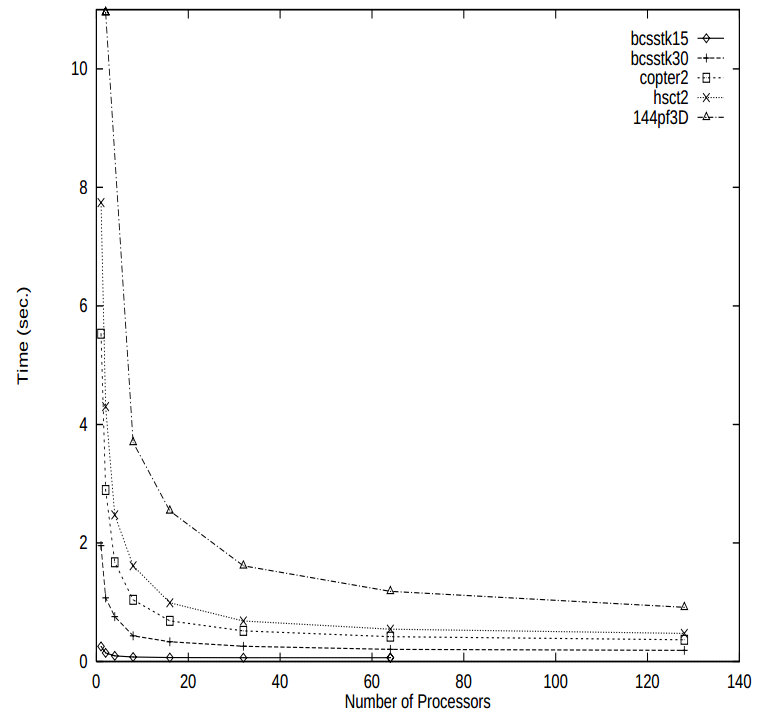
\includegraphics[width=0.5\textwidth]{figures/chapter-2/sparse-triangular-solve-performance.png}
\caption{Performance of sparse triangular solve \cite{sparse-la:triangular-solve}}
\label{fig:sparse-triangular-solve-performance}
\end{figure}


It is interesting to notice that performance of the triangular solver depends on a matrix sparsity structure as well as the matrix size. \\

Triangular solve \ref{eq:Gmres-5} can be computed in a single processor because matrix $R_m$ is usually small and depends on the number iterations before the restart. In this case the triangular solve can become a bottleneck again. \\

Figure \ref{fig:gmres-strong-scaling-speed-up} shows strong scaling performance results of the default GMRES solver from the PETSc library. The solver was set up without any preconditioner and 50 iterations as the restart. Additionally no stop criteria was specified except the maximum number iterations which was equal to 100. Four different matrices with different sparsity patterns were examined for the test. The information about the matrices is summarized in table \ref{table:matrix-info-1}. As we expected we can observe strong deviation of our test cases from the ideal speed-up when the number of processes exceeds 10.\\

It should be mentioned that parallelization overheads, introduced by such MPI operations as MPI\_Send, MPI\_Recv, MPI\_Allreduce, etc., also have their impact on performance of the algorithm.\\

\begin{table}[htpb]
\centering
\begin{tabular}{|c|c|c|c|}
\hline
Matrix Name & n       & nnz      & nnz / n \\ \hline
k3-18       & 1155955 & 7204723  & 6.2327  \\ \hline
k3-2        & 130101  & 13906057 & 6.0568  \\ \hline
cube-645    & 1000045 & 787997   & 13.9054 \\ \hline
cube-64     & 100657  & 1388993  & 13.7992 \\ \hline
\end{tabular}
\caption{Basic information about matrices used in figure \ref{fig:gmres-strong-scaling-speed-up}}
\label{table:matrix-info-1}
\end{table}

Other Krylov methods such as CG, for example, scales much better than GMRES. Because of the nature of the CG algorithm the next search direction can be found using a recurrent expression and the algorithms boils down to simple operations such as dot products and matrix vector multiplications. These operations can be easily parallelized and drop of performance comes only from MPI overheads. A quite comprehensive study about parallel CG algorithm performance can be found in \cite{sparse-la:cg}. The authors also introduced a deeply pipelined version of CG algorithm that scales even better due to overlapping the time-consuming global communication phase, induced by parallel dot product computations, with useful independent computations \cite{sparse-la:cg}.\\


\figpointer{\ref{fig:gmres-strong-scaling-speed-up}}
\begin{figure}[htpb]
  \centering
  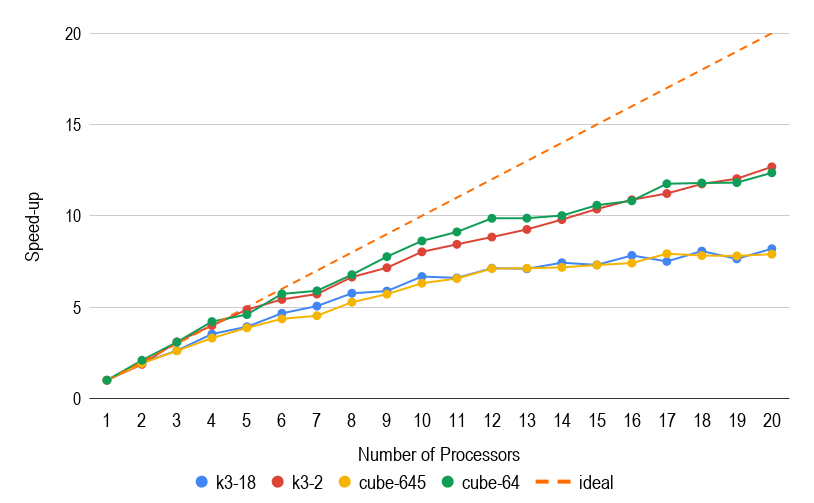
\includegraphics[width=0.8\textwidth]{figures/chapter-2/gmres-strong-scaling-speedup.png}
\caption{GMRES strong scaling speed-up}
\label{fig:gmres-strong-scaling-speed-up}
\end{figure}



% start discussion about preconditioning
The most important criteria of Krylov methods is convergence rate. The convergence rate of iterative methods strongly depends on a matrix and, in particular, on its condition number. For instance, equation \ref{eq:Gmres-7} shows dependence of the convergence rate from the matrix condition number. It can be clearly seen that a big condition number leads to very slow error reduction and, as the results, to huge number of iterations.\\

\begin{equation} \label{eq:Gmres-7}
	|| e^i ||_A \leq 2 ( \frac{\sqrt k - 1}{\sqrt k + 1} )^i || e^0 ||_A
\end{equation}

where $k = \frac{\lambda_{max}}{\lambda_{min}}$ - condition number of the corresponding matrix. \\

An obvious solution of such a problem is to reduce the condition number of the original system \ref{eq:slq}. A general method is to transform the original system in such a way that the conditional number of the transformed system gets significantly smaller. The transformation of \ref{eq:slq} can be done from the left side \ref{eq:pcn-1} or from the right one \ref{eq:pcn-2}.

\begin{equation} \label{eq:pcn-1}
	PAx = Pb
\end{equation}


\begin{equation} \label{eq:pcn-2}
	AP(P^{-1}x) = b
\end{equation}

where matrix $P$ is called preconditioner.\\


As an extreme example we can consider the inverse matrix $A^{-1}$ as the best preconditioner since it directly leads to the solution of the problem \ref{eq:slq} and, thus, it requires only one iteration. However, it is obvious that computation of inverse $A^{-1}$ is extremely expensive operation and it is not an objective of any iterative methods. That example helps understand and set requirements for preconditioners, namely:

\begin{enumerate}
	\item cheap to compute e.g. a 5-10 iterations of the corresponding Krylov solver
	\item should lead to a small conditioner number of the transposed system
	\item should be sparse, otherwise storage requirements will considerably increase
\end{enumerate}


There exist numerous techniques to compute preconditioners given a matrix $A$ e.g. (point) Jacobi, Block-Jacobi, incomplete $LU$ decomposition (ILU), multilevel ILU (ILU(p)), threshold ILU (ILUT), incomplete Cholesky factorization (IC), sparse approximate inverse (SPAI), multigrid as a preconditioner, etc. Almost all methods listed above have some tuning parameters which allow to get a better preconditioner i.e. a smaller condition number of the transformed system. However, it usually leads to increase of computational and storage costs. \\

Some methods can works particularly well for matrices derived from certain PDEs e.g. Poisson, Navier\-Stokes, etc. problems discretized using the cartesian grid. However sometimes it can take a considerable amount of time to choice right parameters for a certain preconditioning algorithm. It can become a challenge to fulfill all requirements 1, 2, 3 mentioned above. \\

Table \todo{Table with comparisons of different preconditioning for our test cases}

Table [] shows results of different preconditioning algorithms application to our test case. It can be seen that some algorithms failed even after tuning. \\

It interesting to notice that \citeauthor{wsmp} came to approximately the same results working on their set of matrices in their work \cite{wsmp}. They observed that preconditioned iterative solvers worked efficiently only for 2 out 5 cases in contrast to direct sparse solvers.\\

We can summarize that it is vital to perform careful parameter tuning of any preconditioning algorithms combining results from [table] and \cite{wsmp}. In general the  search can take a considerable amount of time. Moreover, it becomes impractical for time integration problems where topology of an underlying problem and, as the results, the computational mesh, discretization, Jacobian matrix can be changed over time of a simulation. It is obvious that parameters chosen for a particular time step can become not optimal for consecutive steps and, at the end, it can lead to divergence. If divergence happens at any time step the entire time integration algorithm fails and the simulation has to be restarted with different preconditioning parameters or with a different preconditioning algorithm.\\

By and large we come to a conclusion that preconditioned iterative solvers are not robust and thus cannot fully fulfill requirements listed in section \ref{chapter:solver configuration}.\\

% maybe above we have to mention inderect memory access and its effect on performance


\section{Direct Sparse Methods}
\section{Direct sparse methods}
\label{subseq:sparse methods}

Direct sparse methods combine main advantages of direct and iterative methods i.e. numerical robustness and usage of sparsity structures. As a results, there is no need for preconditioning and the computation complexity is $O(n^2)$ \cite{complexity-of-spdm}. The problem is that storage cost can significantly increase during factorization i.e. the inverse of a sparse matrix can be sufficiently dense. To reduce storage space of $LU$ decomposition this group of methods performs fill-in reduction reodering as a pre-processing step before actual factorization. If storage space is still huge even after fill-in reduction reodering out-of core factorization can be used where partial results are stored in the secondary memory. \\

The most widely known sparse direct method is multifrontal method introduced by \citeauthor{mult-frontal-original:1} in their work \cite{mult-frontal-original:1}. Multifrontal method is an improved extension of a frontal method \cite{frontal-original} that can compute independent fronts in parallel. A front, or also called frontal matrix, can be considered as small dense matrix which is a result of Gaussian Elimination for a particular column. The algorithm, in fact, is as a variant of Gaussian Elimination process. There also exist left-looking and right-looking sparse direct methods. The difference between all of them is explained and can be found in \cite{elimination-tree}.\\


In order to understand and analyze strong scaling behavior of the algorithm we have to briefly discuss the theory of the method. For simplicity we will assume that matrix $A$ is real symmetric and $LU$ decomposition boils down to the Cholesky factorization \ref{eq:chol-1}. It allows us to focus on the Cholesky factor $L$ and its sparsity pattern only.

\begin{equation} \label{eq:chol-1}
	A = LDL^T
\end{equation}

The algorithm usually starts with symbolic factorization to predict sparsity pattern of $L$. Once it is done the corresponding elimination tree has to be constructed.\\

\figpointer{\ref{fig:sparsity-pattern-example-mm}}

\begin{figure}[htpb]
  \centering
  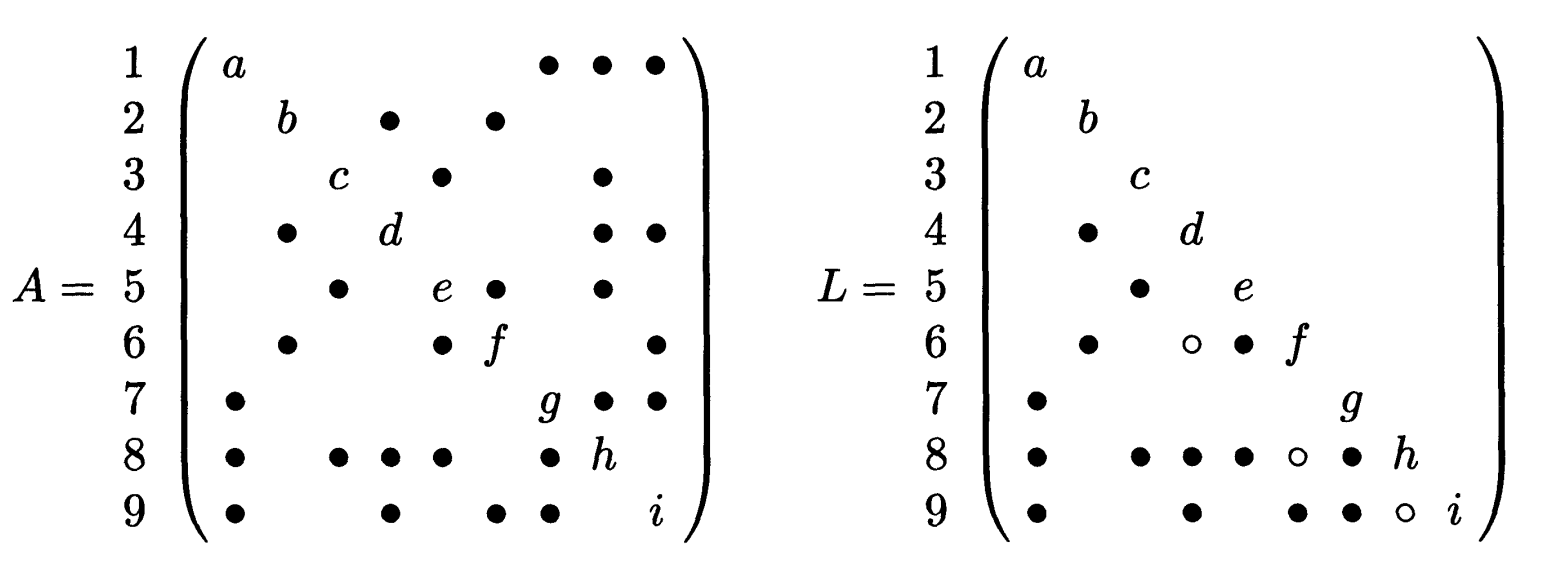
\includegraphics[width=0.9\textwidth]{figures/chapter-2/sparsity-pattern-example-mm.png}
\caption{An example of a sparse matrix and its Cholesky factor \cite{mult-frontal-original:2}}
\label{fig:sparsity-pattern-example-mm}
\end{figure}


Figure \ref{fig:sparsity-pattern-example-mm} shows an illustrative example of a sparse matrix and its Cholesky factor from \cite{mult-frontal-original:2}. The solid circles represent original non-zero elements whereas hollow ones define fill-in factors of $L$. \\


The elimination tree is a crucial part of the method. It can be considered as a structure of $n$ nodes that node $p$ is the parent of $j$ if and only if it satisfies equation \ref{eq:elimination-tree-1}. It is worth pointing out the definition \ref{eq:elimination-tree-1} is not only one possible and one can define a strucutre of an elimination tree in a different way as well. As an example one can find a definition of a general assembly tree in \cite{mult-frontal-original:2} proposed by \citeauthor{mult-frontal-original:2}.\\

\begin{equation} \label{eq:elimination-tree-1}
	p = min(i > j | l_{ij} \neq 0)
\end{equation}


It is important to notice that node $p$ represents elimination process of the corresponding column $p$ of matrix $A$ as well as all dependencies of column $p$ factorization on the results of its descendants.\\


Given definition \ref{eq:elimination-tree-1} we can build the corresponding elimination tree as it is shown in figure \ref{fig:elimination-tree-mm}.\\


\figpointer{\ref{fig:elimination-tree-mm}}

\begin{figure}[htpb]
  \centering
  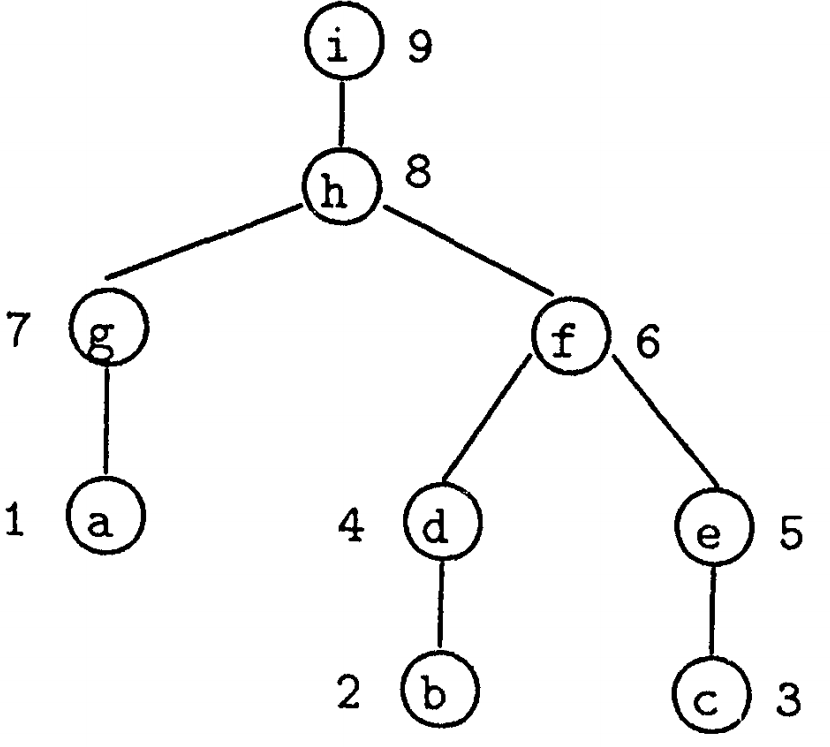
\includegraphics[width=0.45\textwidth]{figures/chapter-2/elimination-tree-mm.png}
\caption{The elimination tree for the matrix example in Figure \ref{fig:sparsity-pattern-example-mm}
 \cite{mult-frontal-original:2}}
\label{fig:elimination-tree-mm}
\end{figure}


The fundamental idea of multifrontal method spins around frontal and update matrices. A frontal matrix is used to perform Gaussian Elimination for a specific column $j$. It is a sum of a frame and update matrices as it can be seen from equation \ref{eq:mm-1}\\.

\begin{equation} \label{eq:mm-1}
	F_{j} = Fr_{j} + \hat{U_{j}} = \begin{bmatrix}a_{j,j} & a_{j,i_1} & a_{j,i_2} & \dots & a_{j,i_r} \\
a_{i_1,j} \\
a_{i_1,j} \\
\vdots & & & 0\\
a_{i_r,j} \\
\end{bmatrix} + \hat{U_{j}}
\end{equation}

where $i_{0}$, $i_{1}$, \dots , $i_{r}$ are the row subscripts of non-zeros in $L_{*j}$ with $i_{0} = j$ and $r$ is number of off-diagonal non-zero elements.\\

The frame matrix $Fr_{j}$ is filed with zeros except the first row and column. The first row and column contain non-zeros elements of the $j$th row and column of the original matrix $A$. Because we consider matrix $A$ to be symmetric the frame matrix is square and symmetric as well.\\

In order to describe parts of the elimination tree we will use the notation $T[j]$ to represent all descendants of the node $j$ in the tree and node $j$ itself. In this way we can define the update matrix $\hat{U_{j}}$ as following:\\

\begin{equation} \label{eq:mm-2}
	\hat{U_{j}} = - \sum_{k \in T[j] -{j}}  \begin{bmatrix}
l_{j,k} \\
l_{i_1,k} \\
\vdots \\
l_{i_1,k} \\
\end{bmatrix} \begin{bmatrix}
l_{j,k} & l_{i_1,k} & \dots & l_{i_1,k}
\end{bmatrix} 
\end{equation}


The update matrix $\hat{U_{j}}$ is, in fact, can be considered as the second term of the Schur complement i.e. update contributions from already factorized columns of $A$.\\

The subscript $k$ represents descendant columns of node $j$. Thus we include and consider only those elements of descendant columns which correspond to the non-zero pattern of the $j$th column that we are currently factorizing.\\

Let's consider the partial factorization of 2-by-2 block dense matrix to better understand essence of update matrix $\hat{U_{j}}$.\\


\begin{equation} \label{eq:mm-3}
A = \begin{bmatrix}
B & V^{T} \\
V & C
\end{bmatrix} 
= 
\begin{bmatrix}
L_{B} & 0 \\
VL^{-T}_{B} & I
\end{bmatrix}
\begin{bmatrix}
I & 0 \\
0 & C - VB^{-1}V^{T}
\end{bmatrix} 
\begin{bmatrix}
L^{T}_{B} & L^{-1}_{B}V^{T} \\
0 & I
\end{bmatrix} 
\end{equation}

Again we assume that $B$ has already been factorized and can be expressed as:

\begin{equation} \label{eq:mm-4}
	B = L_{B}L^{T}_{B}
\end{equation}

The Schur complement from equation \ref{eq:mm-3} can be viewed as the original sub-matrix $C$ and update $-VB^{-1}V^{T}$. It can be written in a vector form as well:

\begin{equation} \label{eq:mm-5}
	-VB^{-1}V^{T} = -(VL^{-T}_{B})(L^{-1}_{B}V^{T}) = - \sum_{k=1}^{j-1}  \begin{bmatrix}
l_{j,k} \\
\vdots \\
l_{n,k} \\
\end{bmatrix} \begin{bmatrix}
l_{j,k} & \dots & l_{n,k}
\end{bmatrix} 
\end{equation}

As it can be easily seen that equations \ref{eq:mm-5} and \ref{eq:mm-2} are identical. The difference is that equation \ref{eq:mm-2} exploits sparsity of the corresponding row and column of $L$ and thus masks unnecessary information. \\

% both eqautions show that the update matrix aggregate all previous information done and in case of the ,ultifrontal methods it means that we aggregate all information from descendants

% Therefore, we can express Uy as an aggregate of outer- product updates from columns in T[Cl],..., T[cs]. 

We can also notice from equation \ref{eq:mm-3} that the frame matrix $Fr_{j}$ corresponds to the block matrix $C$ and brings information from the original matrix $A$ whereas matrix $\hat{U_{j}}$ adds information about the columns that have already been factorized.\\

As soon as the frontal matrix $F_{j}$ is assembled i.e. we have the complete update of column $j$, we can perform elimination of the first column and get non-zero entries of factor column $L_{*j}$.\\

Let's denote $\hat{F_{j}}$ as a result of the first column factorization of the frontal matrix $F_{j}$. Then we can express the results as following:\\


\begin{equation} \label{eq:mm-6}
\hat{F_{j}} = \begin{bmatrix}
l_{j,j} & \dots & 0 \\
\vdots & I \\
l_{i_{r},j} \\
\end{bmatrix} 
\begin{bmatrix}
1 & \dots & 0 \\
\vdots & U_{j} \\
0 \\
\end{bmatrix} 
\begin{bmatrix}
l_{j,j} & \dots & l_{i_{r},j} \\
\vdots & I \\
0 \\
\end{bmatrix} 
\end{equation}

where sub-matrix $U_{j}$ represents the full update from all descendants of node $j$ and node $j$ itself. Equation \ref{eq:mm-7} express the sub-matrix $U_{j}$ in a vector form.\\

\begin{equation} \label{eq:mm-7}
\hat{U_{j}} = - \sum_{k \in T[j]}  \begin{bmatrix}
l_{i_1,k} \\
\vdots \\
l_{i_1,k} \\
\end{bmatrix} \begin{bmatrix}
l_{i_1,k} & \dots & l_{i_1,k}
\end{bmatrix}
\end{equation}

Together with the frontal $F_{j}$ and update $\hat{U_j}$ matrices, the update column matrix $U_{j}$ (also called contribution matrices) forms the key concepts of the multifrontal method. To consider the importance of sub-matrix $U_{j}$ let's consider and example illustrated in Figure \ref{fig:information-float}.\\

\figpointer{\ref{fig:information-float}}
\begin{figure}[htpb]
  \centering
  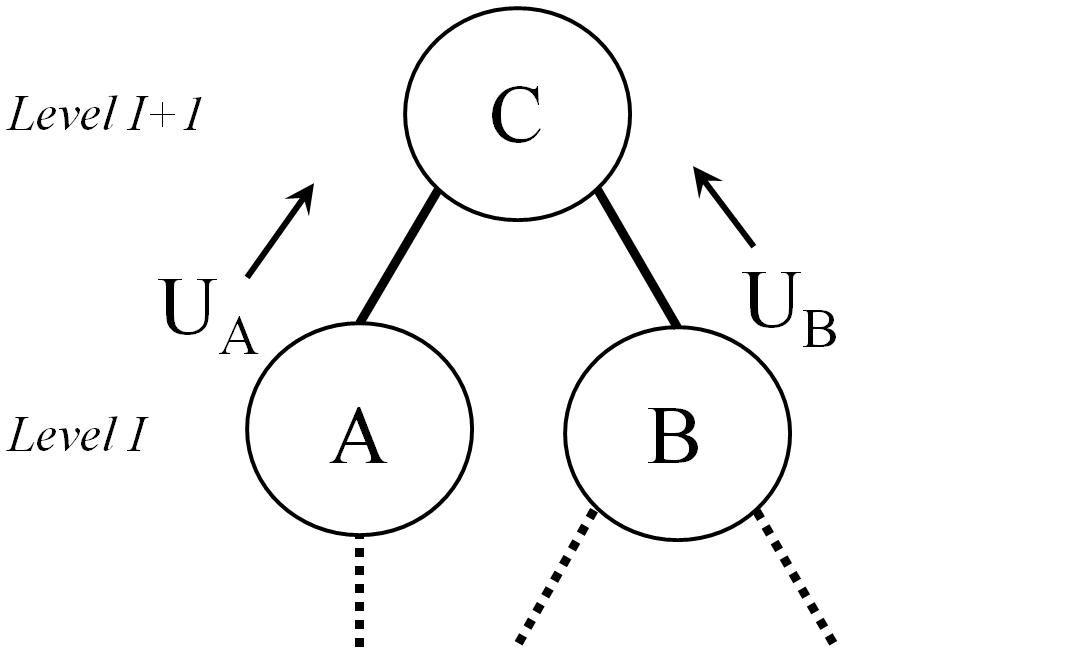
\includegraphics[width=0.45\textwidth]{figures/chapter-2/information-flow.png}
\caption{Information flow of the multifrontal method}
\label{fig:information-float}
\end{figure}


We assume that factorization of columns A and B have already been done and corresponding contribution matrices $U_{A}$ and $U_{B}$ have been computed. From equation \ref{eq:mm-7} we have already known that both $U_{A}$ and $U_{B}$ contain the full updates of all their descendants including updates from factorization of columns $A$ and $B$ as well. Therefore update column matrices $U_{A}$ and $U_{B}$ have already got all necessary information to construct update matrix $\hat{U_{C}}$. The detailed proof and careful explanation can be found in \cite{mult-frontal-original:2}.\\


It might happen that we do not need all rows and columns of $U_{A}$ and $U_{B}$ i.e. we need only some subset of them, because of sparsity of column $C$ . It is also important to place all necessary rows and columns of matrices $U_{A}$ and $U_{B}$ in a right place within matrix $\hat{U_{C}}$. For that reason, an additional matrix operation, called \textbf{\textit{extend-add}}, must be introduced.\\

Let's consider an example from \cite{mult-frontal-original:2} of an extend-add operation for 2-by-2 matrices $R$ and $S$ which correspond to the indices ${5,8}$ and ${5,9}$ of some matrix $B$, respectively.\\

\begin{equation}
R = \begin{bmatrix}
p & q \\
u & v \\
\end{bmatrix} 
,
\:
S = \begin{bmatrix}
w & x \\
y & z \\
\end{bmatrix} 
\end{equation}

The result of the operation is going to be a 3-by-3 $K$ matrix which looks as following:\\

\begin{equation} \label{eq:mm-8}
K = R \extendadd S = \begin{bmatrix}
p & q & 0 \\
u & v & 0 \\
0 & 0 & 0 \\
\end{bmatrix} 
+
\begin{bmatrix}
w & 0 & x \\
0 & 0 & 0 \\
y & 0 & z \\
\end{bmatrix} 
=
\begin{bmatrix}
p + w & q & x \\
u & v & 0 \\
y & 0 & z \\
\end{bmatrix} 
\end{equation}

Hence we can express formation of the frontal matrix $F_{j}$ using the extend-add operation and all direct children of node $j$ in the following way:


\begin{equation} \label{eq:mm-9}
	F_{j} = \begin{bmatrix}a_{j,j} & a_{j,i_1} & a_{j,i_2} & \dots & a_{j,i_r} \\
a_{i_1,j} \\
a_{i_1,j} \\
\vdots & & & 0\\
a_{i_r,j} \\
\end{bmatrix} \extendadd U_{c_1} \extendadd \dots \extendadd U_{c_s} 
\end{equation}

where $c_{1}, \: c_{2}, \: \dots \: c_{n}$ are indices of direct children of the node $j$.\\

Now it can be clearly seen that the resultant frontal matrix $F_{j}$ is a small dense one and it can be efficiently computed using BLAS level 3 subroutines.\\

After factorization we have to build the contribution matrix $U_{j}$ i.e. add columns and rows of $U_{c_1}, \:, U_{c_2}, \: \dots, U_{c_s}$ to $U_{j}$ that have not been used in factorization of $F_{j}$ due to sparsity of column $j$. After that we can continue to move up along the tree. 
The complete update matrices grow in size as we move to the top of the tree. Therefore they have to be stored in a sparse matrix format to stay within memory constrains of the computer.\\


Another important aspect is storage and manipulation of frontal and contribution matrices. Sometimes we have to store contribution matrices produced in previous steps into some temporary buffer and efficiently retrieve them later during factorization. This can require some matrix re-ordering. In case of symmetric matrices, one can apply postordering on a tree to be able to use the stack data structure to alleviate the process of contribution matrix manipulations during factorization. A tree postordering is based on topological ordering and it has been proven that it is equivalent to the original matrix ordering and thus leads to the same filled graph \cite{mult-frontal-original:2}. \todo{sentence refactoring} We refer to the original matrix ordering as the ordering received from fill-in reduction operation.\\


A tree postordering means that a node is ordered before its parent and, additionally, nodes in each subtree are numbered consecutively. Figure \ref{fig:mm-matrix-postordering} shows an example of posrordering applied to the elimination tree of the matrix from figure \ref{fig:sparsity-pattern-example-mm}. The results of this can be see in figure \ref{fig:mm-contrib-matrix-manipulation} where consecutive \textit{push} and \textit{pop} operations are efficiently used during factorization and thus simplify the program logic.\\


\figpointer{\ref{fig:mm-matrix-postordering}}
\begin{figure}[htpb]
  \centering
  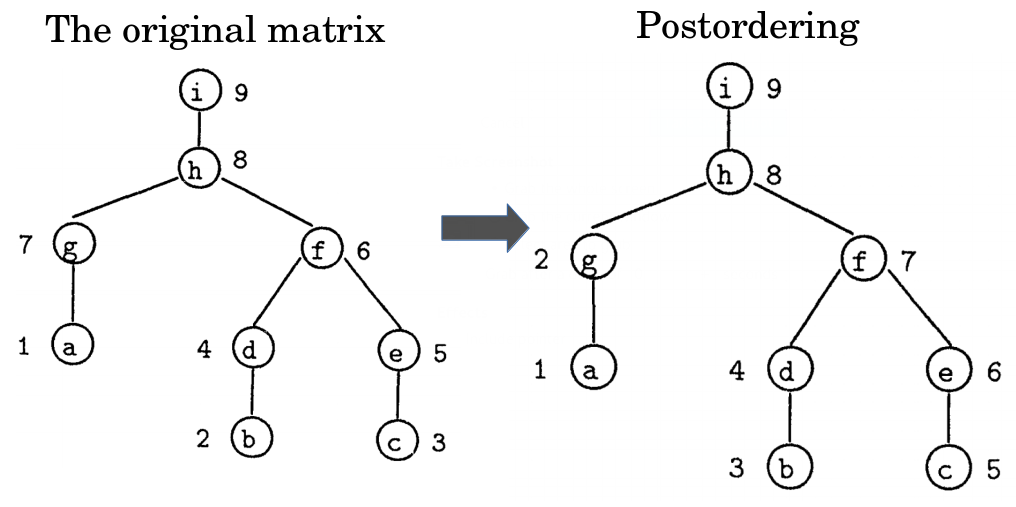
\includegraphics[width=0.75\textwidth]{figures/chapter-2/elimination-tree-mm-postordering.png}
\caption{An example of matrix postordering from \cite{mult-frontal-original:2}}
\label{fig:mm-matrix-postordering}
\end{figure}


\figpointer{\ref{fig:mm-contrib-matrix-manipulation}}
\begin{figure}[htpb]
  \centering
  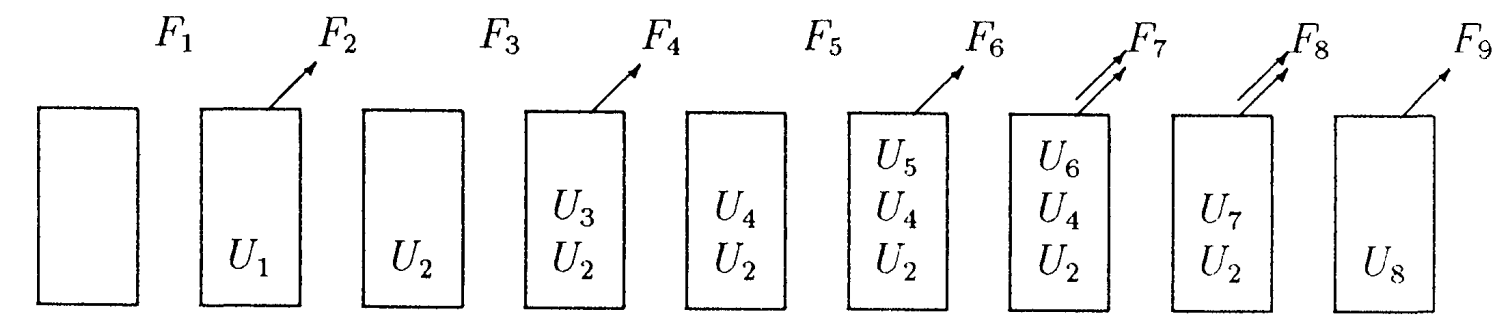
\includegraphics[width=0.75\textwidth]{figures/chapter-2/mm-contrib-matrix-manipulation.png}
\caption{The stack contents for the postordering \cite{mult-frontal-original:2}}
\label{fig:mm-contrib-matrix-manipulation}
\end{figure}


We can see the algorithm requires to perform some preprocessing steps in order to estimate the size of working space for matrix manipulations. If the working space has not been predicted correctly the algorithm will terminate during factorization. Additionally it can happen that even with the correct estimation we can be run out of space in the main memory, in case of huge sparse matrices. This fact can require to use the secondary memory and, as a result, the execution time will increase significantly. Therefore, different optimal postordering schemes have been proposed which allow to shrink the amount of space needed during factorization \cite{mm:optimal-tree-postordering} \cite{mm:elimination-tree-rotations}. Some schemes, for example elimination tree rotations \cite{mm:elimination-tree-rotations}, can lead to deep and unbalanced trees which might have their negative effect on task parallelism as we will see later.\\


In general, the estimation of working space can be tricky due to pivoting. Because pivoting happens only during the numerical factorization it is not always possible to estimate enough space correctly beforehand. There exist some heuristics which allow to use some numerical matrix information during symbolic factorization to better predict the amount of required space \cite{wsmp:direct-solution-of-general-system}.\\



It can be clearly observed the method consists of three distinct phases, namely: analysis, numerical factorization and solution. The analysis phase includes all pre-processing steps that have been discussed above i.e. fill-in reduction, postordering, symbolic factorization, building elimination tree an so on. During the numerical factorization phase the $L$ and $D$ (or $U$) parts of a matrix $A$ are computed based on sequence of dense factorization on frontal matrices. At the solution step, the solution vector $x$ is computed by means of backward and forward substitutions (equations \ref{eq:lu} and \ref{eq:bk}).\\


% supernodal
In practice, an improved version of multifrontal method, called supernodal method, is used. The idea of the supernodal method is to shrink the final elimination tree by grouping some particular nodes/columns in one computational unit. As a result, more useful floating point operations per memory access can be performed by eliminating few columns at once within the same frontal matrix.\\


% FOR PRESENTATION: Working on supernodes instead of individual variables is essential in order to speed-up the computations and use high-level BLAS [72] (Basic Linear Algebra Subprograms): supernodes lead to a higher flops to memory access ratio, and this allows a better usage of memory hierarchy and better performance thanks to the blocking techniques used in BLAS routines.



A supernode is formed by a set of contiguous columns with identical off-diagonal sparsity structure forms. Thus, a supernode has few important properties. Firstly, it can be expressed as a set of indices, namely: $\{j, \: j+1, \: \dots, \:j + t\}$, where node $j + k$ is	parent of $j + k - 1$ in the elimination tree. Secondly, the size of the supernodal frontal matrix is equal to the frontal matrix of the $j$th column within a supernode. As an example, Figure \ref{fig:supernodal-method-postordering-and-etree} shows a postordered matrix $A$ and its Cholesky factor $L$ as well as the corresponding supernodal elimination tree.


\figpointer{\ref{fig:supernodal-method-postordering-and-etree}}

\begin{figure}[htpb]
  \centering
  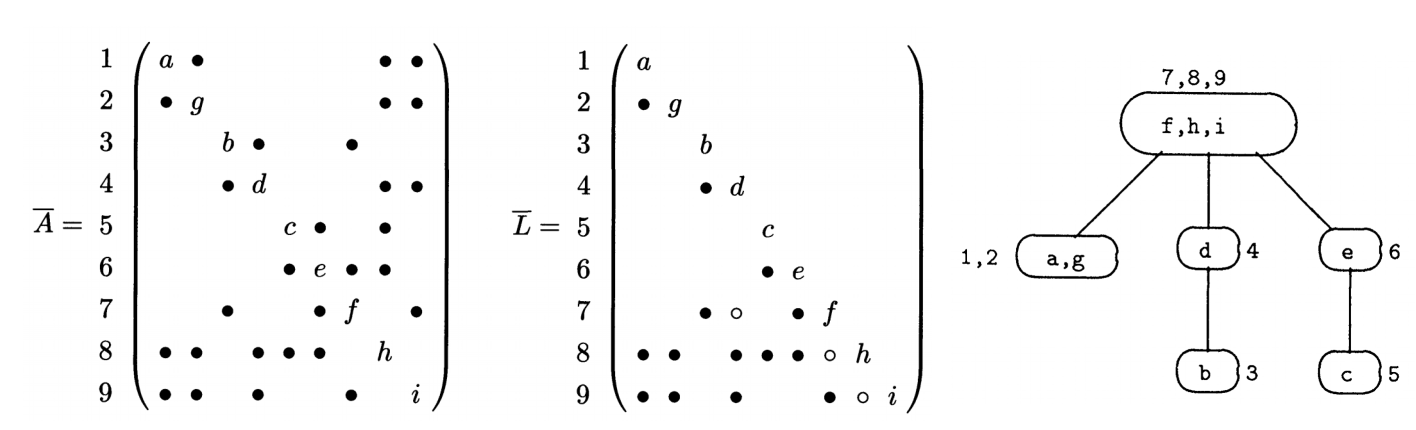
\includegraphics[width=1.0\textwidth]{figures/chapter-2/supernodal-method-postordering-and-etree.png}
\caption{An example of a supernodal elimination tree \cite{mult-frontal-original:2}}
\label{fig:supernodal-method-postordering-and-etree}
\end{figure}
 
 
Equation \ref{eq:mm-10} expresses the building process of a frontal matrix of a supernode. In contrast to \ref{eq:mm-9}, the frame matrix $\mathcal{F}_{j}$ contains more dense rows and columns. As before, we use \textit{extend-add} operation to get the full block update from children contribution matrices.\\


\todo{check grammar}
It should be mentioned there exist more sophisticated variants of supernodes. Most of the time, it intends to improve efficiency of the algorithm. \citeauthor{mult-frontal-original:2} pointed out that supernodes could be defined without using the contiguous constrains \cite{mult-frontal-original:2}. On another hand, \citeauthor{complexity-of-spdm} defines supernodes corresponded to separators from the nested dissection step  \cite{complexity-of-spdm} which was used for fill-in reduction.\\



 \begin{equation} \label{eq:mm-10}
	\mathcal{F}_{j} = \begin{bmatrix}a_{j,j} & a_{j,j+1} & \dots & a_{j,j+t}  & a_{j,i_1} & \dots & a_{j,i_r} \\
a_{j+1,j} & a_{j+1,j+1} & \dots & a_{j+1,j+t}  & a_{j+1,i_1} & \dots & a_{j+1,i_r} \\
\vdots & \vdots & \dots & \vdots \\
a_{j+t,j}  & a_{j+t,j+1} & \dots & a_{j+t,j+t}  & a_{j+t,i_1} & \dots & a_{j+t,i_r} \\
a_{i_1,j} & a_{i_1,j+1} & \dots & a_{i_1,j+t} \\
\vdots & \vdots & \dots & \vdots  & & 0\\ 
a_{i_r,j} & a_{i_r,j+1} & \dots & a_{i_r,j+t} \\
\end{bmatrix} \extendadd U_{c_1} \extendadd \dots \extendadd U_{c_s} 
\end{equation}


Up to this point we have already seen all key concepts of the multifrontal method and discussed how the algorithm works. We will move to the discussion of parallelization of the method. \\


The elimination tree, in fact, represents dependencies among columns. Conversely, the tree also shows independent steps of elimination process. Hence the tree forms independent problems that can be executed in parallel. Task parallelism is the main and primary source the algorithm parallelisation. Figure \ref{fig:elimination-tree-mm-parallel-steps} shows task parallelism, for the example given in Figure \ref{fig:supernodal-method-postordering-and-etree}, where each color represents a set concurrent tasks.\\


\figpointer{\ref{fig:elimination-tree-mm-parallel-steps}}

\begin{figure}[htpb]
  \centering
  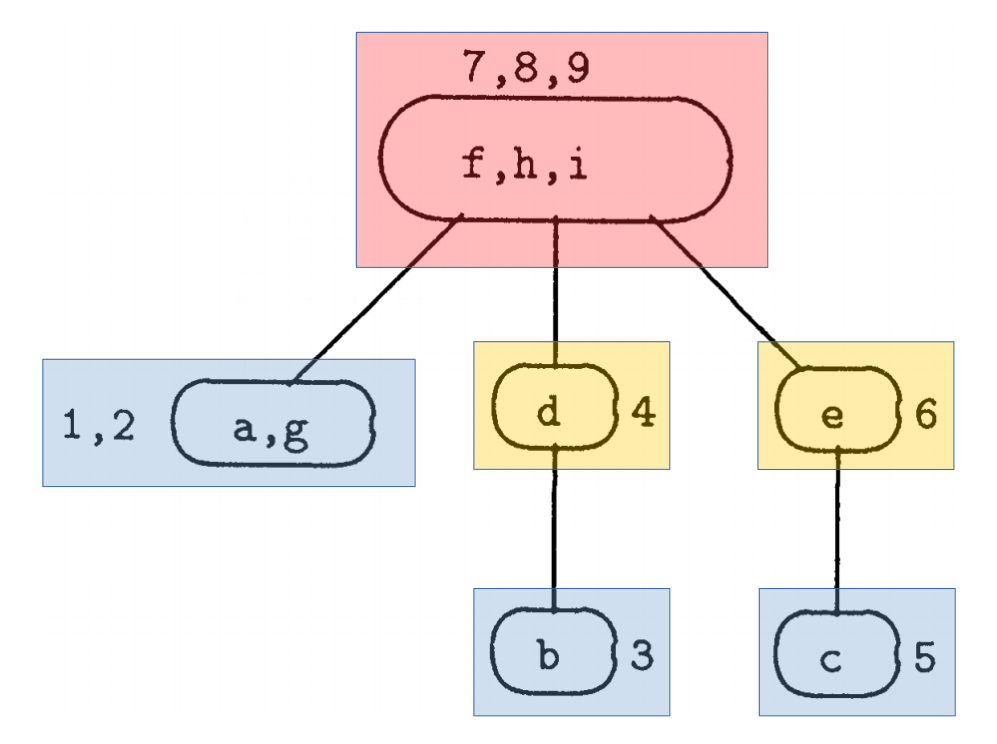
\includegraphics[width=0.5\textwidth]{figures/chapter-2/elimination-tree-parallel.png}
\caption{Parallel steps of the multifrontal method based on the example in Figures \ref{fig:supernodal-method-postordering-and-etree}}
\label{fig:elimination-tree-mm-parallel-steps}
\end{figure}


For example, nodes on separate branches of the tree are totally independent and can processed in parallel. However, as soon as at least two branches run into the same node it forms a dependency and we have to wait all contribution matrices of its children and cannot proceed further.\\ 


We can observe the amount of task parallelism is rapidly decreasing while moving towards the root along the tree. Once we reach the root of the tree the algorithm becomes totally sequential. This fact can play the significant role in strong scaling behavior of the method.\\


We developed two simple models based on perfectly balanced binary trees to better understand strong scaling of the algorithm. The main concept of the models is so-called cost per level or cost per node. This idea is similar to the recursion trees in \cite{recursion-tree} which explains and computes complexity of recurrent algorithms.\\


Figure \ref{fig:mm-parallel-model-tree-linear} represents the first model where we keep the same cost per level whereas the second model (Figure \ref{fig:mm-parallel-model-tree-quadratic}) simulates quadratic cost decay from level to level. Additionally we assume that computational cost distributed uniformly between nodes at the same level for both models.\\


\figpointer{\ref{fig:mm-parallel-model-tree}}
\begin{figure}
\centering
	\begin{tabular}{cc}
			\subfloat[Model 1: equal cost per level]{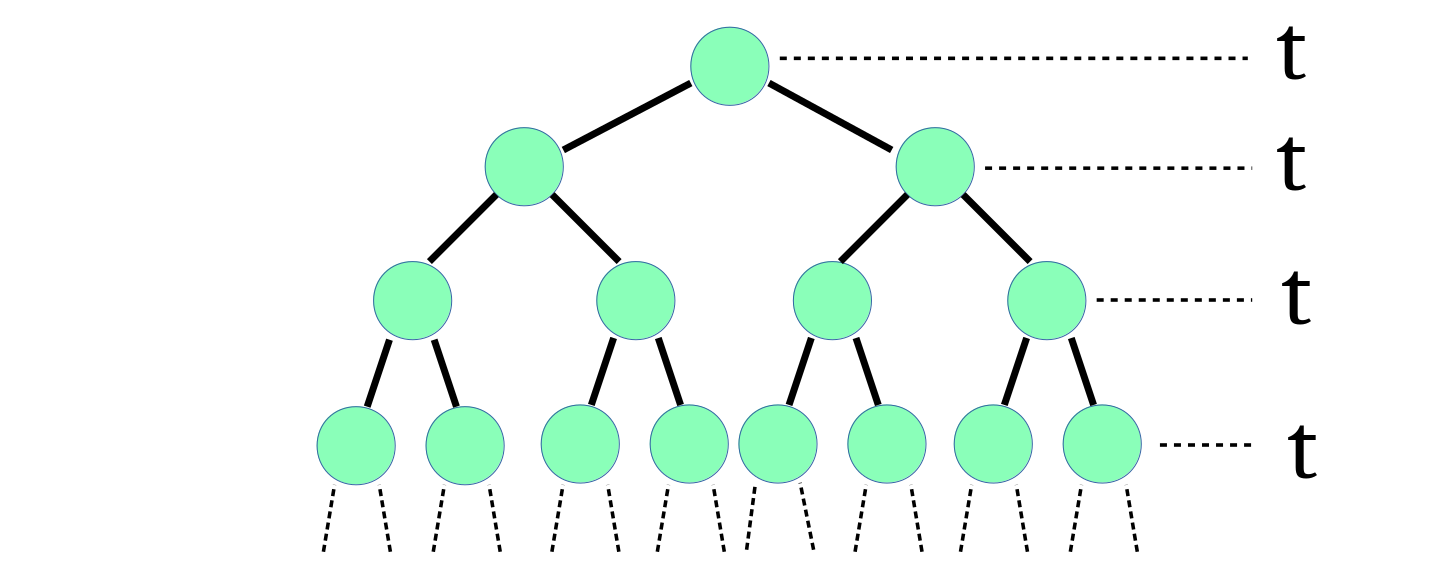
\includegraphics[width=0.5\textwidth]{figures/chapter-2/mm-parallel-model-tree-1.png} \label{fig:mm-parallel-model-tree-linear}} & 
		\subfloat[Model 2: quadratically decreasing cost per level]{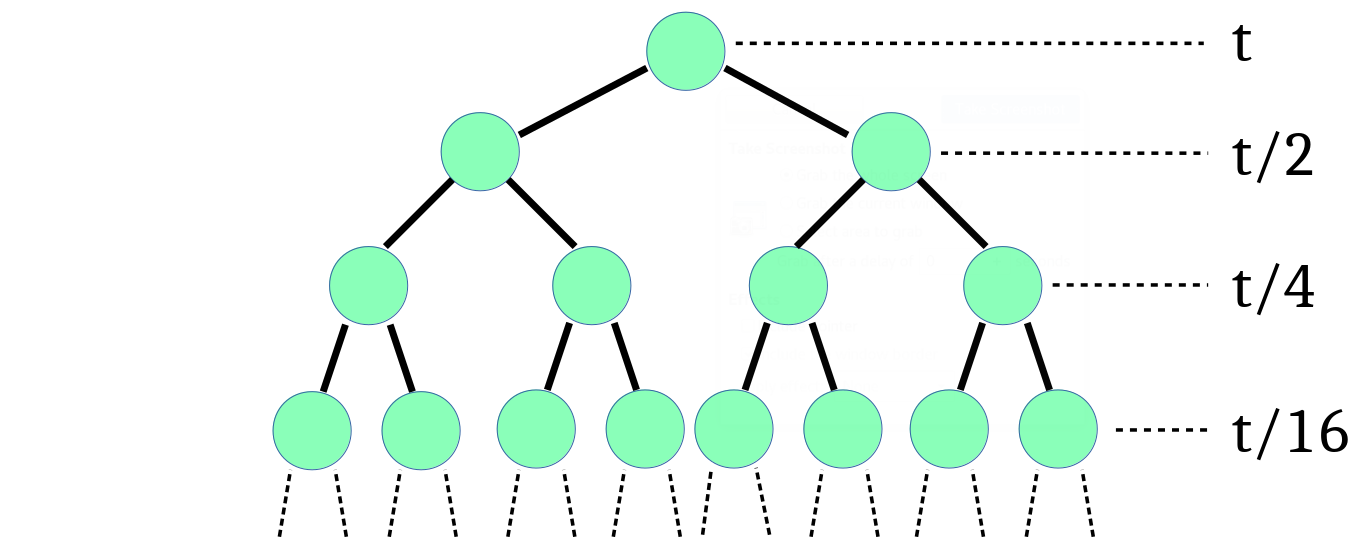
\includegraphics[width=0.5\textwidth]{figures/chapter-2/mm-parallel-model-tree-2.png} \label{fig:mm-parallel-model-tree-quadratic}} \\
	\end{tabular}
	\caption{Simple parallel models of the multifrontal method}
	\label{fig:mm-parallel-model-tree}
\end{figure}

\todo{sentence refactoring}
We have to say that our models mimic only numerical factorization and do not include time spent on any per-processing steps, for example, fill-in reduction reodering. A cost per level can be interpreted in different ways e.g. increase of partial factorization time due to growth of frontal matrices in size, time increase spent on numerical pivoting, increase of MPI communication overheads due to growth of contribution matrices, etc. It should be mentioned that real computer implementations of the multifrontal algorithm (MUMPS, SuperLU, etc.) are quite sophisticated in many aspects and our models do not have any intention to analyze performance of a particular package. Instead the objective of these models is to show possible strong scaling behavior and possible bottlenecks. \\


We will consider only task parallelism at the beginning to a first approximation and later we will discuss how additional data parallelism can affect algorithm performance.\\

% assumtion that cost is equal within the level!!!

Instead of coloring given in Figure \ref{fig:elimination-tree-mm-parallel-steps}, we assume that each level has the same color and thus can be executed fully in parallel if we have enough processing elements. We cannot go to the next level till the current one has not been completed yet i.e. free processing elements, that do not have nodes to execute at the current level, have to wait.\\


As we mentioned above the root of the tree can be processed purely sequentially if we only consider task parallelism. As a first approximation, time spent on the root factorization determines the minimal execution time according to the Amdahl's low \cite{wiki:amdahls-low}. More precisely, the minimal execution time is equal to a sum of time spent on single node partial factorization at each level. This time determines the asymptote on the corresponding speed-up graph.\\


We considered a perfectly balanced tree with 16 levels, 65535 nodes and the maximum of 20 processing elements as an example. The numerical results of linear and quadratic models can be viewed in Figures \ref{fig:mm-parallel-model-tree-linear} and \ref{fig:mm-parallel-model-tree-quadratic}, respectively. The figures show a rapid drop of performance, especially in case of the quadratic model. Table \ref{table:mm-potential-model-speed-up} demonstrates the maximum potential speed-up, having 32768 processing elements which is equal to the number of leaves of the tree, against the speed-up we have got using only 20 processing elements.\\


\figpointer{\ref{fig:mm-parallel-model-speed-up}}
\begin{figure}
\centering
	\begin{tabular}{cc}
			\subfloat[Theoretical speed-up of Model 1]{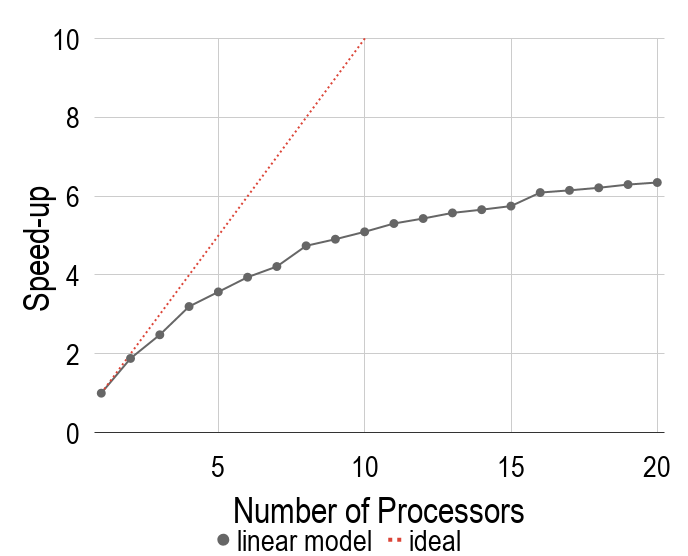
\includegraphics[width=0.45\textwidth]{figures/chapter-2/mm-parallel-model-tree-1-speedup.png}} &
		\subfloat[Theoretical speed-up of Model 2]{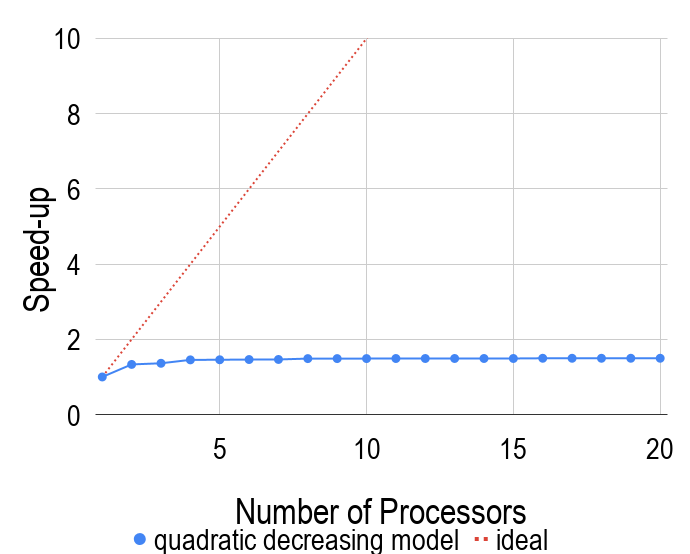
\includegraphics[width=0.45\textwidth]{figures/chapter-2/mm-parallel-model-tree-2-speedup.png}} \\
	\end{tabular}
	\caption{Theoretical speed-up}
	\label{fig:mm-parallel-model-speed-up}
\end{figure}


\begin{table}[htpb]
\centering
\begin{tabular}{|c|c|c|}
\hline
        & 20 PEs  & 32768 PEs \\ \hline
Model 1 & 6.3492  & 8.0000    \\ \hline
Model 2 & 1.4972 & 1.5000   \\ \hline
\end{tabular}
\caption{Potential speed-up of linear and quadratic models}
\label{table:mm-potential-model-speed-up}
\end{table}


We can see that model 1 still has some potential to grow whereas the second model has already reached its asymptote and further increase of processing elements does not make sense. In spite of a potential growth of the first model, both models have very low parallel efficiency even with 20 processing elements which can be observed from table \ref{table:mm-model-efficiency-20-pe}.\\


\begin{table}[htpb]
\centering
\begin{tabular}{|c|c|}
\hline
        & 20 PEs \\ \hline
Model 1 & 0.3175 \\ \hline
Model 2 & 0.0749 \\ \hline
\end{tabular}
\caption{Efficiency of linear and quadratic models using 20 PEs}
\label{table:mm-model-efficiency-20-pe}
\end{table}


Both models shows that computational intensity per node grows from bottom to top. It is easy to conclude from Figure \ref{fig:mm-parallel-model-tree} that intensity per node is equal $t/2^{i}$ and $t/2^{2i}$ for the first and second models, respectively (where $i$ is a level of the tree). It reflects that the most intensive part of the method is centered on the top part of the tree i.e. first few level. \citeauthor{mult-frontal-original:2} discussed application of the multifrontal method to a $k-by-k$ regular model problem with nine-point difference operator in his paper \cite{mult-frontal-original:2}. He observed that factorization of the last 6 nodes took slightly more than 25\% of the total amount of arithmetical operations. As a comparison, table \ref{table:mm-simple-model-work-load} shows fractions of time spent on processing first few top levels of our models: 1 and 2.\\


\begin{table}[htpb]
\centering
\begin{tabular}{|c|c|c|}
\hline
        & Model 1 & Model 2 \\ \hline
Level 0 & 6.25\%  & 50.00\% \\ \hline
Level 1 & 12.50\% & 75.00\% \\ \hline
Level 2 & 18.75\% & 87.50\% \\ \hline

\end{tabular}
\caption{Distribution workload per level in case model 1 and 2}
\label{table:mm-simple-model-work-load}
\end{table}


As we can see, the result of our first model is relatively close to 25\% and, therefore, it looks quite optimistic. However, the second model shows that 87\% of workload is focused on the top part of the tree and, as a result, we can consider that model as extremely pessimistic. \\


By and large, reduction of time spent on the top nodes is a way to improve strong scaling behavior. To do so, data parallelism can be additionally exploited for these nodes. It is worth noting that data parallelism at bottom levels does not make sense because it leads to increase of granularity there and thus increase communication overheads which can lead to significant performance drop.\\


Figure \ref{fig:mumps-task-data-parallelism} shows an example of two types of parallelism applied to the algorithm. First of all, we can see the leaves are grouped in subtrees and a single PE is assigned to each subtree. Other nodes are distributed among three different types. Nodes of the first type uses task parallelism only, which is induced by the tree, and each node is executed in a single processor. The second type exploits data parallelism with 1D block row distribution among the processors. The root belongs to the third type where data parallelism is used with 2D block cyclic distribution. The details of MUMPS parallelism management is carefully explained and can be found in \cite{mumps:task-data-parallelism}.\\


\figpointer{\ref{fig:mumps-task-data-parallelism}}

\begin{figure}[htpb]
  \centering
  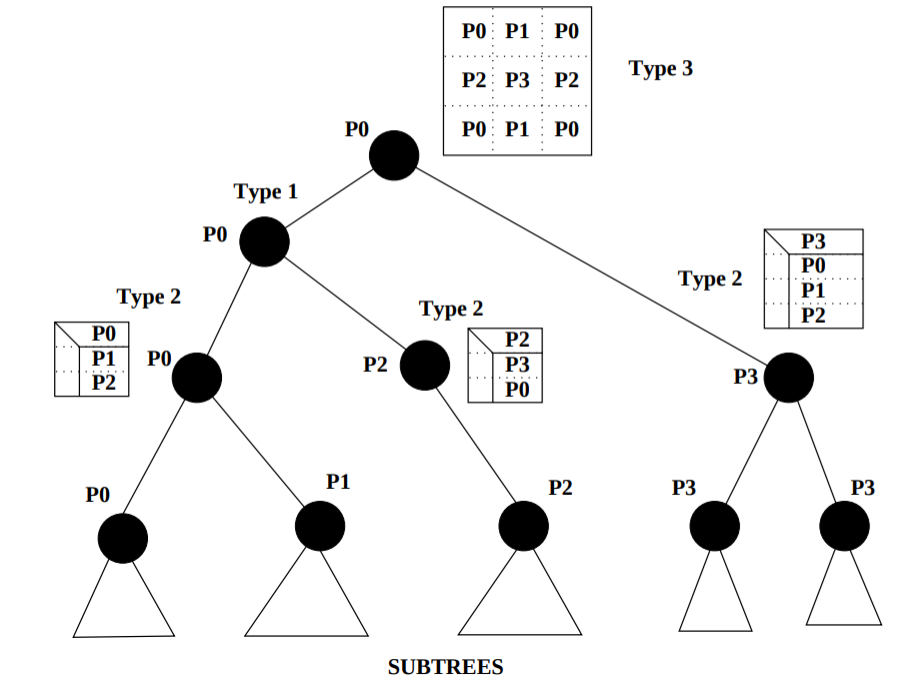
\includegraphics[width=0.65\textwidth]{figures/chapter-2/mumps-task-data-parallelism.png}
\caption{MUMPS parallelism management in case of 4 PEs \cite{mumps:task-data-parallelism}}
\label{fig:mumps-task-data-parallelism}
\end{figure}


All the techniques mentioned above were designed to improve strong scaling behavior by splitting the most intensive parts among all available processors. Going back to our models, we can also think about that in a slightly different way, namely: \textit{data parallelism helps to re-distribute cost per node/level on the corresponding elimination tree}. However, we have to notice that efficiency of data parallelism totally depends on sizes of frontal matrices at the top part of the tree. In case of skinny sparse matrices, oversubscription of processing elements can lead to strong performance penalties as we could see from section \ref{subseq:direct methods}. A machine-dependent minimal frontal matrix size was introduced in MUMPS in order to control whether to use ScaLAPACK at the root node or not \cite{mumps-manual}. It can happen that the algorithm uses only task parallelism, due to the threshold, and, as a results, scaling will only depend on the tree structure that can be deep and unbalanced.\\


Figure \ref{fig:model-1-vs-mumps} shows comparison of strong scaling between model 1 and parallel numerical factorization of the matrix \textit{\textbf{memchip}} (Table \ref{table:suite-sparse-matrix-set}) done with using MUMPS library. The sparsity pattern before and after fill-in reduction is shown in figure \ref{fig:memchip-matrix-sparsity-pattern}. 

\todo{add some examples to the appendix}
\figpointer{\ref{fig:model-1-vs-mumps}. Show standard deviation}
\begin{figure}[htpb]
  \centering
  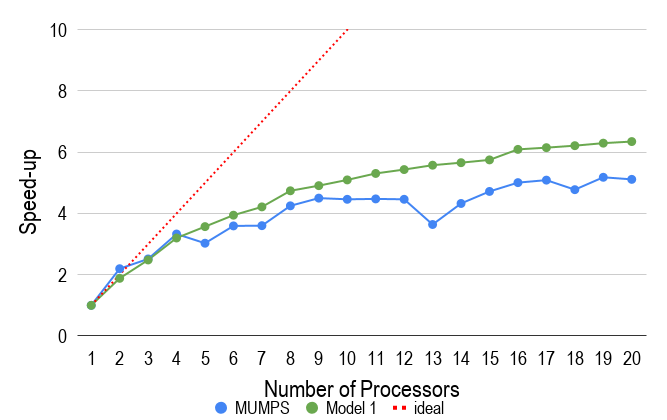
\includegraphics[width=0.65\textwidth]{figures/chapter-2/model-1-vs-mumps.png}
\caption{Comparison between model 1 and numerical factorization of the matrix \textit{\textbf{memchip}} using MUMPS library}
\label{fig:model-1-vs-mumps}
\end{figure}


\figpointer{\ref{fig:memchip-matrix-sparsity-pattern}}
\begin{figure}[htpb]
  \centering
  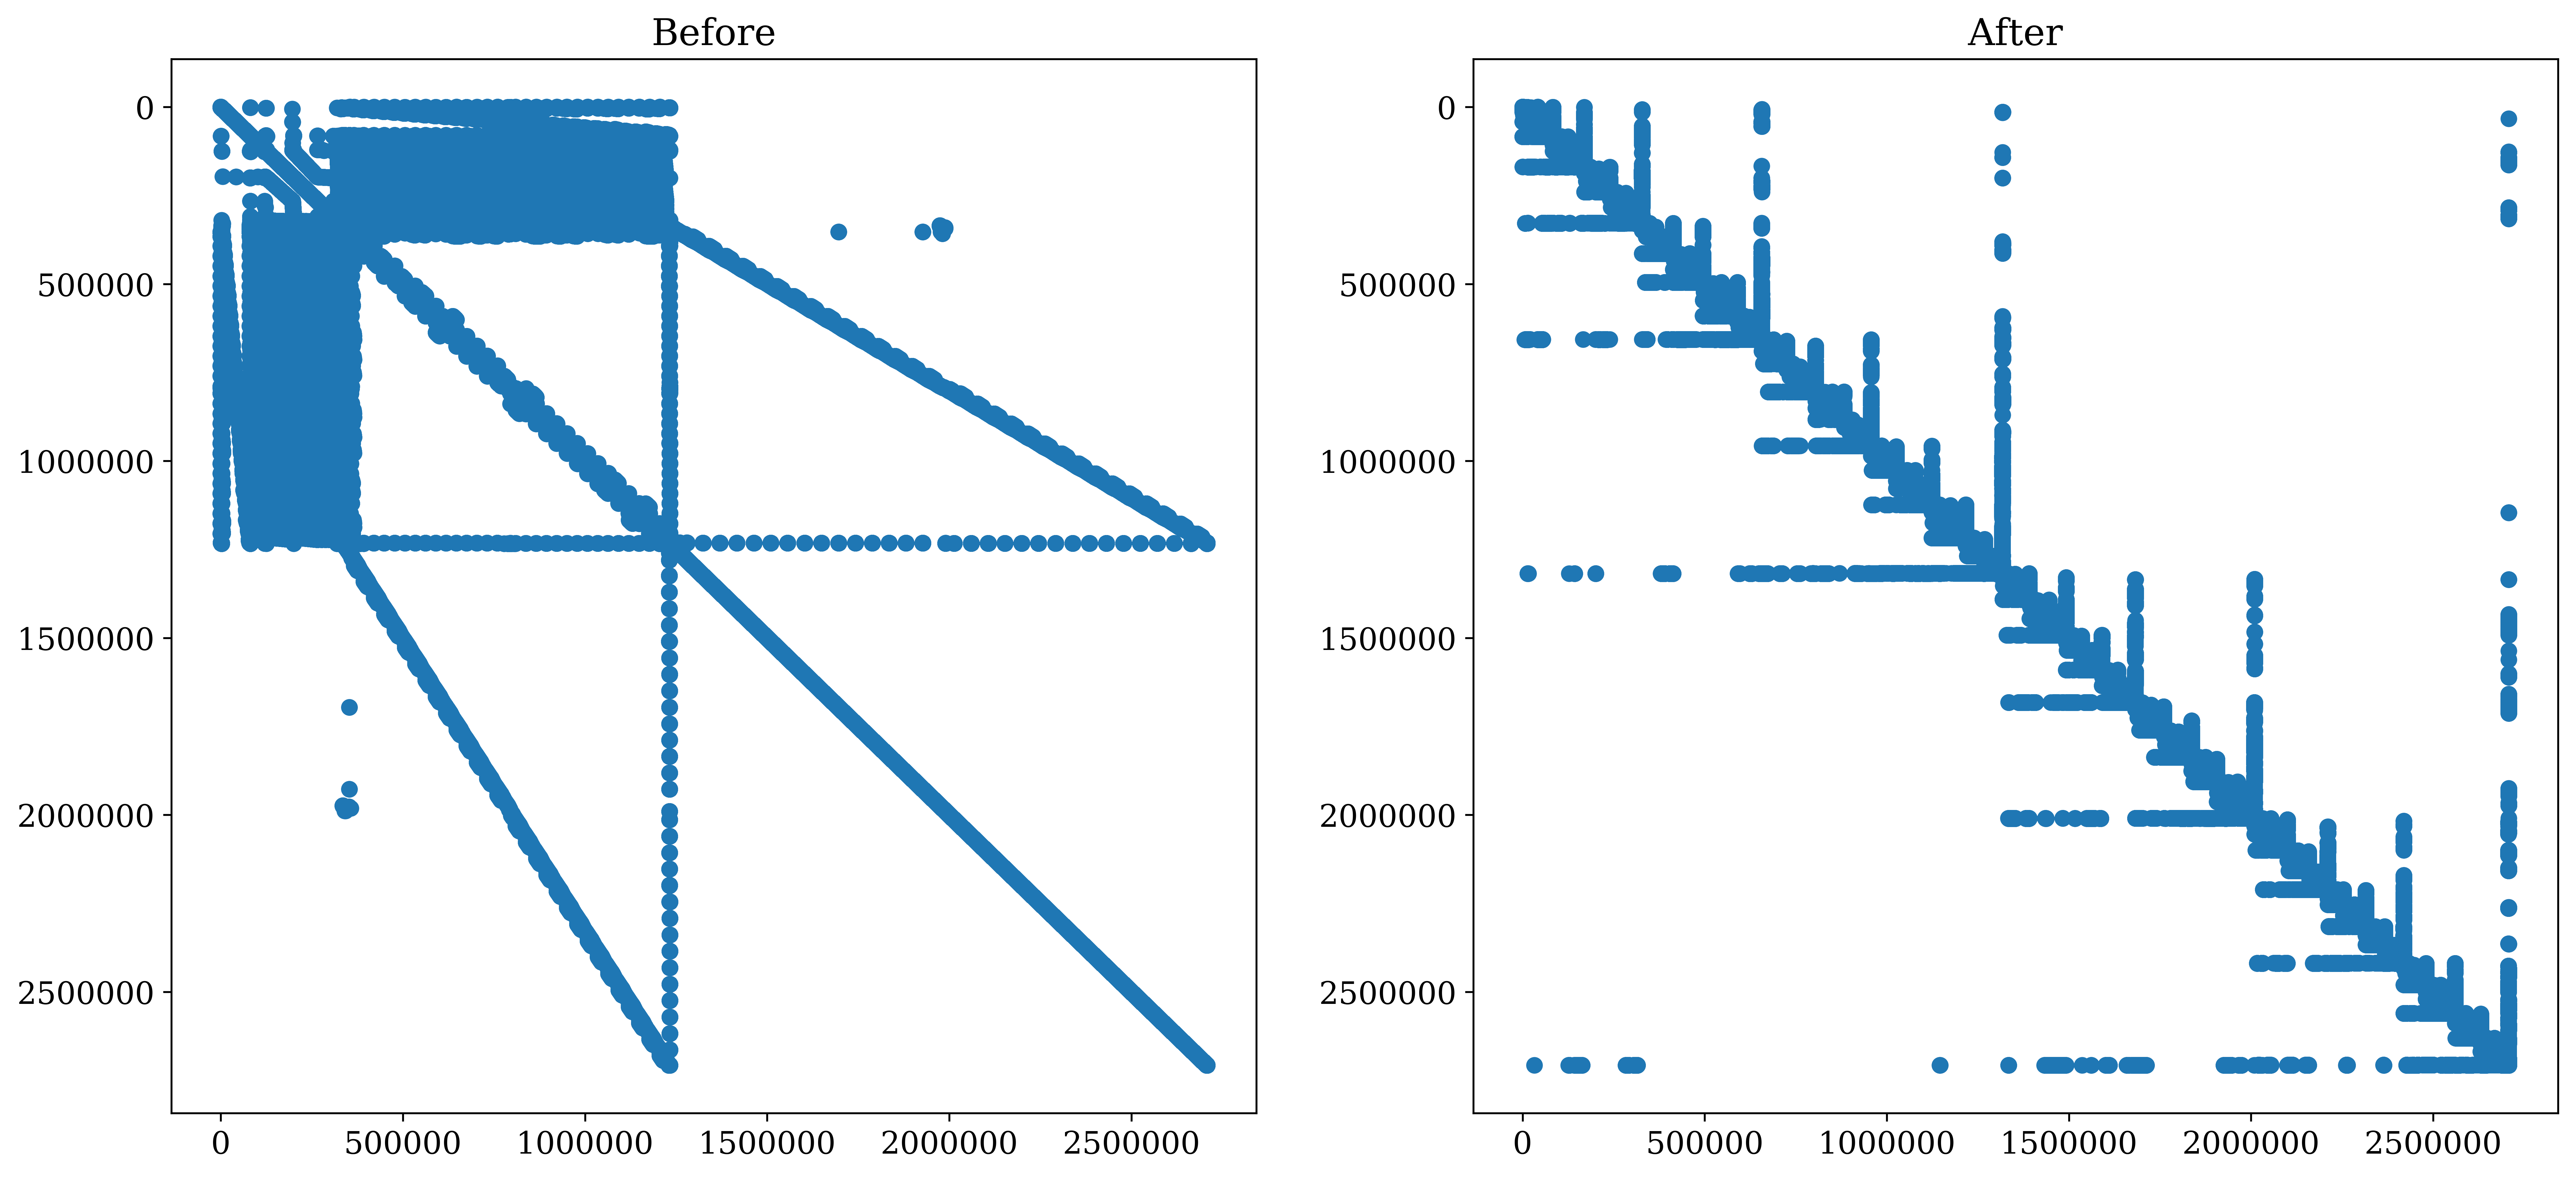
\includegraphics[width=1.00\textwidth]{figures/chapter-2/memchip-matrix-sparsity-pattern.png}
\caption{Sparsity structure of the matrix \textit{\textbf{memchip}} before and after fill-in reduction}
\label{fig:memchip-matrix-sparsity-pattern}
\end{figure}




As we can see, our model and the experiment show the same trend and the results are pretty much close to each other. However, our model takes into consideration only task parallelism whereas MUMPS exploits both data and task parallelism. Additionally, we have to mention that our model 1 works well only for relatively big sparse matrices. It can be quite inaccurate in case of small/skinny sparse systems. \\


In general, it is possible to refine our models and make them more accurate, using Bulk Synchronous Parallel (BSP) approach, for example. However, it will require to possess a real postordered elimination tree, extracted from a specific implementation of multifrontal method, together with information about supernodes sizes. We strongly believe the new enhanced model can explain the jagged strong scaling behavior of the MUMPS solver that we can observe in figure \ref{fig:model-1-vs-mumps}. But, this approach seems to be quite cumbersome and requires to delve into the source code of a particular library. It is needless to say that data can be retrieved only during run time and only after the analysis phase. This makes it less valuable and we can see that it is definitely a wrong way to go.\\


There are few important aspects to discuss at the end of the section. Numerical robustness is the main advantage of the multifrontal method. It does not require any preconditioner to solve a system of equations. As we discussed in the previous section, tuning a specific preconditioning algorithm can take a considerable amount of time, especially in case of our systems. As another advantage, the method (heavily) exploits matrix sparsity which lowers computational complexity up to $O(n^2)$. In case of massively huge matrices, the algorithm can utilize the secondary memory which sometimes is only one way to solve a system.\\


We can conclude, from the analysis above, the method has inherently bad scaling behavior and it is quite sensitive to a matrix structure. We will see later that it is almost impossible to predict the saturation point i.e. a point after which performance either drops or stays at the same level. We assume that scaling becomes better with growth of a matrix size. However, we cannot expect such behavior for small and medium systems.\\  


Secondly, we can see the algorithm requires many pre-processing steps to be done before numerical factorization phase. All these steps must run in parallel and be highly scalable. Apart from performance constrains of the steps, they must lead to wide and well balanced elimination trees which becomes crucial during the numerical phase.\\


Lastly, the algorithm can fail due to incorrect  working space prediction. As a results, factorization has to be restarted with some modification of input solver parameters.\\




\label{subseq:hybrid-method-description}

Nowadays, iterative methods is a common choice for solving sparse systems of linear equations because of their possible fast convergence and high parallel efficiency. However, application of such method always demands preconditioning of ill-conditioned systems to make methods converge to numerical accurate solutions. It can be clearly observed from table \ref{table:grs-matrix-set} that numerical integration of thermo-hydraulic simulations in \gls{athlet} entails solving such ill-conditioned systems  based on estimated condition numbers of matrices form \gls{grs} matrix set.\\


As the first step of the study, we tested various preconditioning algorithms together with their tuning parameters, mentioned in table \ref{table:preconditioners}, applied to \gls{grs} matrix set. \gls{gmres} was chosen as an iterative solver with values of relative and absolute convergence tolerances in the residual norm to be equal to $1E-8$ and $1E-4$, respectively. A coarse grid search was used with maximum 3 values for each tuning parameter starting from the default towards more accurate values in order to refine settings of each preconditioning algorithm. Testing results showed that none of them could lead to convergence for the entire set of matrices.\\


One can assume that a finer grid search can result in finding a suitable preconditioning algorithm with settings that can lead to convergence of \gls{gmres} solver for the entire set. However, it is important to point out the matrices were generated by running the most common \gls{grs} thermo-hydraulic test-scenarios and saving them somewhere during the time integration process. Hence, there is no guarantee that the settings found in such a way can always lead to convergence of \gls{gmres} solver in all time steps of any thermo-hydraulic simulation. Therefore, iterative methods may not satisfy \textit{robustness} criteria stated in chapter \ref{chapter:problem-statment} as a non-functional requirement to the time integration solver used in \gls{athlet}.\\


Taking into account the above reasoning, we have come to the conclusion that sparse direct methods is the best choice for our problem, in spite of the limited tree-task parallelism described in subsection \ref{subseq:direct-parallel-aspects}, because the methods stably result in numerical accurate solutions even in case of ill-conditioned linear systems. Hence, the next objective of the study is to find a suitable sparse direct method and its implementation, and adapt it for \gls{hw1} compute-cluster environment in terms of efficient parallel execution. \\

%\chapter{Configuration of a sparse linear solver}

	\section{Overview of Sparse Linear Solver Types} 

	
Next two subsections, i.e  \ref{subseq:part-2-iterative-solvers-theory} and \ref{subseq:part-2-direct-sparse-solvers-theory}, are organized as follows. The first part of each subsection contains a concise theory overview of a linear solver type. The second parts provide discussions of the main sources and means of parallelization of both iterative and direct sparse methods. The last part of each subsection focuses on issues related to numerical solution accuracy of a particular method type.\\
	
	%\chapter{Theoretical and parallelization aspects of iterative and direct sparse methods}

\label{subseq:overview-of-linear-solver-types}

\subsection{Iterative Methods}
\section{Iterative methods}
\label{subseq:iterative methods}
Iterative methods, especially Krylov subspace methods that we are going to discuss in this section, are well known for their relatively low storage requirements $O(nnz)$ and computation cost $O(N^2)$ in case of sparse linear systems of equations and good condition number. It turns out that sometimes it might be only one way to solve huge systems with millions unknowns.\\

The most well known methods are Conjugate Gradient (CG) for symmetric positive definite matrices, Minimal Residual Method (MINRES) for symmetric indefinite systems, Generalized Minimal Residual Method (GMRES) for non-symmetric systems of linear equations as well as different variants of GMRES such Biconjugate Gradient Method (BiCG), Biconjugate Gradient Stabilized Method (BiCGSTAB) and so on.\\

All Krylov methods solve a system of equation as a minimization problem. For example, the goal of CG algorithm is to minimize the energy functional $f(x) = 0.5 x^T A x - b^T x + c$, whereas, MINRES and GMRES tries to minimize residual norm $r_{j}$ for $x_{j}$ in a subspace. \\

%$j$th Krylov subspace $\mathcal{K}_{j}$. \\

The methods construct an approximate solution of a system as a linear combination of vectors $b$, $Ab$, $A^2b$, $A^3b$ and so on which defines the Krylov subspace. At each iteration we expand the subspace adding and evaluating a next vector in the combination.\\

Let's consider GMRES, as the most popular and general iterative solver, without preconditioning to just analyze its strong scaling behavior and potential problems. \\ 

As we mentioned above GMRES minimizes the residual norm in a subspace $U_m$.

\begin{equation} \label{eq:Gmres-1}
	\underset{x \in U_m}{min}||Ax - b||^2
\end{equation}

We can consider a solution vector $x$ in the subspace $U_m$ in a form $x=U_m y$. Thus, equation \ref{eq:Gmres-1} can be written as following:

\begin{equation} \label{eq:Gmres-2}
	\underset{x \in U_m}{min}||AU_m y - b||^2
\end{equation}

The most natural way to choose a proper subspace $U_m$ is the corresponding Krylov subspace $\mathcal{K}_m$ because it can be easily generated on the fly. However, decomposition of vector $x$ in that subspace can be a problem. Since the subspace $\mathcal{K}_m$ is spanned by the sequence of $b$, $Ab$, $A^2b$, ..., $A^{m-1}b$ and due to round-off error the sequence can become linear dependent. Therefore, we have to compute and use the orthonormal base of the given Krylov subspace. Saad and Schultz in their work \cite{sparse-la:gmrese-origin} used Arnoldi process for constructing an $l_2$-orthogonal basis. As the results equation \ref{eq:Gmres-2} can be written in the following form:  \\

\begin{equation} \label{eq:Gmres-3}
	\underset{x \in U_m}{min}||U_{m+1}H_{m+1,m} y - ||b||u_1||^2 = \\
	\underset{x \in U_m}{min}||H_{m+1,m} y - ||b||e_1||^2 
\end{equation}

where $H_m$ is an upper Hessenberg matrix. We can apply Givens rotation algorithm to compute $QR$ decomposition to convert $H_m$ to a strictly upper triangular matrix. Thus,

 
\begin{equation} \label{eq:Gmres-4}
	\underset{x \in K_m}{min}||Ax - b||^2 = \\
	\underset{x \in U_m}{min}||Q^TRy - ||b||e_1||^2 = \\
	\underset{x \in U_m}{min}||\Big(\begin{array}{c c}R_m \\ 0 \\\end{array}\Big) y - \Big(\begin{array}{c c} \tilde{b_m} \\ \tilde{b_{n-m}} \\\end{array}\Big)||^2
\end{equation}

Given \ref{eq:Gmres-4}, we can compute the solution as following:

\begin{equation} \label{eq:Gmres-5}
	R_m y = \tilde{b_m}
\end{equation}


\begin{equation} \label{eq:Gmres-6}
	x_m = U_m y  
\end{equation}

Because of large computational and storage costs, in case of evaluation of the full Krylov subspace, only small a subspace is computed, typically first 20 - 50 column vectors. Then the algorithm is restarted using the computed approximate solution as a initial guess for the next iteration.\\

We can see that some operations, for example \ref{eq:Gmres-6}, can be efficiently done in parallel. However, operatiopns like sparse triangular solve \ref{eq:Gmres-5} can introduce some effect on strong scaling behavior. Figure \ref{fig:sparse-triangular-solve-performance} shows strong scaling performance results of a sparse parallel triangular solver with a two dimensional matrix distribution. Performance considerations of the solver can be found in \cite{sparse-la:triangular-solve}.\\

\figpointer{\ref{fig:sparse-triangular-solve-performance}}

\begin{figure}[htpb]
  \centering
  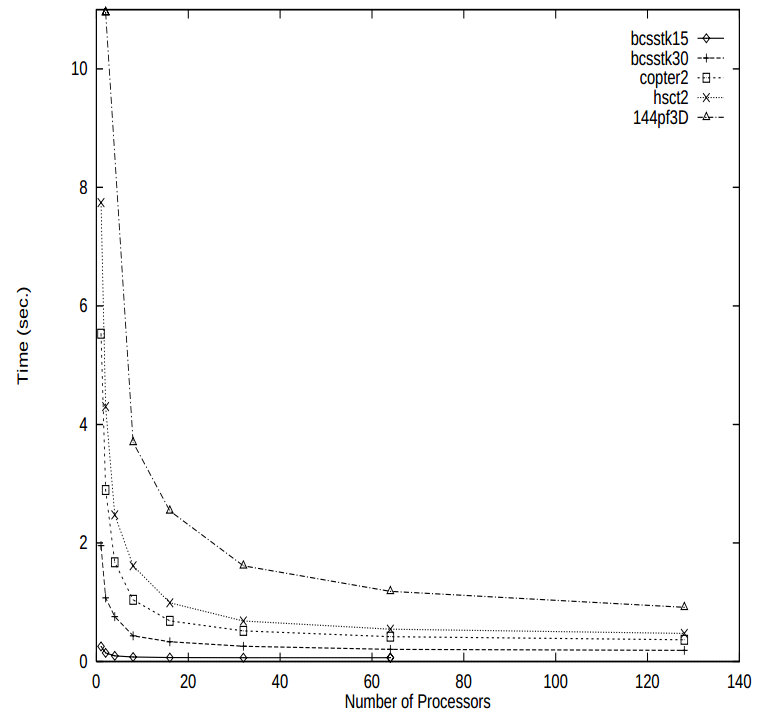
\includegraphics[width=0.5\textwidth]{figures/chapter-2/sparse-triangular-solve-performance.png}
\caption{Performance of sparse triangular solve \cite{sparse-la:triangular-solve}}
\label{fig:sparse-triangular-solve-performance}
\end{figure}


It is interesting to notice that performance of the triangular solver depends on a matrix sparsity structure as well as the matrix size. \\

Triangular solve \ref{eq:Gmres-5} can be computed in a single processor because matrix $R_m$ is usually small and depends on the number iterations before the restart. In this case the triangular solve can become a bottleneck again. \\

Figure \ref{fig:gmres-strong-scaling-speed-up} shows strong scaling performance results of the default GMRES solver from the PETSc library. The solver was set up without any preconditioner and 50 iterations as the restart. Additionally no stop criteria was specified except the maximum number iterations which was equal to 100. Four different matrices with different sparsity patterns were examined for the test. The information about the matrices is summarized in table \ref{table:matrix-info-1}. As we expected we can observe strong deviation of our test cases from the ideal speed-up when the number of processes exceeds 10.\\

It should be mentioned that parallelization overheads, introduced by such MPI operations as MPI\_Send, MPI\_Recv, MPI\_Allreduce, etc., also have their impact on performance of the algorithm.\\

\begin{table}[htpb]
\centering
\begin{tabular}{|c|c|c|c|}
\hline
Matrix Name & n       & nnz      & nnz / n \\ \hline
k3-18       & 1155955 & 7204723  & 6.2327  \\ \hline
k3-2        & 130101  & 13906057 & 6.0568  \\ \hline
cube-645    & 1000045 & 787997   & 13.9054 \\ \hline
cube-64     & 100657  & 1388993  & 13.7992 \\ \hline
\end{tabular}
\caption{Basic information about matrices used in figure \ref{fig:gmres-strong-scaling-speed-up}}
\label{table:matrix-info-1}
\end{table}

Other Krylov methods such as CG, for example, scales much better than GMRES. Because of the nature of the CG algorithm the next search direction can be found using a recurrent expression and the algorithms boils down to simple operations such as dot products and matrix vector multiplications. These operations can be easily parallelized and drop of performance comes only from MPI overheads. A quite comprehensive study about parallel CG algorithm performance can be found in \cite{sparse-la:cg}. The authors also introduced a deeply pipelined version of CG algorithm that scales even better due to overlapping the time-consuming global communication phase, induced by parallel dot product computations, with useful independent computations \cite{sparse-la:cg}.\\


\figpointer{\ref{fig:gmres-strong-scaling-speed-up}}
\begin{figure}[htpb]
  \centering
  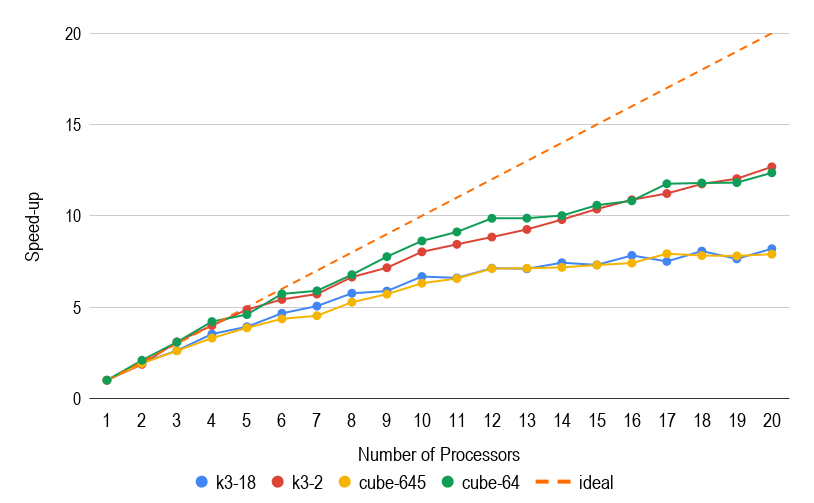
\includegraphics[width=0.8\textwidth]{figures/chapter-2/gmres-strong-scaling-speedup.png}
\caption{GMRES strong scaling speed-up}
\label{fig:gmres-strong-scaling-speed-up}
\end{figure}



% start discussion about preconditioning
The most important criteria of Krylov methods is convergence rate. The convergence rate of iterative methods strongly depends on a matrix and, in particular, on its condition number. For instance, equation \ref{eq:Gmres-7} shows dependence of the convergence rate from the matrix condition number. It can be clearly seen that a big condition number leads to very slow error reduction and, as the results, to huge number of iterations.\\

\begin{equation} \label{eq:Gmres-7}
	|| e^i ||_A \leq 2 ( \frac{\sqrt k - 1}{\sqrt k + 1} )^i || e^0 ||_A
\end{equation}

where $k = \frac{\lambda_{max}}{\lambda_{min}}$ - condition number of the corresponding matrix. \\

An obvious solution of such a problem is to reduce the condition number of the original system \ref{eq:slq}. A general method is to transform the original system in such a way that the conditional number of the transformed system gets significantly smaller. The transformation of \ref{eq:slq} can be done from the left side \ref{eq:pcn-1} or from the right one \ref{eq:pcn-2}.

\begin{equation} \label{eq:pcn-1}
	PAx = Pb
\end{equation}


\begin{equation} \label{eq:pcn-2}
	AP(P^{-1}x) = b
\end{equation}

where matrix $P$ is called preconditioner.\\


As an extreme example we can consider the inverse matrix $A^{-1}$ as the best preconditioner since it directly leads to the solution of the problem \ref{eq:slq} and, thus, it requires only one iteration. However, it is obvious that computation of inverse $A^{-1}$ is extremely expensive operation and it is not an objective of any iterative methods. That example helps understand and set requirements for preconditioners, namely:

\begin{enumerate}
	\item cheap to compute e.g. a 5-10 iterations of the corresponding Krylov solver
	\item should lead to a small conditioner number of the transposed system
	\item should be sparse, otherwise storage requirements will considerably increase
\end{enumerate}


There exist numerous techniques to compute preconditioners given a matrix $A$ e.g. (point) Jacobi, Block-Jacobi, incomplete $LU$ decomposition (ILU), multilevel ILU (ILU(p)), threshold ILU (ILUT), incomplete Cholesky factorization (IC), sparse approximate inverse (SPAI), multigrid as a preconditioner, etc. Almost all methods listed above have some tuning parameters which allow to get a better preconditioner i.e. a smaller condition number of the transformed system. However, it usually leads to increase of computational and storage costs. \\

Some methods can works particularly well for matrices derived from certain PDEs e.g. Poisson, Navier\-Stokes, etc. problems discretized using the cartesian grid. However sometimes it can take a considerable amount of time to choice right parameters for a certain preconditioning algorithm. It can become a challenge to fulfill all requirements 1, 2, 3 mentioned above. \\

Table \todo{Table with comparisons of different preconditioning for our test cases}

Table [] shows results of different preconditioning algorithms application to our test case. It can be seen that some algorithms failed even after tuning. \\

It interesting to notice that \citeauthor{wsmp} came to approximately the same results working on their set of matrices in their work \cite{wsmp}. They observed that preconditioned iterative solvers worked efficiently only for 2 out 5 cases in contrast to direct sparse solvers.\\

We can summarize that it is vital to perform careful parameter tuning of any preconditioning algorithms combining results from [table] and \cite{wsmp}. In general the  search can take a considerable amount of time. Moreover, it becomes impractical for time integration problems where topology of an underlying problem and, as the results, the computational mesh, discretization, Jacobian matrix can be changed over time of a simulation. It is obvious that parameters chosen for a particular time step can become not optimal for consecutive steps and, at the end, it can lead to divergence. If divergence happens at any time step the entire time integration algorithm fails and the simulation has to be restarted with different preconditioning parameters or with a different preconditioning algorithm.\\

By and large we come to a conclusion that preconditioned iterative solvers are not robust and thus cannot fully fulfill requirements listed in section \ref{chapter:solver configuration}.\\

% maybe above we have to mention inderect memory access and its effect on performance
 

\subsection{Direct Sparse Methods}
\section{Direct sparse methods}
\label{subseq:sparse methods}

Direct sparse methods combine main advantages of direct and iterative methods i.e. numerical robustness and usage of sparsity structures. As a results, there is no need for preconditioning and the computation complexity is $O(n^2)$ \cite{complexity-of-spdm}. The problem is that storage cost can significantly increase during factorization i.e. the inverse of a sparse matrix can be sufficiently dense. To reduce storage space of $LU$ decomposition this group of methods performs fill-in reduction reodering as a pre-processing step before actual factorization. If storage space is still huge even after fill-in reduction reodering out-of core factorization can be used where partial results are stored in the secondary memory. \\

The most widely known sparse direct method is multifrontal method introduced by \citeauthor{mult-frontal-original:1} in their work \cite{mult-frontal-original:1}. Multifrontal method is an improved extension of a frontal method \cite{frontal-original} that can compute independent fronts in parallel. A front, or also called frontal matrix, can be considered as small dense matrix which is a result of Gaussian Elimination for a particular column. The algorithm, in fact, is as a variant of Gaussian Elimination process. There also exist left-looking and right-looking sparse direct methods. The difference between all of them is explained and can be found in \cite{elimination-tree}.\\


In order to understand and analyze strong scaling behavior of the algorithm we have to briefly discuss the theory of the method. For simplicity we will assume that matrix $A$ is real symmetric and $LU$ decomposition boils down to the Cholesky factorization \ref{eq:chol-1}. It allows us to focus on the Cholesky factor $L$ and its sparsity pattern only.

\begin{equation} \label{eq:chol-1}
	A = LDL^T
\end{equation}

The algorithm usually starts with symbolic factorization to predict sparsity pattern of $L$. Once it is done the corresponding elimination tree has to be constructed.\\

\figpointer{\ref{fig:sparsity-pattern-example-mm}}

\begin{figure}[htpb]
  \centering
  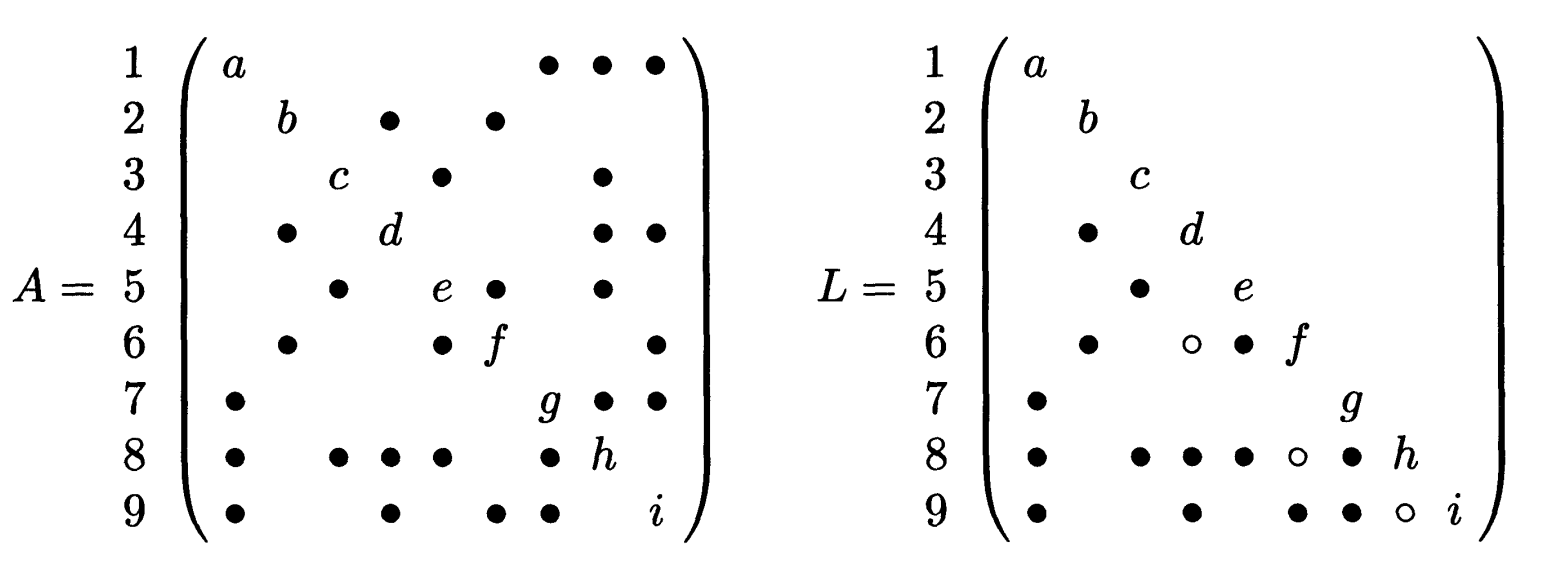
\includegraphics[width=0.9\textwidth]{figures/chapter-2/sparsity-pattern-example-mm.png}
\caption{An example of a sparse matrix and its Cholesky factor \cite{mult-frontal-original:2}}
\label{fig:sparsity-pattern-example-mm}
\end{figure}


Figure \ref{fig:sparsity-pattern-example-mm} shows an illustrative example of a sparse matrix and its Cholesky factor from \cite{mult-frontal-original:2}. The solid circles represent original non-zero elements whereas hollow ones define fill-in factors of $L$. \\


The elimination tree is a crucial part of the method. It can be considered as a structure of $n$ nodes that node $p$ is the parent of $j$ if and only if it satisfies equation \ref{eq:elimination-tree-1}. It is worth pointing out the definition \ref{eq:elimination-tree-1} is not only one possible and one can define a strucutre of an elimination tree in a different way as well. As an example one can find a definition of a general assembly tree in \cite{mult-frontal-original:2} proposed by \citeauthor{mult-frontal-original:2}.\\

\begin{equation} \label{eq:elimination-tree-1}
	p = min(i > j | l_{ij} \neq 0)
\end{equation}


It is important to notice that node $p$ represents elimination process of the corresponding column $p$ of matrix $A$ as well as all dependencies of column $p$ factorization on the results of its descendants.\\


Given definition \ref{eq:elimination-tree-1} we can build the corresponding elimination tree as it is shown in figure \ref{fig:elimination-tree-mm}.\\


\figpointer{\ref{fig:elimination-tree-mm}}

\begin{figure}[htpb]
  \centering
  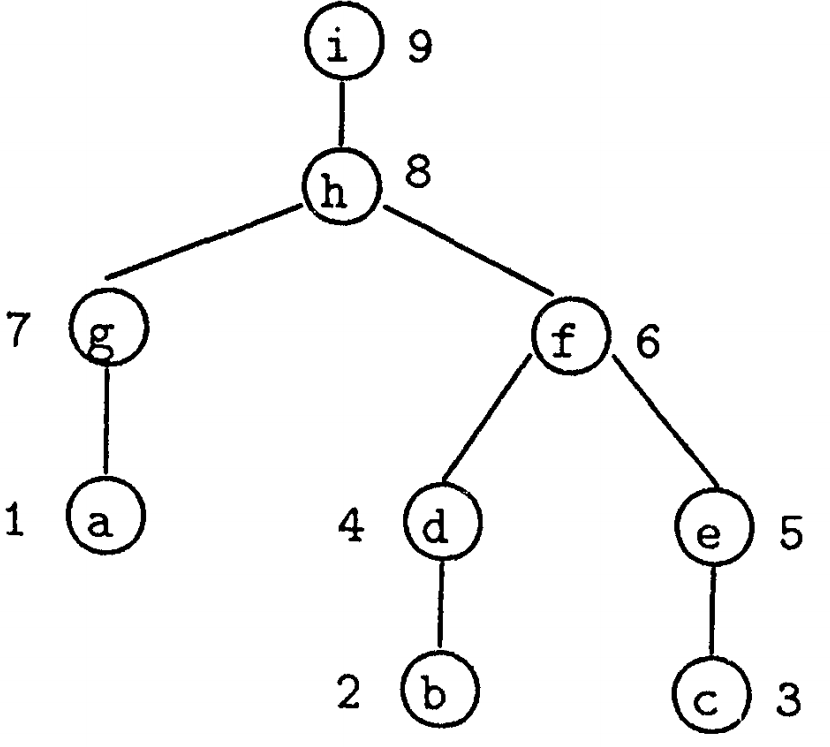
\includegraphics[width=0.45\textwidth]{figures/chapter-2/elimination-tree-mm.png}
\caption{The elimination tree for the matrix example in Figure \ref{fig:sparsity-pattern-example-mm}
 \cite{mult-frontal-original:2}}
\label{fig:elimination-tree-mm}
\end{figure}


The fundamental idea of multifrontal method spins around frontal and update matrices. A frontal matrix is used to perform Gaussian Elimination for a specific column $j$. It is a sum of a frame and update matrices as it can be seen from equation \ref{eq:mm-1}\\.

\begin{equation} \label{eq:mm-1}
	F_{j} = Fr_{j} + \hat{U_{j}} = \begin{bmatrix}a_{j,j} & a_{j,i_1} & a_{j,i_2} & \dots & a_{j,i_r} \\
a_{i_1,j} \\
a_{i_1,j} \\
\vdots & & & 0\\
a_{i_r,j} \\
\end{bmatrix} + \hat{U_{j}}
\end{equation}

where $i_{0}$, $i_{1}$, \dots , $i_{r}$ are the row subscripts of non-zeros in $L_{*j}$ with $i_{0} = j$ and $r$ is number of off-diagonal non-zero elements.\\

The frame matrix $Fr_{j}$ is filed with zeros except the first row and column. The first row and column contain non-zeros elements of the $j$th row and column of the original matrix $A$. Because we consider matrix $A$ to be symmetric the frame matrix is square and symmetric as well.\\

In order to describe parts of the elimination tree we will use the notation $T[j]$ to represent all descendants of the node $j$ in the tree and node $j$ itself. In this way we can define the update matrix $\hat{U_{j}}$ as following:\\

\begin{equation} \label{eq:mm-2}
	\hat{U_{j}} = - \sum_{k \in T[j] -{j}}  \begin{bmatrix}
l_{j,k} \\
l_{i_1,k} \\
\vdots \\
l_{i_1,k} \\
\end{bmatrix} \begin{bmatrix}
l_{j,k} & l_{i_1,k} & \dots & l_{i_1,k}
\end{bmatrix} 
\end{equation}


The update matrix $\hat{U_{j}}$ is, in fact, can be considered as the second term of the Schur complement i.e. update contributions from already factorized columns of $A$.\\

The subscript $k$ represents descendant columns of node $j$. Thus we include and consider only those elements of descendant columns which correspond to the non-zero pattern of the $j$th column that we are currently factorizing.\\

Let's consider the partial factorization of 2-by-2 block dense matrix to better understand essence of update matrix $\hat{U_{j}}$.\\


\begin{equation} \label{eq:mm-3}
A = \begin{bmatrix}
B & V^{T} \\
V & C
\end{bmatrix} 
= 
\begin{bmatrix}
L_{B} & 0 \\
VL^{-T}_{B} & I
\end{bmatrix}
\begin{bmatrix}
I & 0 \\
0 & C - VB^{-1}V^{T}
\end{bmatrix} 
\begin{bmatrix}
L^{T}_{B} & L^{-1}_{B}V^{T} \\
0 & I
\end{bmatrix} 
\end{equation}

Again we assume that $B$ has already been factorized and can be expressed as:

\begin{equation} \label{eq:mm-4}
	B = L_{B}L^{T}_{B}
\end{equation}

The Schur complement from equation \ref{eq:mm-3} can be viewed as the original sub-matrix $C$ and update $-VB^{-1}V^{T}$. It can be written in a vector form as well:

\begin{equation} \label{eq:mm-5}
	-VB^{-1}V^{T} = -(VL^{-T}_{B})(L^{-1}_{B}V^{T}) = - \sum_{k=1}^{j-1}  \begin{bmatrix}
l_{j,k} \\
\vdots \\
l_{n,k} \\
\end{bmatrix} \begin{bmatrix}
l_{j,k} & \dots & l_{n,k}
\end{bmatrix} 
\end{equation}

As it can be easily seen that equations \ref{eq:mm-5} and \ref{eq:mm-2} are identical. The difference is that equation \ref{eq:mm-2} exploits sparsity of the corresponding row and column of $L$ and thus masks unnecessary information. \\

% both eqautions show that the update matrix aggregate all previous information done and in case of the ,ultifrontal methods it means that we aggregate all information from descendants

% Therefore, we can express Uy as an aggregate of outer- product updates from columns in T[Cl],..., T[cs]. 

We can also notice from equation \ref{eq:mm-3} that the frame matrix $Fr_{j}$ corresponds to the block matrix $C$ and brings information from the original matrix $A$ whereas matrix $\hat{U_{j}}$ adds information about the columns that have already been factorized.\\

As soon as the frontal matrix $F_{j}$ is assembled i.e. we have the complete update of column $j$, we can perform elimination of the first column and get non-zero entries of factor column $L_{*j}$.\\

Let's denote $\hat{F_{j}}$ as a result of the first column factorization of the frontal matrix $F_{j}$. Then we can express the results as following:\\


\begin{equation} \label{eq:mm-6}
\hat{F_{j}} = \begin{bmatrix}
l_{j,j} & \dots & 0 \\
\vdots & I \\
l_{i_{r},j} \\
\end{bmatrix} 
\begin{bmatrix}
1 & \dots & 0 \\
\vdots & U_{j} \\
0 \\
\end{bmatrix} 
\begin{bmatrix}
l_{j,j} & \dots & l_{i_{r},j} \\
\vdots & I \\
0 \\
\end{bmatrix} 
\end{equation}

where sub-matrix $U_{j}$ represents the full update from all descendants of node $j$ and node $j$ itself. Equation \ref{eq:mm-7} express the sub-matrix $U_{j}$ in a vector form.\\

\begin{equation} \label{eq:mm-7}
\hat{U_{j}} = - \sum_{k \in T[j]}  \begin{bmatrix}
l_{i_1,k} \\
\vdots \\
l_{i_1,k} \\
\end{bmatrix} \begin{bmatrix}
l_{i_1,k} & \dots & l_{i_1,k}
\end{bmatrix}
\end{equation}

Together with the frontal $F_{j}$ and update $\hat{U_j}$ matrices, the update column matrix $U_{j}$ (also called contribution matrices) forms the key concepts of the multifrontal method. To consider the importance of sub-matrix $U_{j}$ let's consider and example illustrated in Figure \ref{fig:information-float}.\\

\figpointer{\ref{fig:information-float}}
\begin{figure}[htpb]
  \centering
  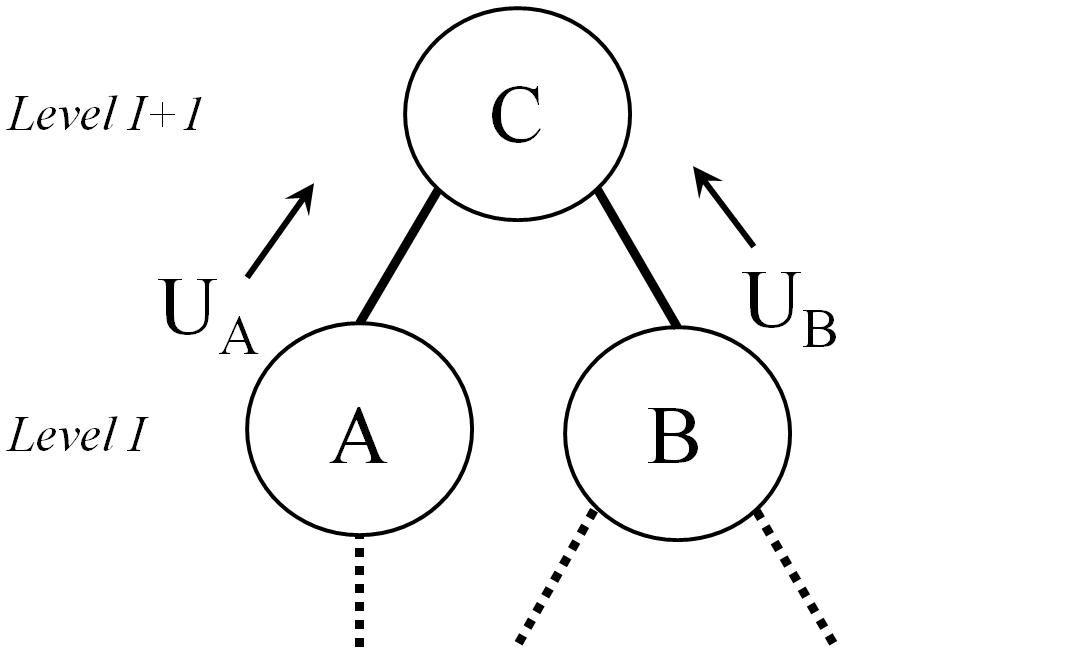
\includegraphics[width=0.45\textwidth]{figures/chapter-2/information-flow.png}
\caption{Information flow of the multifrontal method}
\label{fig:information-float}
\end{figure}


We assume that factorization of columns A and B have already been done and corresponding contribution matrices $U_{A}$ and $U_{B}$ have been computed. From equation \ref{eq:mm-7} we have already known that both $U_{A}$ and $U_{B}$ contain the full updates of all their descendants including updates from factorization of columns $A$ and $B$ as well. Therefore update column matrices $U_{A}$ and $U_{B}$ have already got all necessary information to construct update matrix $\hat{U_{C}}$. The detailed proof and careful explanation can be found in \cite{mult-frontal-original:2}.\\


It might happen that we do not need all rows and columns of $U_{A}$ and $U_{B}$ i.e. we need only some subset of them, because of sparsity of column $C$ . It is also important to place all necessary rows and columns of matrices $U_{A}$ and $U_{B}$ in a right place within matrix $\hat{U_{C}}$. For that reason, an additional matrix operation, called \textbf{\textit{extend-add}}, must be introduced.\\

Let's consider an example from \cite{mult-frontal-original:2} of an extend-add operation for 2-by-2 matrices $R$ and $S$ which correspond to the indices ${5,8}$ and ${5,9}$ of some matrix $B$, respectively.\\

\begin{equation}
R = \begin{bmatrix}
p & q \\
u & v \\
\end{bmatrix} 
,
\:
S = \begin{bmatrix}
w & x \\
y & z \\
\end{bmatrix} 
\end{equation}

The result of the operation is going to be a 3-by-3 $K$ matrix which looks as following:\\

\begin{equation} \label{eq:mm-8}
K = R \extendadd S = \begin{bmatrix}
p & q & 0 \\
u & v & 0 \\
0 & 0 & 0 \\
\end{bmatrix} 
+
\begin{bmatrix}
w & 0 & x \\
0 & 0 & 0 \\
y & 0 & z \\
\end{bmatrix} 
=
\begin{bmatrix}
p + w & q & x \\
u & v & 0 \\
y & 0 & z \\
\end{bmatrix} 
\end{equation}

Hence we can express formation of the frontal matrix $F_{j}$ using the extend-add operation and all direct children of node $j$ in the following way:


\begin{equation} \label{eq:mm-9}
	F_{j} = \begin{bmatrix}a_{j,j} & a_{j,i_1} & a_{j,i_2} & \dots & a_{j,i_r} \\
a_{i_1,j} \\
a_{i_1,j} \\
\vdots & & & 0\\
a_{i_r,j} \\
\end{bmatrix} \extendadd U_{c_1} \extendadd \dots \extendadd U_{c_s} 
\end{equation}

where $c_{1}, \: c_{2}, \: \dots \: c_{n}$ are indices of direct children of the node $j$.\\

Now it can be clearly seen that the resultant frontal matrix $F_{j}$ is a small dense one and it can be efficiently computed using BLAS level 3 subroutines.\\

After factorization we have to build the contribution matrix $U_{j}$ i.e. add columns and rows of $U_{c_1}, \:, U_{c_2}, \: \dots, U_{c_s}$ to $U_{j}$ that have not been used in factorization of $F_{j}$ due to sparsity of column $j$. After that we can continue to move up along the tree. 
The complete update matrices grow in size as we move to the top of the tree. Therefore they have to be stored in a sparse matrix format to stay within memory constrains of the computer.\\


Another important aspect is storage and manipulation of frontal and contribution matrices. Sometimes we have to store contribution matrices produced in previous steps into some temporary buffer and efficiently retrieve them later during factorization. This can require some matrix re-ordering. In case of symmetric matrices, one can apply postordering on a tree to be able to use the stack data structure to alleviate the process of contribution matrix manipulations during factorization. A tree postordering is based on topological ordering and it has been proven that it is equivalent to the original matrix ordering and thus leads to the same filled graph \cite{mult-frontal-original:2}. \todo{sentence refactoring} We refer to the original matrix ordering as the ordering received from fill-in reduction operation.\\


A tree postordering means that a node is ordered before its parent and, additionally, nodes in each subtree are numbered consecutively. Figure \ref{fig:mm-matrix-postordering} shows an example of posrordering applied to the elimination tree of the matrix from figure \ref{fig:sparsity-pattern-example-mm}. The results of this can be see in figure \ref{fig:mm-contrib-matrix-manipulation} where consecutive \textit{push} and \textit{pop} operations are efficiently used during factorization and thus simplify the program logic.\\


\figpointer{\ref{fig:mm-matrix-postordering}}
\begin{figure}[htpb]
  \centering
  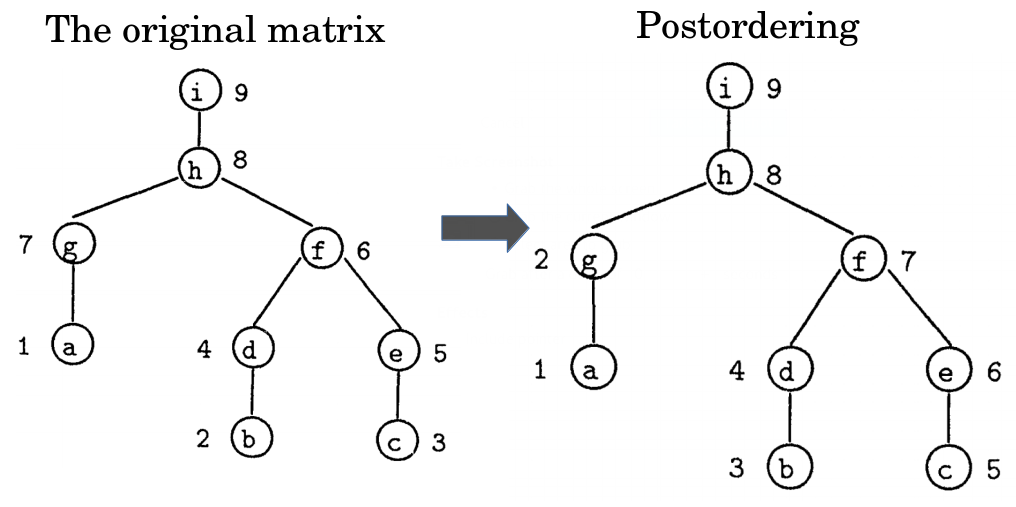
\includegraphics[width=0.75\textwidth]{figures/chapter-2/elimination-tree-mm-postordering.png}
\caption{An example of matrix postordering from \cite{mult-frontal-original:2}}
\label{fig:mm-matrix-postordering}
\end{figure}


\figpointer{\ref{fig:mm-contrib-matrix-manipulation}}
\begin{figure}[htpb]
  \centering
  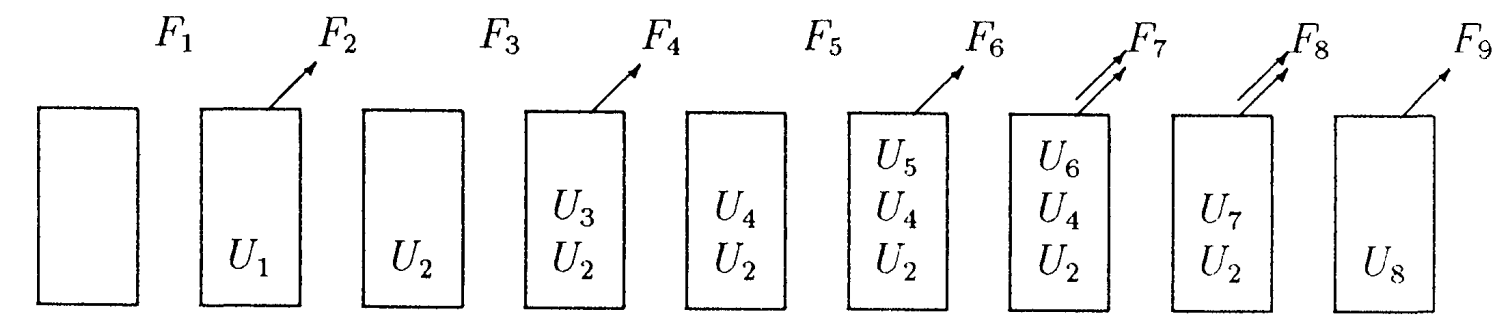
\includegraphics[width=0.75\textwidth]{figures/chapter-2/mm-contrib-matrix-manipulation.png}
\caption{The stack contents for the postordering \cite{mult-frontal-original:2}}
\label{fig:mm-contrib-matrix-manipulation}
\end{figure}


We can see the algorithm requires to perform some preprocessing steps in order to estimate the size of working space for matrix manipulations. If the working space has not been predicted correctly the algorithm will terminate during factorization. Additionally it can happen that even with the correct estimation we can be run out of space in the main memory, in case of huge sparse matrices. This fact can require to use the secondary memory and, as a result, the execution time will increase significantly. Therefore, different optimal postordering schemes have been proposed which allow to shrink the amount of space needed during factorization \cite{mm:optimal-tree-postordering} \cite{mm:elimination-tree-rotations}. Some schemes, for example elimination tree rotations \cite{mm:elimination-tree-rotations}, can lead to deep and unbalanced trees which might have their negative effect on task parallelism as we will see later.\\


In general, the estimation of working space can be tricky due to pivoting. Because pivoting happens only during the numerical factorization it is not always possible to estimate enough space correctly beforehand. There exist some heuristics which allow to use some numerical matrix information during symbolic factorization to better predict the amount of required space \cite{wsmp:direct-solution-of-general-system}.\\



It can be clearly observed the method consists of three distinct phases, namely: analysis, numerical factorization and solution. The analysis phase includes all pre-processing steps that have been discussed above i.e. fill-in reduction, postordering, symbolic factorization, building elimination tree an so on. During the numerical factorization phase the $L$ and $D$ (or $U$) parts of a matrix $A$ are computed based on sequence of dense factorization on frontal matrices. At the solution step, the solution vector $x$ is computed by means of backward and forward substitutions (equations \ref{eq:lu} and \ref{eq:bk}).\\


% supernodal
In practice, an improved version of multifrontal method, called supernodal method, is used. The idea of the supernodal method is to shrink the final elimination tree by grouping some particular nodes/columns in one computational unit. As a result, more useful floating point operations per memory access can be performed by eliminating few columns at once within the same frontal matrix.\\


% FOR PRESENTATION: Working on supernodes instead of individual variables is essential in order to speed-up the computations and use high-level BLAS [72] (Basic Linear Algebra Subprograms): supernodes lead to a higher flops to memory access ratio, and this allows a better usage of memory hierarchy and better performance thanks to the blocking techniques used in BLAS routines.



A supernode is formed by a set of contiguous columns with identical off-diagonal sparsity structure forms. Thus, a supernode has few important properties. Firstly, it can be expressed as a set of indices, namely: $\{j, \: j+1, \: \dots, \:j + t\}$, where node $j + k$ is	parent of $j + k - 1$ in the elimination tree. Secondly, the size of the supernodal frontal matrix is equal to the frontal matrix of the $j$th column within a supernode. As an example, Figure \ref{fig:supernodal-method-postordering-and-etree} shows a postordered matrix $A$ and its Cholesky factor $L$ as well as the corresponding supernodal elimination tree.


\figpointer{\ref{fig:supernodal-method-postordering-and-etree}}

\begin{figure}[htpb]
  \centering
  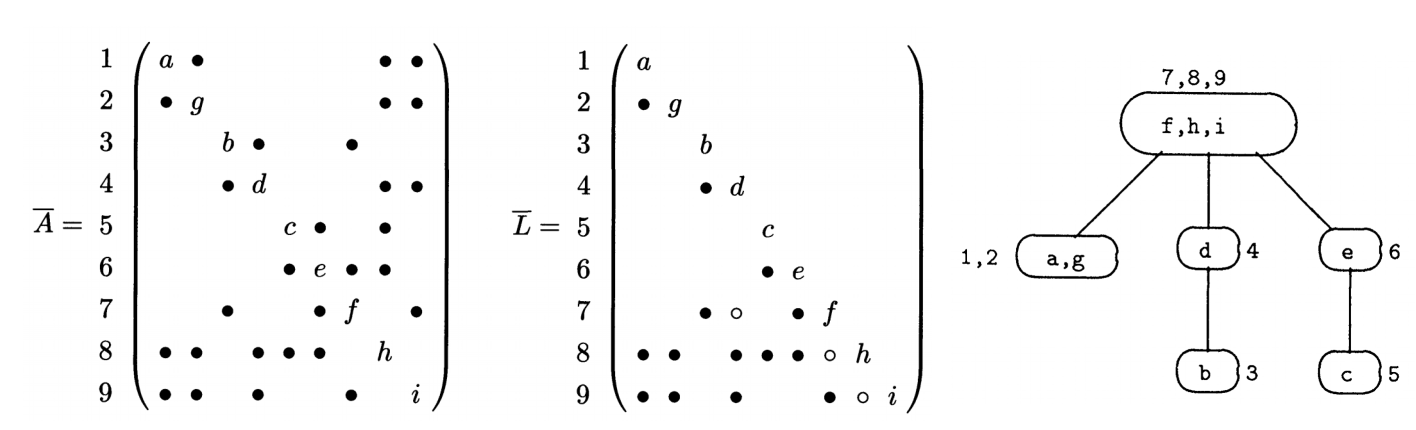
\includegraphics[width=1.0\textwidth]{figures/chapter-2/supernodal-method-postordering-and-etree.png}
\caption{An example of a supernodal elimination tree \cite{mult-frontal-original:2}}
\label{fig:supernodal-method-postordering-and-etree}
\end{figure}
 
 
Equation \ref{eq:mm-10} expresses the building process of a frontal matrix of a supernode. In contrast to \ref{eq:mm-9}, the frame matrix $\mathcal{F}_{j}$ contains more dense rows and columns. As before, we use \textit{extend-add} operation to get the full block update from children contribution matrices.\\


\todo{check grammar}
It should be mentioned there exist more sophisticated variants of supernodes. Most of the time, it intends to improve efficiency of the algorithm. \citeauthor{mult-frontal-original:2} pointed out that supernodes could be defined without using the contiguous constrains \cite{mult-frontal-original:2}. On another hand, \citeauthor{complexity-of-spdm} defines supernodes corresponded to separators from the nested dissection step  \cite{complexity-of-spdm} which was used for fill-in reduction.\\



 \begin{equation} \label{eq:mm-10}
	\mathcal{F}_{j} = \begin{bmatrix}a_{j,j} & a_{j,j+1} & \dots & a_{j,j+t}  & a_{j,i_1} & \dots & a_{j,i_r} \\
a_{j+1,j} & a_{j+1,j+1} & \dots & a_{j+1,j+t}  & a_{j+1,i_1} & \dots & a_{j+1,i_r} \\
\vdots & \vdots & \dots & \vdots \\
a_{j+t,j}  & a_{j+t,j+1} & \dots & a_{j+t,j+t}  & a_{j+t,i_1} & \dots & a_{j+t,i_r} \\
a_{i_1,j} & a_{i_1,j+1} & \dots & a_{i_1,j+t} \\
\vdots & \vdots & \dots & \vdots  & & 0\\ 
a_{i_r,j} & a_{i_r,j+1} & \dots & a_{i_r,j+t} \\
\end{bmatrix} \extendadd U_{c_1} \extendadd \dots \extendadd U_{c_s} 
\end{equation}


Up to this point we have already seen all key concepts of the multifrontal method and discussed how the algorithm works. We will move to the discussion of parallelization of the method. \\


The elimination tree, in fact, represents dependencies among columns. Conversely, the tree also shows independent steps of elimination process. Hence the tree forms independent problems that can be executed in parallel. Task parallelism is the main and primary source the algorithm parallelisation. Figure \ref{fig:elimination-tree-mm-parallel-steps} shows task parallelism, for the example given in Figure \ref{fig:supernodal-method-postordering-and-etree}, where each color represents a set concurrent tasks.\\


\figpointer{\ref{fig:elimination-tree-mm-parallel-steps}}

\begin{figure}[htpb]
  \centering
  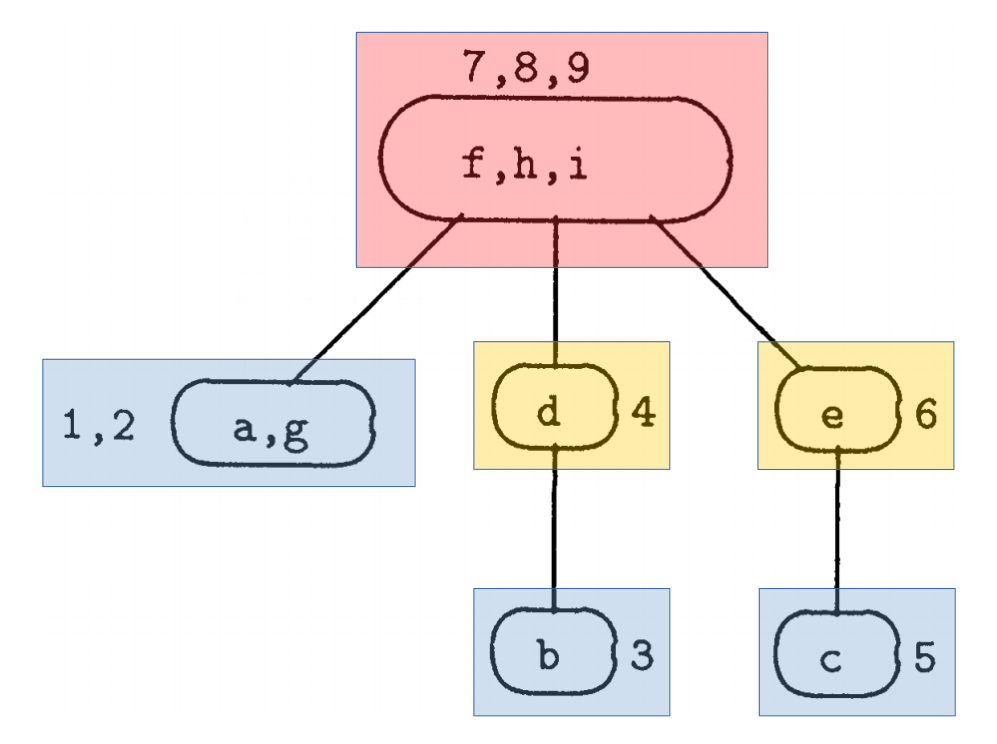
\includegraphics[width=0.5\textwidth]{figures/chapter-2/elimination-tree-parallel.png}
\caption{Parallel steps of the multifrontal method based on the example in Figures \ref{fig:supernodal-method-postordering-and-etree}}
\label{fig:elimination-tree-mm-parallel-steps}
\end{figure}


For example, nodes on separate branches of the tree are totally independent and can processed in parallel. However, as soon as at least two branches run into the same node it forms a dependency and we have to wait all contribution matrices of its children and cannot proceed further.\\ 


We can observe the amount of task parallelism is rapidly decreasing while moving towards the root along the tree. Once we reach the root of the tree the algorithm becomes totally sequential. This fact can play the significant role in strong scaling behavior of the method.\\


We developed two simple models based on perfectly balanced binary trees to better understand strong scaling of the algorithm. The main concept of the models is so-called cost per level or cost per node. This idea is similar to the recursion trees in \cite{recursion-tree} which explains and computes complexity of recurrent algorithms.\\


Figure \ref{fig:mm-parallel-model-tree-linear} represents the first model where we keep the same cost per level whereas the second model (Figure \ref{fig:mm-parallel-model-tree-quadratic}) simulates quadratic cost decay from level to level. Additionally we assume that computational cost distributed uniformly between nodes at the same level for both models.\\


\figpointer{\ref{fig:mm-parallel-model-tree}}
\begin{figure}
\centering
	\begin{tabular}{cc}
			\subfloat[Model 1: equal cost per level]{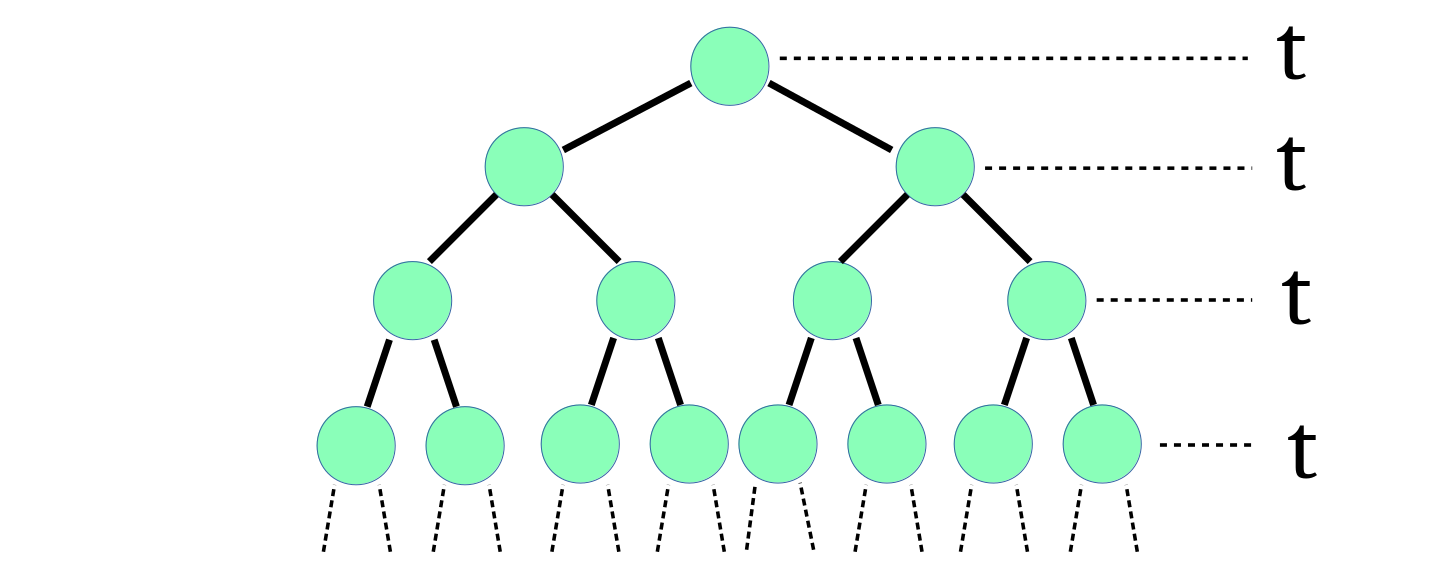
\includegraphics[width=0.5\textwidth]{figures/chapter-2/mm-parallel-model-tree-1.png} \label{fig:mm-parallel-model-tree-linear}} & 
		\subfloat[Model 2: quadratically decreasing cost per level]{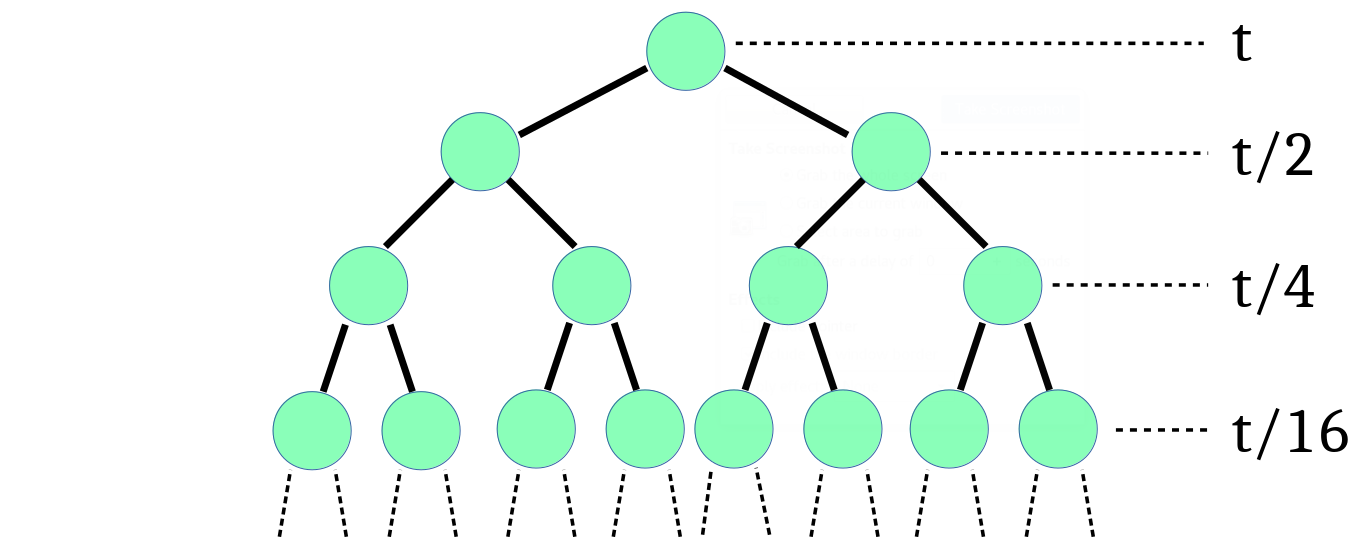
\includegraphics[width=0.5\textwidth]{figures/chapter-2/mm-parallel-model-tree-2.png} \label{fig:mm-parallel-model-tree-quadratic}} \\
	\end{tabular}
	\caption{Simple parallel models of the multifrontal method}
	\label{fig:mm-parallel-model-tree}
\end{figure}

\todo{sentence refactoring}
We have to say that our models mimic only numerical factorization and do not include time spent on any per-processing steps, for example, fill-in reduction reodering. A cost per level can be interpreted in different ways e.g. increase of partial factorization time due to growth of frontal matrices in size, time increase spent on numerical pivoting, increase of MPI communication overheads due to growth of contribution matrices, etc. It should be mentioned that real computer implementations of the multifrontal algorithm (MUMPS, SuperLU, etc.) are quite sophisticated in many aspects and our models do not have any intention to analyze performance of a particular package. Instead the objective of these models is to show possible strong scaling behavior and possible bottlenecks. \\


We will consider only task parallelism at the beginning to a first approximation and later we will discuss how additional data parallelism can affect algorithm performance.\\

% assumtion that cost is equal within the level!!!

Instead of coloring given in Figure \ref{fig:elimination-tree-mm-parallel-steps}, we assume that each level has the same color and thus can be executed fully in parallel if we have enough processing elements. We cannot go to the next level till the current one has not been completed yet i.e. free processing elements, that do not have nodes to execute at the current level, have to wait.\\


As we mentioned above the root of the tree can be processed purely sequentially if we only consider task parallelism. As a first approximation, time spent on the root factorization determines the minimal execution time according to the Amdahl's low \cite{wiki:amdahls-low}. More precisely, the minimal execution time is equal to a sum of time spent on single node partial factorization at each level. This time determines the asymptote on the corresponding speed-up graph.\\


We considered a perfectly balanced tree with 16 levels, 65535 nodes and the maximum of 20 processing elements as an example. The numerical results of linear and quadratic models can be viewed in Figures \ref{fig:mm-parallel-model-tree-linear} and \ref{fig:mm-parallel-model-tree-quadratic}, respectively. The figures show a rapid drop of performance, especially in case of the quadratic model. Table \ref{table:mm-potential-model-speed-up} demonstrates the maximum potential speed-up, having 32768 processing elements which is equal to the number of leaves of the tree, against the speed-up we have got using only 20 processing elements.\\


\figpointer{\ref{fig:mm-parallel-model-speed-up}}
\begin{figure}
\centering
	\begin{tabular}{cc}
			\subfloat[Theoretical speed-up of Model 1]{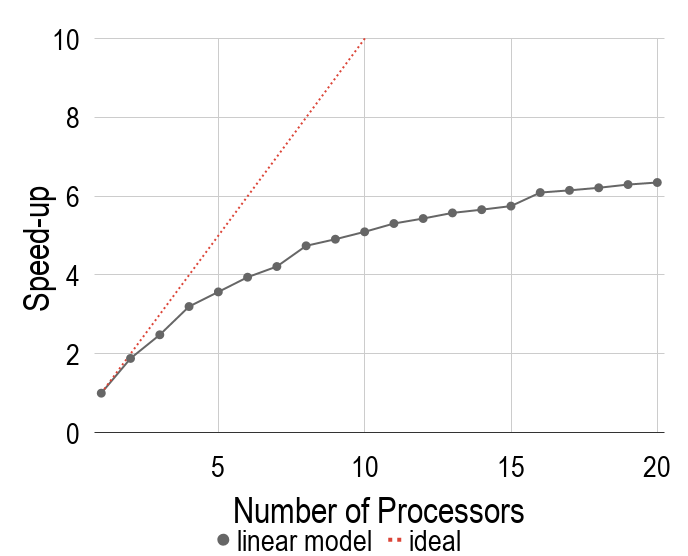
\includegraphics[width=0.45\textwidth]{figures/chapter-2/mm-parallel-model-tree-1-speedup.png}} &
		\subfloat[Theoretical speed-up of Model 2]{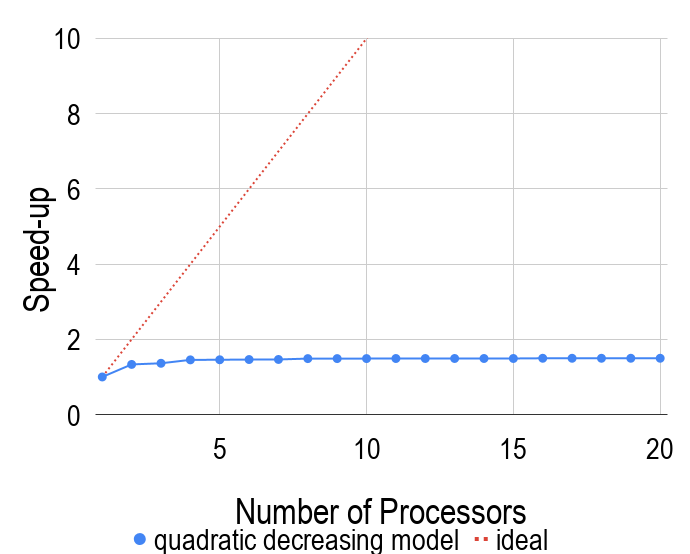
\includegraphics[width=0.45\textwidth]{figures/chapter-2/mm-parallel-model-tree-2-speedup.png}} \\
	\end{tabular}
	\caption{Theoretical speed-up}
	\label{fig:mm-parallel-model-speed-up}
\end{figure}


\begin{table}[htpb]
\centering
\begin{tabular}{|c|c|c|}
\hline
        & 20 PEs  & 32768 PEs \\ \hline
Model 1 & 6.3492  & 8.0000    \\ \hline
Model 2 & 1.4972 & 1.5000   \\ \hline
\end{tabular}
\caption{Potential speed-up of linear and quadratic models}
\label{table:mm-potential-model-speed-up}
\end{table}


We can see that model 1 still has some potential to grow whereas the second model has already reached its asymptote and further increase of processing elements does not make sense. In spite of a potential growth of the first model, both models have very low parallel efficiency even with 20 processing elements which can be observed from table \ref{table:mm-model-efficiency-20-pe}.\\


\begin{table}[htpb]
\centering
\begin{tabular}{|c|c|}
\hline
        & 20 PEs \\ \hline
Model 1 & 0.3175 \\ \hline
Model 2 & 0.0749 \\ \hline
\end{tabular}
\caption{Efficiency of linear and quadratic models using 20 PEs}
\label{table:mm-model-efficiency-20-pe}
\end{table}


Both models shows that computational intensity per node grows from bottom to top. It is easy to conclude from Figure \ref{fig:mm-parallel-model-tree} that intensity per node is equal $t/2^{i}$ and $t/2^{2i}$ for the first and second models, respectively (where $i$ is a level of the tree). It reflects that the most intensive part of the method is centered on the top part of the tree i.e. first few level. \citeauthor{mult-frontal-original:2} discussed application of the multifrontal method to a $k-by-k$ regular model problem with nine-point difference operator in his paper \cite{mult-frontal-original:2}. He observed that factorization of the last 6 nodes took slightly more than 25\% of the total amount of arithmetical operations. As a comparison, table \ref{table:mm-simple-model-work-load} shows fractions of time spent on processing first few top levels of our models: 1 and 2.\\


\begin{table}[htpb]
\centering
\begin{tabular}{|c|c|c|}
\hline
        & Model 1 & Model 2 \\ \hline
Level 0 & 6.25\%  & 50.00\% \\ \hline
Level 1 & 12.50\% & 75.00\% \\ \hline
Level 2 & 18.75\% & 87.50\% \\ \hline

\end{tabular}
\caption{Distribution workload per level in case model 1 and 2}
\label{table:mm-simple-model-work-load}
\end{table}


As we can see, the result of our first model is relatively close to 25\% and, therefore, it looks quite optimistic. However, the second model shows that 87\% of workload is focused on the top part of the tree and, as a result, we can consider that model as extremely pessimistic. \\


By and large, reduction of time spent on the top nodes is a way to improve strong scaling behavior. To do so, data parallelism can be additionally exploited for these nodes. It is worth noting that data parallelism at bottom levels does not make sense because it leads to increase of granularity there and thus increase communication overheads which can lead to significant performance drop.\\


Figure \ref{fig:mumps-task-data-parallelism} shows an example of two types of parallelism applied to the algorithm. First of all, we can see the leaves are grouped in subtrees and a single PE is assigned to each subtree. Other nodes are distributed among three different types. Nodes of the first type uses task parallelism only, which is induced by the tree, and each node is executed in a single processor. The second type exploits data parallelism with 1D block row distribution among the processors. The root belongs to the third type where data parallelism is used with 2D block cyclic distribution. The details of MUMPS parallelism management is carefully explained and can be found in \cite{mumps:task-data-parallelism}.\\


\figpointer{\ref{fig:mumps-task-data-parallelism}}

\begin{figure}[htpb]
  \centering
  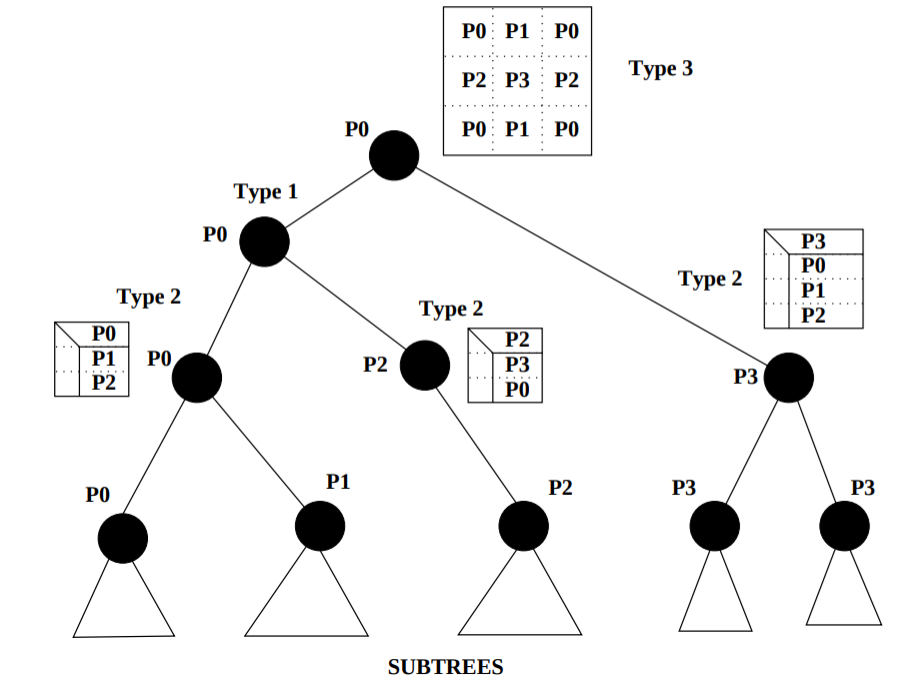
\includegraphics[width=0.65\textwidth]{figures/chapter-2/mumps-task-data-parallelism.png}
\caption{MUMPS parallelism management in case of 4 PEs \cite{mumps:task-data-parallelism}}
\label{fig:mumps-task-data-parallelism}
\end{figure}


All the techniques mentioned above were designed to improve strong scaling behavior by splitting the most intensive parts among all available processors. Going back to our models, we can also think about that in a slightly different way, namely: \textit{data parallelism helps to re-distribute cost per node/level on the corresponding elimination tree}. However, we have to notice that efficiency of data parallelism totally depends on sizes of frontal matrices at the top part of the tree. In case of skinny sparse matrices, oversubscription of processing elements can lead to strong performance penalties as we could see from section \ref{subseq:direct methods}. A machine-dependent minimal frontal matrix size was introduced in MUMPS in order to control whether to use ScaLAPACK at the root node or not \cite{mumps-manual}. It can happen that the algorithm uses only task parallelism, due to the threshold, and, as a results, scaling will only depend on the tree structure that can be deep and unbalanced.\\


Figure \ref{fig:model-1-vs-mumps} shows comparison of strong scaling between model 1 and parallel numerical factorization of the matrix \textit{\textbf{memchip}} (Table \ref{table:suite-sparse-matrix-set}) done with using MUMPS library. The sparsity pattern before and after fill-in reduction is shown in figure \ref{fig:memchip-matrix-sparsity-pattern}. 

\todo{add some examples to the appendix}
\figpointer{\ref{fig:model-1-vs-mumps}. Show standard deviation}
\begin{figure}[htpb]
  \centering
  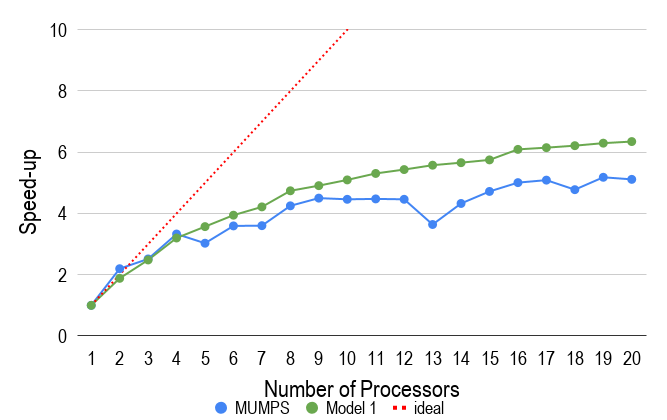
\includegraphics[width=0.65\textwidth]{figures/chapter-2/model-1-vs-mumps.png}
\caption{Comparison between model 1 and numerical factorization of the matrix \textit{\textbf{memchip}} using MUMPS library}
\label{fig:model-1-vs-mumps}
\end{figure}


\figpointer{\ref{fig:memchip-matrix-sparsity-pattern}}
\begin{figure}[htpb]
  \centering
  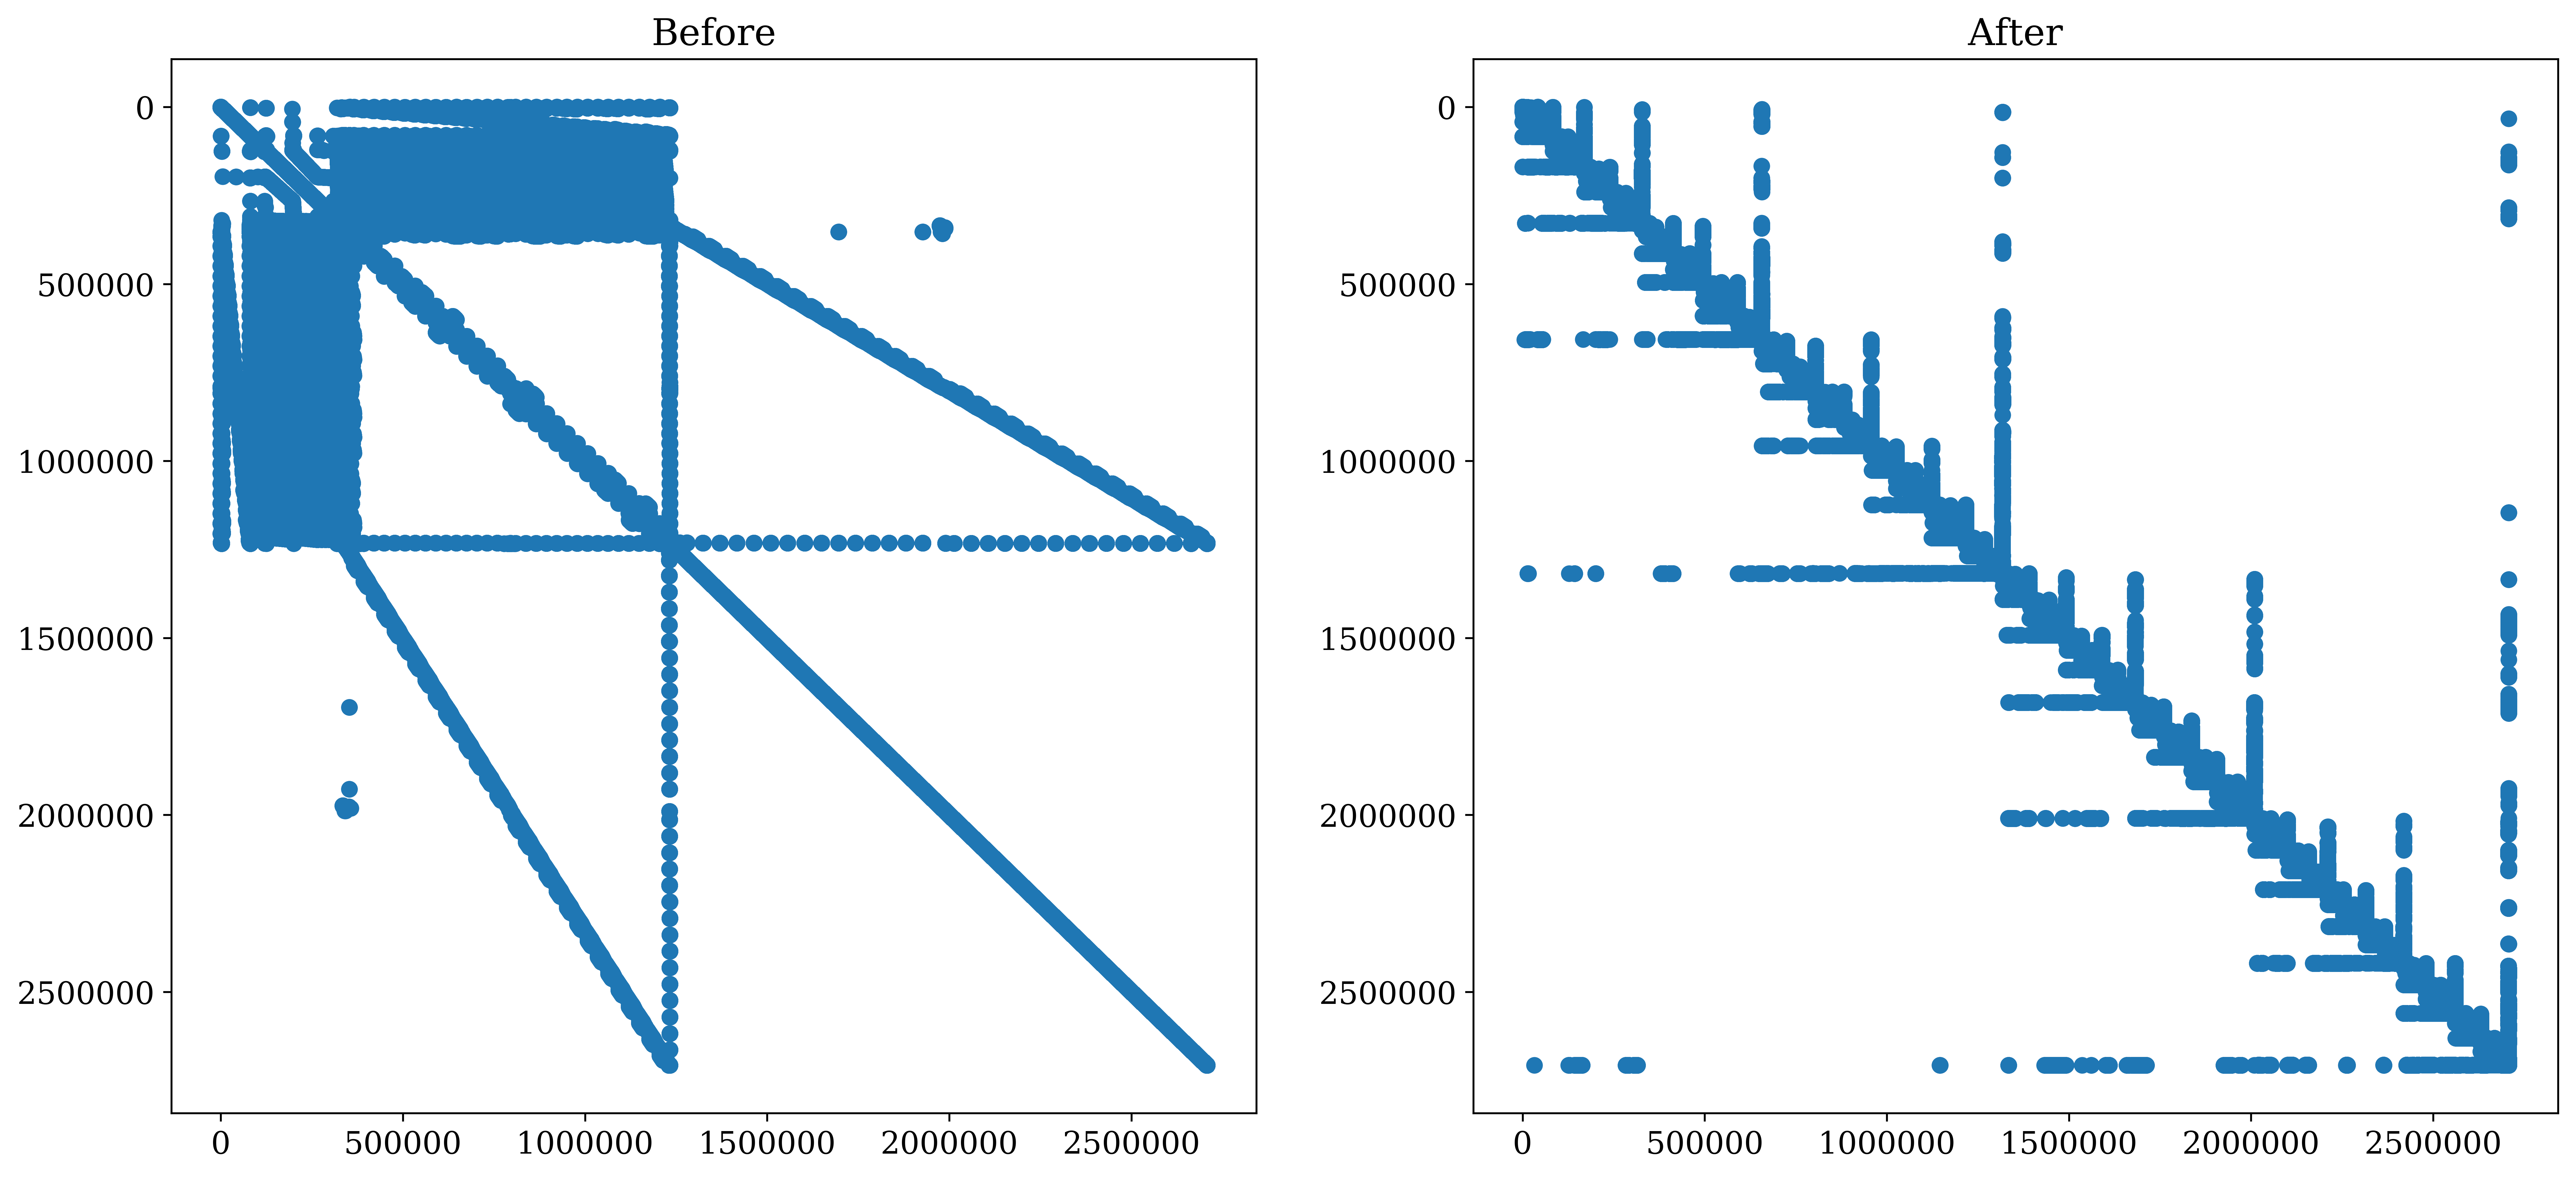
\includegraphics[width=1.00\textwidth]{figures/chapter-2/memchip-matrix-sparsity-pattern.png}
\caption{Sparsity structure of the matrix \textit{\textbf{memchip}} before and after fill-in reduction}
\label{fig:memchip-matrix-sparsity-pattern}
\end{figure}




As we can see, our model and the experiment show the same trend and the results are pretty much close to each other. However, our model takes into consideration only task parallelism whereas MUMPS exploits both data and task parallelism. Additionally, we have to mention that our model 1 works well only for relatively big sparse matrices. It can be quite inaccurate in case of small/skinny sparse systems. \\


In general, it is possible to refine our models and make them more accurate, using Bulk Synchronous Parallel (BSP) approach, for example. However, it will require to possess a real postordered elimination tree, extracted from a specific implementation of multifrontal method, together with information about supernodes sizes. We strongly believe the new enhanced model can explain the jagged strong scaling behavior of the MUMPS solver that we can observe in figure \ref{fig:model-1-vs-mumps}. But, this approach seems to be quite cumbersome and requires to delve into the source code of a particular library. It is needless to say that data can be retrieved only during run time and only after the analysis phase. This makes it less valuable and we can see that it is definitely a wrong way to go.\\


There are few important aspects to discuss at the end of the section. Numerical robustness is the main advantage of the multifrontal method. It does not require any preconditioner to solve a system of equations. As we discussed in the previous section, tuning a specific preconditioning algorithm can take a considerable amount of time, especially in case of our systems. As another advantage, the method (heavily) exploits matrix sparsity which lowers computational complexity up to $O(n^2)$. In case of massively huge matrices, the algorithm can utilize the secondary memory which sometimes is only one way to solve a system.\\


We can conclude, from the analysis above, the method has inherently bad scaling behavior and it is quite sensitive to a matrix structure. We will see later that it is almost impossible to predict the saturation point i.e. a point after which performance either drops or stays at the same level. We assume that scaling becomes better with growth of a matrix size. However, we cannot expect such behavior for small and medium systems.\\  


Secondly, we can see the algorithm requires many pre-processing steps to be done before numerical factorization phase. All these steps must run in parallel and be highly scalable. Apart from performance constrains of the steps, they must lead to wide and well balanced elimination trees which becomes crucial during the numerical phase.\\


Lastly, the algorithm can fail due to incorrect  working space prediction. As a results, factorization has to be restarted with some modification of input solver parameters.\\



\subsection{Results and Conclusion}
\label{subseq:hybrid-method-description}

Nowadays, iterative methods is a common choice for solving sparse systems of linear equations because of their possible fast convergence and high parallel efficiency. However, application of such method always demands preconditioning of ill-conditioned systems to make methods converge to numerical accurate solutions. It can be clearly observed from table \ref{table:grs-matrix-set} that numerical integration of thermo-hydraulic simulations in \gls{athlet} entails solving such ill-conditioned systems  based on estimated condition numbers of matrices form \gls{grs} matrix set.\\


As the first step of the study, we tested various preconditioning algorithms together with their tuning parameters, mentioned in table \ref{table:preconditioners}, applied to \gls{grs} matrix set. \gls{gmres} was chosen as an iterative solver with values of relative and absolute convergence tolerances in the residual norm to be equal to $1E-8$ and $1E-4$, respectively. A coarse grid search was used with maximum 3 values for each tuning parameter starting from the default towards more accurate values in order to refine settings of each preconditioning algorithm. Testing results showed that none of them could lead to convergence for the entire set of matrices.\\


One can assume that a finer grid search can result in finding a suitable preconditioning algorithm with settings that can lead to convergence of \gls{gmres} solver for the entire set. However, it is important to point out the matrices were generated by running the most common \gls{grs} thermo-hydraulic test-scenarios and saving them somewhere during the time integration process. Hence, there is no guarantee that the settings found in such a way can always lead to convergence of \gls{gmres} solver in all time steps of any thermo-hydraulic simulation. Therefore, iterative methods may not satisfy \textit{robustness} criteria stated in chapter \ref{chapter:problem-statment} as a non-functional requirement to the time integration solver used in \gls{athlet}.\\


Taking into account the above reasoning, we have come to the conclusion that sparse direct methods is the best choice for our problem, in spite of the limited tree-task parallelism described in subsection \ref{subseq:direct-parallel-aspects}, because the methods stably result in numerical accurate solutions even in case of ill-conditioned linear systems. Hence, the next objective of the study is to find a suitable sparse direct method and its implementation, and adapt it for \gls{hw1} compute-cluster environment in terms of efficient parallel execution. \\



	\section{Selection of a Sparse Direct Linear Solver} \label{chapter:solver-selection}
	\label{subseq:mm-library-choice}

Fair to say, there is no single algorithm or software that is the best for all types of linear systems \cite{list-of-sparse-direct-solvers}.\\


Nowadays, there exist many different avaliable sparse direct solvers. Some of them are tunned for specific linear systems whereas others are targeted for the most general cases \cite{list-of-sparse-direct-solvers}. Some of them handle tree-task and node-data parallelism in different ways even within the same library depending on sizes of frontal matrices and other criteria \cite{wsmp}, \cite{mumps-manual}, \cite{superlu-manual}. Hence, parallel performance of a direct sparse method depends heavily on its specific implementation. Table \ref{table:mm-library-spec} represents a short summary of almost all available libraries capable to run on distributed-memory machines, at the time of writing, based on works \cite{list-of-sparse-direct-solvers} and \cite{petsc-web-page}.\\


\begin{table}[ht]
\small
\centering
\begin{tabular}{|c|c|c|c|c|}
\hline
Package & Method             & Matrix Types                 & \multicolumn{1}{c|}{\begin{tabular}[c]{@{}c@{}}PETSc\\ Interface\end{tabular}} & License      \\ \hline
Clique       & Multifrontal       & Symmetric      & \multicolumn{1}{c|}{\begin{tabular}[c]{@{}c@{}}Not \\ Officially\end{tabular}} & Open  \\ \hline
MF2          & Multifrontal       & \begin{tabular}[c]{@{}c@{}}Symmetric\\ pattern\end{tabular} & No              & -            \\ \hline
DSCPACK      & Multifrontal       & SPD                          & No              & Open* \\ \hline
MUMPS        & Multifrontal       & General                      & Yes             & Open  \\ \hline
PaStiX       & Left looking & General                      & Yes             & Open  \\ \hline
PSPASES      & Multifrontal       & SPD                          & No              & Open* \\ \hline
SPOOLES      & Left-looking       & \begin{tabular}[c]{@{}c@{}}Symmetric\\ pattern\end{tabular} & No              & Open* \\ \hline
SuperLU\_DIST & Right-looking      & General                      & Yes             & Open  \\ \hline
symPACK      & Left-Right looking & SPD                          & No              & Open  \\ \hline
S+           & Right-lookin       & General                      & No              & -            \\ \hline

PARDISO         & Multifrontal       & General                      & No              & Commercial   \\ \hline

WSMP         & Multifrontal       & General                      & No              & Commercial   \\ \hline
\end{tabular}
\caption{A list of direct sparse linear solvers adapted for distributed-memory computations, \cite{list-of-sparse-direct-solvers}, \cite{petsc-web-page}.\\}
where SPD - Symmetric Positive Definite; 
Open* - an interface is not officially supported by the \acrshort{petsc} team
\label{table:mm-library-spec}
\end{table}


It can be clearly observed, from Table \ref{table:mm-library-spec}, that only \acrshort{mumps}, PaStiX and SuperLU\_DIST cover all requirements induced by \acrshort{grs}, see Chapter \ref{chapter:problem-statment}, in particular: open-source license and a direct interface to \acrshort{petsc}. It is interesting to notice that all libraries, mentioned above, are implementations of different sparse direct methods, namely: multi-frontal (\acrshort{mumps}), left-looking (PaStiX) and right-locking (SuperLU\_DIST). Moreover, PaStiX and SuperLU\_DIST use only static pivoting \cite{pastix-manual}, \cite{superlu-manual} whereas \acrshort{mumps} provides a full implementation of the threshold pivoting strategy \cite{mumps-manual}, described in Subsection \ref{subseq:pivot-hadling}.\\


To compare the libraries, a couple of flat-\acrshort{mpi} tests were performed using \acrshort{grs} matrix set on \gls{hw1} machine. \acrshort{petsc} library was compiled and configured with \acrshort{mumps} (version 5.1.2), PasTiX (version 6.0.0) and SuperLU\_DIST (version 5.4) packages using their default parameter settings. An internal built-in \acrshort{petsc} profiler was used to measure execution time.  A time limit of 15 minutes was set up for each test-case to prevent blocking of a cluster compute-node from an unexpected long program execution. Results are summarized in Tables \ref{table:lc-cube-5-result}, \ref{table:lc-cube-64-result}, \ref{table:lc-k3-18-result} and in appendix \ref{app:app-lc} where numerical values are given in seconds.\\



\begin{table}[ht]
\centering
\begin{tabular}{|c|c|c|c|l|c|c|c|c|}
\cline{1-4} \cline{6-9}
MPI & MUMPS    & PaStiX   & SuperLU  &  & MPI & MUMPS    & PaStiX   & SuperLU  \\ \cline{1-4} \cline{6-9} 
1   & 7.02E-02 & 8.72E-02 & 3.17E+00 &  & 11  & 7.55E-02 & 8.89E-02 & 5.82E-01 \\ \cline{1-4} \cline{6-9} 
2   & 6.73E-02 & 7.10E-02 & 1.43E+00 &  & 12  & 7.61E-02 & 1.06E-01 & 4.37E-01 \\ \cline{1-4} \cline{6-9} 
3   & 6.36E-02 & 7.01E-02 & 1.07E+00 &  & 13  & 7.84E-02 & 9.72E-02 & 5.43E-01 \\ \cline{1-4} \cline{6-9} 
4   & 6.28E-02 & 7.11E-02 & 8.17E-01 &  & 14  & 8.06E-02 & 1.02E-01 & 4.22E-01 \\ \cline{1-4} \cline{6-9} 
5   & 6.50E-02 & 7.15E-02 & 7.51E-01 &  & 15  & 8.20E-02 & 1.19E-01 & 3.91E-01 \\ \cline{1-4} \cline{6-9} 
6   & 6.72E-02 & 7.62E-02 & 6.15E-01 &  & 16  & 8.07E-02 & 1.19E-01 & 4.44E-01 \\ \cline{1-4} \cline{6-9} 
7   & 6.91E-02 & 7.69E-02 & 6.48E-01 &  & 17  & 8.38E-02 & 1.22E-01 & 5.19E-01 \\ \cline{1-4} \cline{6-9} 
8   & 6.89E-02 & 8.17E-02 & 5.41E-01 &  & 18  & 8.40E-02 & 1.26E-01 & 3.77E-01 \\ \cline{1-4} \cline{6-9} 
9   & 7.50E-02 & 8.28E-02 & 5.02E-01 &  & 19  & 8.58E-02 & 1.33E-01 & 5.47E-01 \\ \cline{1-4} \cline{6-9} 
10  & 7.22E-02 & 8.52E-02 & 4.64E-01 &  & 20  & 8.64E-02 & 1.49E-01 & 3.39E-01 \\ \cline{1-4} \cline{6-9} 
\end{tabular}
\caption{Comparisons of parallel performance of  \textit{cube-5} matrix factorization using \acrshort{mumps}, PasTiX and SuperLU\_DIST solvers with their default parameter settings}
\label{table:lc-cube-5-result}
\end{table}


\begin{table}[ht]
\centering
\begin{tabular}{|c|c|c|c|l|c|c|c|c|}
\cline{1-4} \cline{6-9}
MPI & MUMPS    & PaStiX   & SuperLU  &  & MPI & MUMPS    & PaStiX   & SuperLU  \\ \cline{1-4} \cline{6-9} 
1   & 1.36E+00 & 1.39E+00 & time-out &  & 11  & 7.75E-01 & 8.15E-01 & time-out \\ \cline{1-4} \cline{6-9} 
2   & 1.00E+00 & 9.82E-01 & time-out &  & 12  & 7.81E-01 & 8.10E-01 & time-out \\ \cline{1-4} \cline{6-9} 
3   & 8.83E-01 & 1.06E+00 & time-out &  & 13  & 7.85E-01 & 8.35E-01 & time-out \\ \cline{1-4} \cline{6-9} 
4   & 8.17E-01 & 8.74E-01 & time-out &  & 14  & 7.85E-01 & 8.18E-01 & time-out \\ \cline{1-4} \cline{6-9} 
5   & 7.85E-01 & 8.50E-01 & time-out &  & 15  & 7.88E-01 & 8.46E-01 & time-out \\ \cline{1-4} \cline{6-9} 
6   & 8.06E-01 & 8.52E-01 & time-out &  & 16  & 7.81E-01 & 8.23E-01 & time-out \\ \cline{1-4} \cline{6-9} 
7   & 7.71E-01 & 8.33E-01 & time-out &  & 17  & 6.83E-01 & 8.49E-01 & time-out \\ \cline{1-4} \cline{6-9} 
8   & 7.66E-01 & 8.33E-01 & time-out &  & 18  & 7.96E-01 & 8.44E-01 & time-out \\ \cline{1-4} \cline{6-9} 
9   & 7.93E-01 & 8.35E-01 & time-out &  & 19  & 8.04E-01 & 8.65E-01 & time-out \\ \cline{1-4} \cline{6-9} 
10  & 8.07E-01 & 8.15E-01 & time-out &  & 20  & 6.85E-01 & 8.87E-01 & time-out \\ \cline{1-4} \cline{6-9} 
\end{tabular}
\caption{Comparisons of parallel performance of  \textit{cube-64} matrix factorization using \acrshort{mumps}, PasTiX and SuperLU\_DIST solvers with their default parameter settings}
\label{table:lc-cube-64-result}
\end{table}


\begin{table}[h!]
\centering
\begin{tabular}{|c|c|c|c|l|c|c|c|c|}
\cline{1-4} \cline{6-9}
MPI & MUMPS    & PaStiX   & SuperLU &  & MPI & MUMPS    & PaStiX   & SuperLU \\ \cline{1-4} \cline{6-9} 
1   & 1.55E+02 & 6.44E+01 & crashed &  & 11  & 1.77E+01 & 3.81E+01 & crashed \\ \cline{1-4} \cline{6-9} 
2   & 6.28E+01 & 4.84E+01 & crashed &  & 12  & 1.60E+01 & 3.75E+01 & crashed \\ \cline{1-4} \cline{6-9} 
3   & 5.06E+01 & 5.02E+01 & crashed &  & 13  & 1.42E+01 & 3.58E+01 & crashed \\ \cline{1-4} \cline{6-9} 
4   & 4.17E+01 & 4.50E+01 & crashed &  & 14  & 1.45E+01 & 3.59E+01 & crashed \\ \cline{1-4} \cline{6-9} 
5   & 2.52E+01 & 3.98E+01 & crashed &  & 15  & 1.47E+01 & 3.57E+01 & crashed \\ \cline{1-4} \cline{6-9} 
6   & 2.58E+01 & 4.29E+01 & crashed &  & 16  & 1.41E+01 & 3.52E+01 & crashed \\ \cline{1-4} \cline{6-9} 
7   & 2.65E+01 & 4.30E+01 & crashed &  & 17  & 1.54E+01 & 3.45E+01 & crashed \\ \cline{1-4} \cline{6-9} 
8   & 2.59E+01 & 3.73E+01 & crashed &  & 18  & 1.52E+01 & 3.31E+01 & crashed \\ \cline{1-4} \cline{6-9} 
9   & 1.95E+01 & 4.08E+01 & crashed &  & 19  & 1.52E+01 & 3.31E+01 & crashed \\ \cline{1-4} \cline{6-9} 
10  & 1.91E+01 & 3.81E+01 & crashed &  & 20  & 1.38E+01 & 3.16E+01 & crashed \\ \cline{1-4} \cline{6-9} 
\end{tabular}
\caption{Comparisons of parallel performance of \textit{k3-18} matrix factorization using \acrshort{mumps}, PasTiX and SuperLU\_DIST solvers with their default parameter settings}
\label{table:lc-k3-18-result}
\end{table}



Some problems were detected during  SuperLU\_DIST library testing. First of all, executions of \textit{cube-64} and \textit{k3-2} test-cases exceeded the set time limit. Secondly, it was noticed the library was crashing during processing of \textit{k3-18}, \textit{cube-645} and (partially) \textit{pwr-3d} test-cases. Debugging revealed that a segmentation fault occurred in function \textit{pdgstrf}  during the numerical factorization phase. Nonetheless, it is still unclear whether the problem was software or hardware specific. A solution or a reason of such program behavior has not been found at the moment of writing.\\


% FOR PRESENTATION: it can be due to wrong matrix representation in binary \acrshort{petsc} files. I ran into the same problem with METIS when it spinned the CPU for hours due to wrong CRS format

To complete comparison and evaluate parallel performance SuperLU\_DIST library, an additional test was conducted using a 2D formulation of the Poisson problem with \textit{100000} unknown. According to the results, SuperLU\_DIST managed to complete matrix factorizations within the set time limit without crashing, however, it showed abnormal jagged strong scaling behavior. Moreover, it turned out it was the slowest in comparison to the other solvers. The results are shown in Figure \ref{fig:5-point-stencil-solvers-comparison}.\\



\figpointer{\ref{fig:5-point-stencil-solvers-comparison}}
\begin{figure}[htpb]
  \centering
  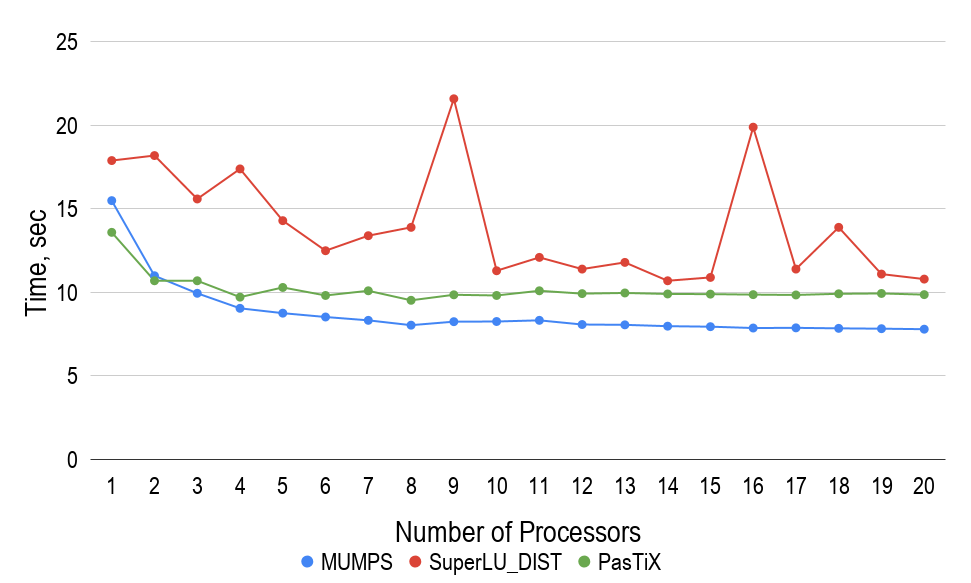
\includegraphics[width=0.85\textwidth]{figures/chapter-2/solvers-comparison-5-point-stencil.png}
\caption{Comparisons of parallel performance of 5 point-stencil Poisson matrix (1000000  equations) factorization using 
\acrshort{mumps}, PasTiX and SuperLU\_DIST libraries with their default parameter settings}
\label{fig:5-point-stencil-solvers-comparison}
\end{figure}

% FOR PRESENTATION: we think that 

According to the initial and additional tests, \acrshort{mumps} library showed the best parallel performance and scaling in contrast to the other solvers. No abnormal behavior during its operation was detected. In some cases, it only required to increase a multiplicative factor of estimated working space which was used to hold frontal matrices and factors $L$ and $U$ in memory. PaStiX was the second fastest solver according to the results of testing. However,  it was often considerably slower than \acrshort{mumps}. At the same time, SuperLU\_DIST showed the worst results. Additionally, as it was mentioned above, we experienced some technical problems during operation of this library.\\


A literature review showed quite contradictory results and conclusions. For example, \citeauthor{wsmp}, in work \cite{wsmp}, came to nearly the same outcome, as we did, comparing parallel performance of WSMP, \acrshort{mumps} and SuperLU\_DIST libraries using their matrix set. However, \citeauthor{mm-comparison-of-packages} showed, in \cite{mm-comparison-of-packages}, that SuperLU\_DIST spent the least amount of time on solving  systems of linear equations in contrast to the other solvers used in their work. It needless to say that both research groups used different matrix sets and hardware. Nevertheless, it reveals a quite important fact that a selection of a particular method and its implementation can depend heavily on a specific matrix set.\\


In this section, we compared different sparse direct methods and their concrete implementations using their default parameter settings with regard to \acrshort{grs} matrix set. Based on the obtained results and literature review, \acrshort{mumps} library was chosen for the following study. In Section \ref{subseq:mumps-review}, we make an overview of the library and its specific traits. \\


	\section{Overview of \acrshort{mumps} Library}
	\subsection{Review of MUMPS Library}
\label{subseq:mumps-review}

\todo{read comments}
%All the techniques mentioned above were designed to improve strong scaling behavior by splitting the most intensive parts among all available processors. Going back to our models, we can also think about that in a slightly different way, namely: \textit{data parallelism helps to re-distribute cost per node/level on the corresponding elimination tree}. However, we have to notice that efficiency of data parallelism totally depends on sizes of frontal matrices at the top part of the tree. In case of skinny sparse matrices, oversubscription of processing elements can lead to strong performance penalties as we could see from section \ref{subseq:direct methods}. A machine-dependent minimal frontal matrix size was introduced in MUMPS in order to control whether to use ScaLAPACK at the root node or not \cite{mumps-manual}. It can happen that the algorithm uses only task parallelism, due to the threshold, and, as a results, scaling will only depend on the tree structure that can be deep and unbalanced.\\



Originally, MUltifrontal Massively Parallel sparse direct Solver (MUMPS) was a part of the PARASOL Project. The project was an ESPRIT IV long term research with the main goal to build and test a portable library for solving large sparse systems of equations on distributed memory systems \cite{PARASOL}. An important aspect of the researh was a strong link between the developers of the sparse solvers and industrial end users, who provided a range of test problems and evaluated the solvers \cite{MUMPS:description}. Since 2000 MUMPS had continued as an ongoing project and, by the time of writing, the library have contained almost 5 main releases.\\



As it was mentioned in section \ref{subseq:mm-library-choice}, MUMPS is an implementation of the multi-frontal method. Therefore, MUMPS performs all three phases in sequence, namely: analysis, numerical factorization and solution. The numerical factorization and solution phases were fully described in detail in subsection \ref{subseq:direct-sparse methods}. In this subsection, the analysis phase of MUMPS is examined since implementation of this phase often varies between libraries due to different parallel performance considerations.\\


According to the library documentation, the analysis phases of MUMPS consists of several pre-processing steps:

\begin{enumerate}
  \item Fill-reducing pivot order \label{mumps:analysis-steps:1}
  \item Symbolic factorization \label{mumps:analysis-steps:2}
  \item Scaling \label{mumps:analysis-steps:3}
  \item Amalgamantion \label{mumps:analysis-steps:4}
  \item Mapping \label{mumps:analysis-steps:5}
\end{enumerate}


% Fill-reducing pivot order
\ref{mumps:analysis-steps:1}) To handle both symmetric and unsymmetric cases, MUMPS performs fill-reducing reordering based on $\boldsymbol{A} + \boldsymbol{A^T}$ sparsity pattern. The library provides numerous sequantial algorithms for the reordering such as Approximate Minimum Degree (AMD) \cite{reordering:AMD}, Approximate Minimum Fill (AMF), Approximate Minimum Degree with automatic quasi-dense row detection (QAMD) \cite{reordering:QAMD}, Bottom-up and Top-down Sparse Reordering (PORD) \cite{reordering:PORD}, Nested Dissection coupled with AMD (Scotch) \cite{reordering:SCOTCH}, Multilevel Nested Dissection coupled with Multiple Minimum Degree (METIS) \cite{reordering:METIS}. Additionally, MUMPS can work together with ParMETIS and PT-Scotch which are extensions of METIS and Scotch libraries for parallel execution, respectively. MUMPS also provides the user with an option to select a fill-in reducing algorithm in run-time based on matrix type, size and the number of processors \cite{mumps-manual}.\\


% Symbolic factorization
\ref{mumps:analysis-steps:2}) Sparsity structures of factors $L$ and $U$ are computed during the symbolic factorization pre-processing step, based on permuted matrix $A$ after fill-in reducing reordering. It gives the input information for elimination tree building process.  All computations at this step are performed using a directed graph $G(A)$ associated with the matrix $A$.\\


% Scaling
\ref{mumps:analysis-steps:3}) Matrix $A$ is tried to scale in such a way to get absolute values of \textit{one} along the main diagonal and \textit{less than one} for all off-diagonal entries. Scaling algorithms are described in detail in works \cite{mm:scaling:duff1999design}, \cite{mm:scaling:duff2001algorithms} (for the unsymmetric case) and \cite{mm:scaling:duff2005strategies} (for the symmetric case). This pre-processing step is supposed to improve numerical accuracy and makes all estimations performed during analysis more reliable \cite{mumps-manual}. MUMPS also provides an option to switch off scaling or perform it during the factorization phase.\\



% Amalgamantion
\ref{mumps:analysis-steps:4}) During amalgamation step, described in subsection \ref{subseq:direct-sparse methods}, sets of columns with the same off-diagonal sparsity pattern are group together to create denser nodes, also known as super-nodes. The process leads to restructuring of the initial elimination tree to an amalgamated one of super-nodes which is also know as the \textit{assembly tree}. The main purpose of this step is to improve efficiency of dense matrix operations.\\



% Mapping
\ref{mumps:analysis-steps:5}) A host process, chosen by MUMPS, creates a pool of tasks where each task belongs to one out of three different types, figure \ref{fig:mumps:mapping-and-scheduling}. Then, the host distributes tasks among all available processes in such a way to achieve good memory and compute balance.\\

 
Type 1 nodes are grouped in subtrees, according to the Geist-Ng algorithm \cite{geist1989task}, and each subtree is processed by a single process to avoid the finest granularity, which can cause high communication overheads. \\


In case of type 2 nodes, the host process assigns each node to one process, called the \textit{master}, which holds fully summed rows and columns of a node as well as performs pivoting and partial factorization. During the numerical factorization phase, in run-time, a master process first receives symbolic information, describing  contribution block structures, from its children. Then, the master collects information concerning the load balance of all other processes and decides, \underline{\textit{dynamically}},  which of them, \textit{slaves}, are going to participate to the node factorization. After that, the master informs the chosen slaves that a new task has been allocated for them, maps them according to 1D block column distribution and sends them the corresponding parts of the frontal matrix. Then, the slaves communicate the children of the master process and collect the corresponding numerical values. The slaves are in charge of assembly and computations of the partly summed rows. The computational process is illustrated in figure \ref{fig:mumps:steps-of-type-2-factorization}, subsection \ref{subseq:blas-comparison}.\\


The root node belongs to the type 3. The host \underline{\textit{statically}} assigns the master for the root, as it is in case of type 2 nodes, to hold all the indices describing the structure of its frontal matrix. Before factorization, the structure of the root frontal matrix is statically mapped onto a 2D grid of processes using block cyclic distribution. This allows to determine, during the analysis phase, which process an entry of the root is assigned. Hence, the original matrix entries and the part of the contribution blocks can be assembled as soon as they are available. Because of threshold pivoting, the master process collects the information of indices for all delayed variables of its sons, builds the final structure of the root frontal matrix and broadcast the corresponding symbolic information to all slaves. The slaves, in turn, adjust their local data structure and, right after that, perform numerical factorization in parallel.\\


It is important to mention if the root node size is less than a certain computer depended parameter, defined internally by MUMPS, the root node will be treated as the type 2, \cite{mumps-manual}.\\


An example of static/dynamic scheduling i.e. process mapping, is represented in figure \ref{fig:mumps:mapping-and-scheduling}.\\


\figpointer{\ref{fig:mumps:mapping-and-scheduling}}
\begin{figure}[htpb]
  \centering
  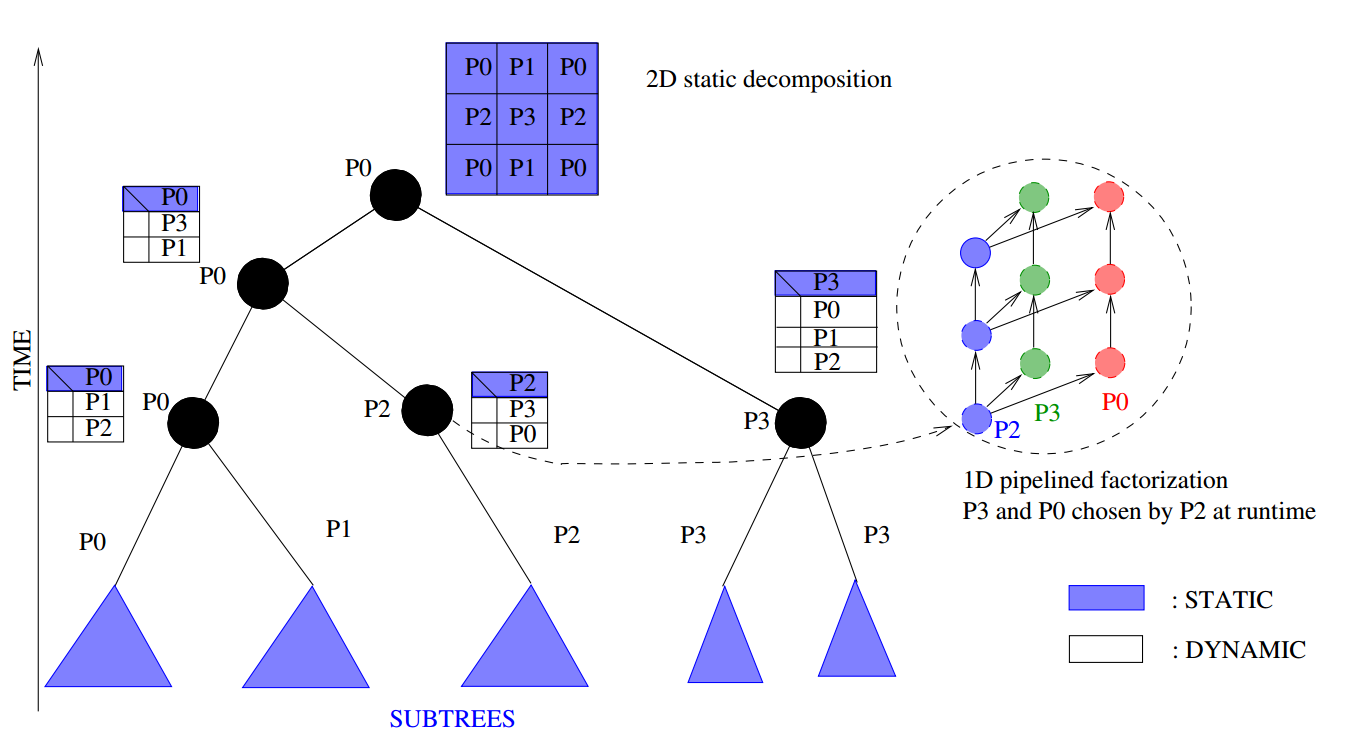
\includegraphics[width=0.85\textwidth]{figures/chapter-2/mumps-task-data-parallelism-2.png}
\caption{MUMPS: static and dynamic scheduling \cite{l2012multifrontal}}
\label{fig:mumps:mapping-and-scheduling}
\end{figure}







	\section{Configuration of MUMPS Library} 
	\label{mumps:solver-configuration}
	
	This section is organized as follows. Each subsection describes configuration of \acrshort{mumps} with particular techniques, methods or libraries stated in the title of a subsection, \textit{e.g. Subsection \ref{subseq:blas-comparison}, i.e. 
"Optimized \acrshort{blas} Implementations", stands for 
"Configuration of MUMPS Library with Optimized \acrshort{blas} Implementations"}.\\	
	
	
	
\section{Choice of Fill Reducing Reordering}
\label{subseq:fill-in-reordering}

Fill reducing reordering is the first and the most important step since it has its direct impact on the assembly tree structure. As we mentioned above, the tree structure defines the task parallelism as well as sizes of frontal matrices and thus performance of the method.\\

MUMPS provides various algorithms for reordering described in section \ref{subseq:mumps-review}. A detailed study and comparison between different methods were done by \citeauthor{guermouche2003memory} in work \cite{guermouche2003memory} in case of sequential execution of the analysis phase. \citeauthor{guermouche2003memory} noticed that the trees generated by METIS and SCOTCH were rather wide (because of the global partitioning performed at the top), while the trees generated by AMD, AMF and PORD tend to be deeper. In addition, they came to two important conclusions. Firstly, they noticed both SCOTCH and METIS generated much better balanced trees in contrast to other methods. Secondly, according to their results, SCOTCH and METIS generated trees with frontal matrices bigger than those generated by the other reorderings \cite{guermouche2003memory}.\\


In this section we are going to investigate parallel performance of PT-Scotch and ParMETIS packages as well as MUMPS automatic run-time library selection in case of GRS matrix set. The algorithmic difference between PT-Scotch and ParMETIS was explained in section \ref{subseq:mumps-review}.\\


To perform a test, the default PETSc, MUMPS, PT-Scotch and ParMETIS libraries were downloaded, compiled and configured together. The test was carried out using only flat-MPI mode without explicit process pinning. The results are shown in figure BRA and in appendix BRA-BRA.\\


\figpointer{\ref{fig:mumps-ordering-1}}
\begin{figure}[htpb]
\centering
	\begin{tabular}{cc}
		\subfloat[k3-18]{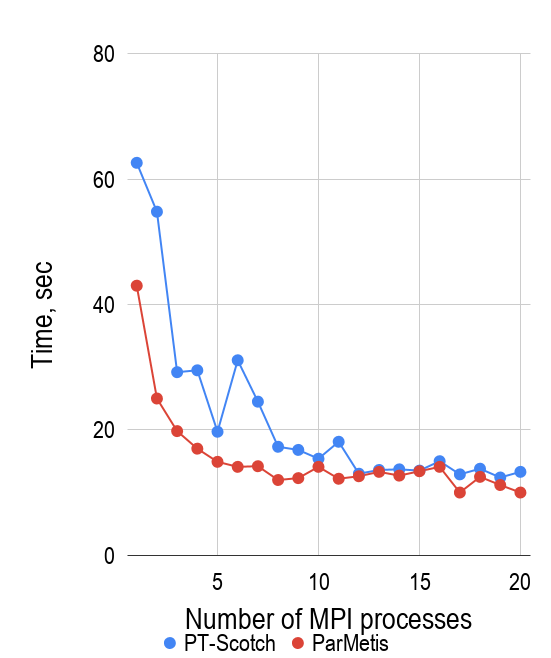
\includegraphics[width=0.48\textwidth]{figures/chapter-2/ordering/k3-18.png}} &
		\subfloat[cube-64]{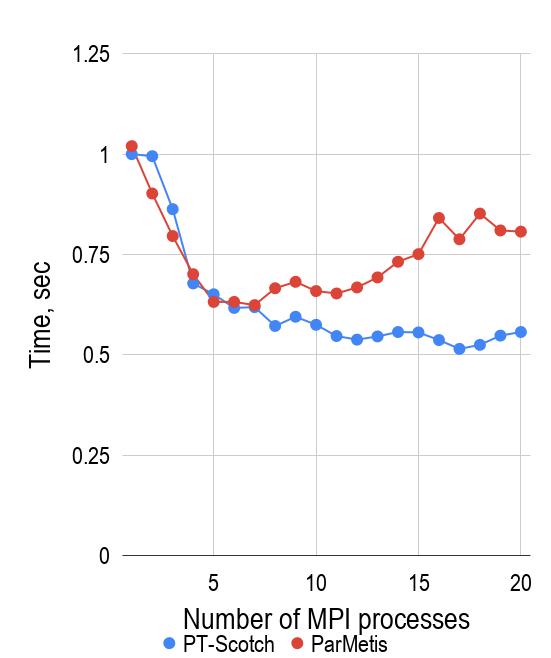
\includegraphics[width=0.48\textwidth]{figures/chapter-2/ordering/cube-64.png}} \\
		\subfloat[pwr-3d]{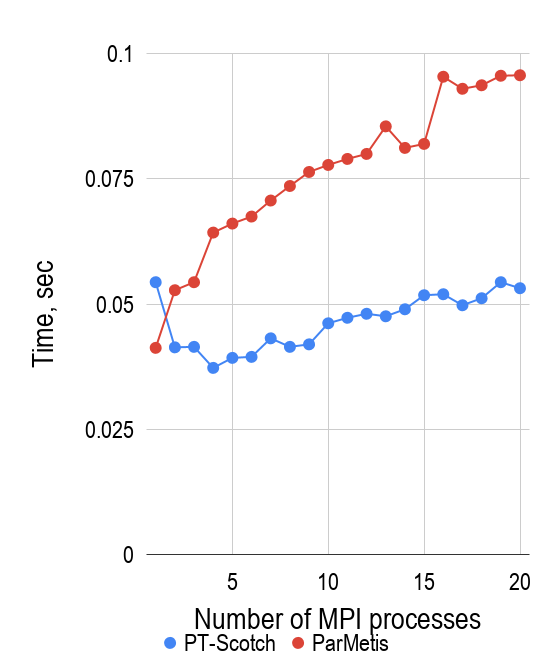
\includegraphics[width=0.48\textwidth]{figures/chapter-2/ordering/pwr-3d.png}} &
		\subfloat[k3-2]{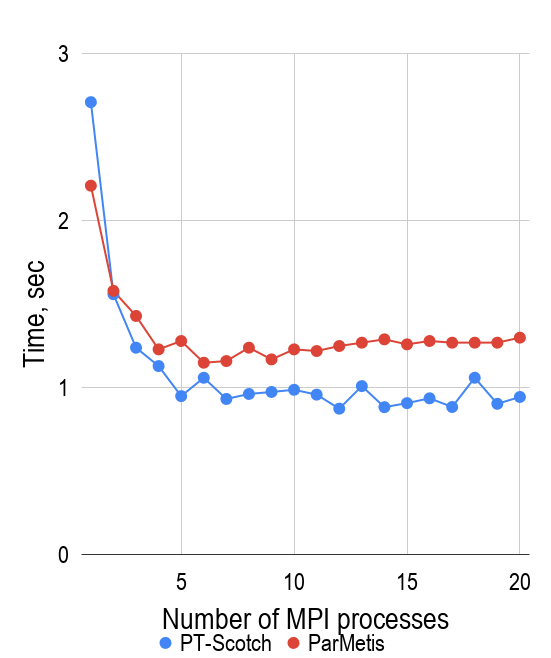
\includegraphics[width=0.48\textwidth]{figures/chapter-2/ordering/k3-2.png}} \\
	\end{tabular}
	\caption{Comparison of different fill-reducing algorithms}
	\label{fig:mumps-ordering-1}
\end{figure}



As the results show, ParMETIS scales much better in contrast to PT-Scotch. In average, the run-time is reduced by approximately BLA \% and BRA \% around the saturation point. Unfortunately, it is difficult for us to give a detailed explanation of the results because there is no access to the assembly tree structure from outside of MUMPS, known to us. Additionally, profiling and tracing of both packages, ParMETIS and PT-Scotch, are required which is out of the scope of this study.\\



\begin{table}[htpb]
\centering
\begin{tabular}{|c|c|c|c|c|}
\hline
Matrix Name & Ordering  & n       & nnz      & nnz / n \\ \hline
cube-5      & PT-Scotch & 9325    & 117897   & 12.6431 \\ \hline
cube-64     & PT-Scotch & 100657  & 1388993  & 13.7993 \\ \hline
cube-645    & ParMetis  & 1000045 & 13906057 & 13.9054 \\ \hline
k3-2        & PT-Scotch & 130101  & 787997   & 6.0568  \\ \hline
k3-18       & ParMetis  & 1155955 & 7204723  & 6.2327  \\ \hline
pwr-3d      & PT-Scotch & 6009    & 32537    & 5.4147  \\ \hline
\end{tabular}
\end{table}


\begin{table}[htpb]
\centering
\begin{tabular}{|c|c|c|c|c|}
\hline
Matrix Name & Ordering  & n       & nnz      & nnz / n \\ \hline
cant        & ParMetis  & 62451   & 4007383  & 64.1684 \\ \hline
consph      & PT-Scotch & 83334   & 6010480  & 72.1252 \\ \hline
memchip     & PT-Scotch & 2707524 & 13343948 & 4.9285  \\ \hline
PFlow\_742  & PT-Scotch & 742793  & 37138461 & 49.9984 \\ \hline
pkustk10    & PT-Scotch & 80676   & 4308984  & 53.4110 \\ \hline
torso3      & ParMetis  & 259156  & 4429042  & 17.0903 \\ \hline
x104        & PT-Scotch & 108384  & 8713602  & 80.3956 \\ \hline
CurlCurl\_3 & PT-Scotch & 1219574 & 13544618 & 11.1060 \\ \hline
Geo\_1438   & xxx       & 1437960 & 63156690 & 43.9210 \\ \hline
nlpkkt80    & xxx       & 1062400 & 28192672 & 26.5368 \\ \hline
\end{tabular}
\end{table}





\section{MUMPS: Process Pinning}
\label{subseq:mm-mumps-process-pinning}

Due to intensive and complex manipulations with frontal and and contribution matrices, we can assume that MUMPS belongs to memory bound applications. In this case memory access can be a bottleneck for the library. A common way to improve performance of memory bound applications running on distributed memory machines is to distribute processes equally among sockets of a node.\\


However, because MUMPS uses both task and data parallelism as well as a complex hybrid, both static and dynamic, task scheduling, it becomes difficult to decide which pinning strategy is better i.e. \textit{close} or \textit{spread}, described in section \ref{subseq:matrix-sets-and-hardware}.\\


Therefore, a couple of tests were conducted with both GRS and SuiteSparse matrix sets in order to investigate influence of different strategies on MUMPS performance. For this group of tests, only MUMPS default settings together with a specific fill-in reducing algorithm for each test case, mentioned in section \ref{subseq:fill-in-reordering}, were used. The tests were performed on HW1 machine using only flat-MPI mode. Results are shown in figures \ref{fig:mumps-close-vs-spread-1}, \ref{fig:mumps-close-vs-spread-2}, \ref{fig:mumps-close-vs-spread-3} and in appendix \ref{app:mm-mumps-process-pinning}. The graphs depict the total time spent, i.e. analysis, factorization and solution.\\

\figpointer{\ref{fig:mumps-close-vs-spread-1}}
\begin{figure}[htpb]
\centering
	\begin{tabular}{cc}
	\subfloat[HW1 - pwr-3d]{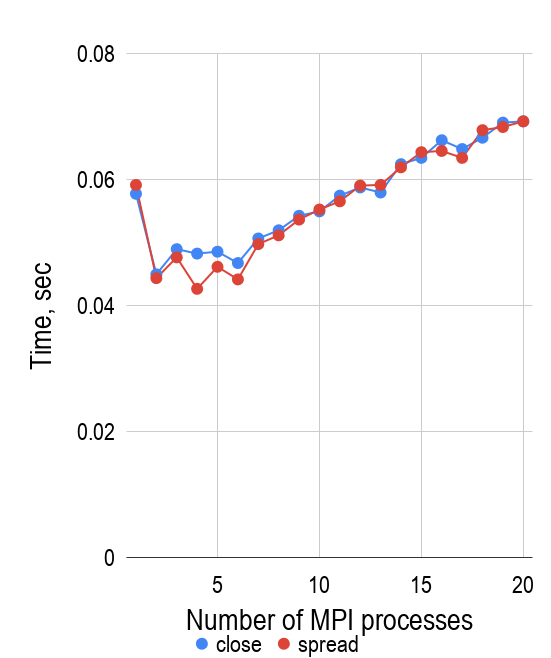
\includegraphics[width=0.48\textwidth]{figures/chapter-2/spread-vs-close/grs-cluster/pwr-3d.png}} &
		\subfloat[HW2 - pwr-3d]{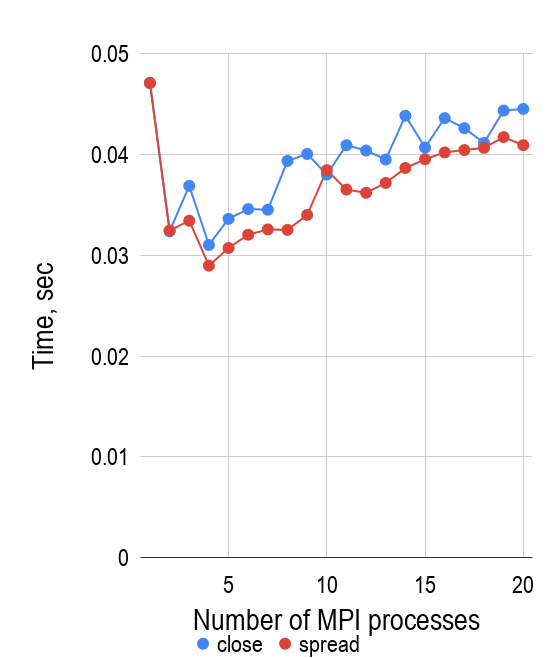
\includegraphics[width=0.48\textwidth]{figures/chapter-2/spread-vs-close/linux-cluster/pwr-3d.png}} \\
		\subfloat[HW1 - cube-64]{\includegraphics[width=0.48\textwidth]{figures/chapter-2/spread-vs-close/grs-cluster/cube-64.png}} &
		\subfloat[HW2 - cube-64]{\includegraphics[width=0.48\textwidth]{figures/chapter-2/spread-vs-close/linux-cluster/cube-64.png}} \\
	\end{tabular}
	\caption{Comparison of \textit{close} and \textit{spread} pinning strategies}
	\label{fig:mumps-close-vs-spread-1}
\end{figure}



\figpointer{\ref{fig:mumps-close-vs-spread-2}}
\begin{figure}[htpb]
\centering
	\begin{tabular}{cc}
		\subfloat[HW1 - cube-645]{\includegraphics[width=0.48\textwidth]{figures/chapter-2/spread-vs-close/grs-cluster/cube-645.png}} &
		\subfloat[HW2 - cube-645]{\includegraphics[width=0.48\textwidth]{figures/chapter-2/spread-vs-close/linux-cluster/cube-645.png}} \\
		\subfloat[HW1 - k3-18]{\includegraphics[width=0.48\textwidth]{figures/chapter-2/spread-vs-close/grs-cluster/k3-18.png}} &
		\subfloat[HW2 - k3-18]{\includegraphics[width=0.48\textwidth]{figures/chapter-2/spread-vs-close/linux-cluster/k3-18.png}} \\
	\end{tabular}
	\caption{Comparison of \textit{close} and \textit{spread} pinning strategies}
	\label{fig:mumps-close-vs-spread-2}
\end{figure}




\figpointer{\ref{fig:mumps-close-vs-spread-3}}
\begin{figure}[htpb]
\centering
	\begin{tabular}{cc}
		\subfloat[HW1 - PFlow\_742]{\includegraphics[width=0.48\textwidth]{figures/chapter-2/spread-vs-close/grs-cluster/PFlow_742.png}} &
		\subfloat[HW2 - PFlow\_742]{\includegraphics[width=0.48\textwidth]{figures/chapter-2/spread-vs-close/linux-cluster/PFlow_742.png}} \\
		\subfloat[HW1 - CurlCurl\_3]{\includegraphics[width=0.48\textwidth]{figures/chapter-2/spread-vs-close/grs-cluster/CurlCurl_3.png}} &
		\subfloat[HW2 - CurlCurl\_3]{\includegraphics[width=0.48\textwidth]{figures/chapter-2/spread-vs-close/linux-cluster/CurlCurl_3.png}} \\
	\end{tabular}
	\caption{Comparison of \textit{close} and \textit{spread} pinning strategies}
	\label{fig:mumps-close-vs-spread-3}
\end{figure}


The tests revealed that \textit{spread}-pinning performed better and allowed to reduce run-time by approximately BRA\% in average in contrast to the \textit{close} strategy. As expected, the points with 1 and 20 MPI processes show the same performance because they basically represent the same process distribution. Additionally, almost BRA\% improvement can be observed around the saturation point in case of \textit{spread} strategy application.\\


Taken into account results of the tests, \textit{spread}-pinning has been chosen for the rest of the study because it shows better overall performance in the intermediate range, in terms of the number MPI processes, where a saturation point can occur. As an example, we would like to point out this process distribution can be particular useful for matrices such as \textit{pwr-3d} and \textit{cube-5} where saturation happens at the number of processes equal to 4.\\


In general, such process distribution can be easily achieved by means of some advanced OpenMPI options, for example \textit{--map-by}, as following:. \\

\begin{lstlisting}[language=bash, caption={An example of \textit{spread}-pinning with using OpenMPI options in case of a flat-MPI run}, frame=single, label={lst:iterative-refinement}]
mpiexec --map-by socket -n $num_proc $executable_name $parameters
\end{lstlisting}



\section{Choice of BLAS Library}
\label{subseq:blas-comparison}


To perform columns elimination of fully summed block of frontal matrices, MUMPS intensively uses GEMM, TRSM and GETRF subroutines which are parts of BLAS and LAPACK libraries. As an example, figure \ref{fig:mumps:steps-of-type-2-factorization} demonstrates factorization of a type 2 node.\\


\figpointer{\ref{fig:mumps:type-2-frontal-matrix}}
\begin{figure}[htpb]
  \centering
  \includegraphics[width=0.45\textwidth]{figures/chapter-2/mumps-type-2-frontal-matrix.png}
\caption{MUMPS: static and dynamic scheduling}
\label{fig:mumps:type-2-frontal-matrix}
\end{figure}


\figpointer{fig:mumps:steps-of-type-2-factorization}
\begin{figure}[htpb]
  \centering
  \includegraphics[width=0.85\textwidth]{figures/chapter-2/mumps-type-2-part-1.png}
\caption{MUMPS: An example of a type 2 node factorization}
\label{fig:mumps:steps-of-type-2-factorization}
\end{figure}


Both BLAS and LAPACK originate from the Netlib project which is a repository of numerous scientific computing software maintained by AT\&T Bell Laboratories, the University of Tennessee, Oak Ridge National Laboratory and other scintific communities \cite{netlib-overview}.\\


The goal of BLAS library is to provide a high efficient implementation of common dense linear algebra kernels by means of high rate of floating point operations per memory access, low cache and Translation Lookaside Buffer (TLB) miss rates.\\


In its turn, LAPACK is designed in such a way so that as much as possible of computation is performed by calls to BLAS library. This allows to achieve high efficiency for operations such as $LU$, $QR$, $SVD$ decompositions, triangular solve, etc. on modern computers. However, the Netlib BLAS implementation is written for an abstract general-purpose central processing unit, in mind, where hardware parameters are based on market statistics. Hence, it is not possible to achieve the maximum possible performance on a specific machine.\\


Hence, there exist special-purpose, hardware-specific implementations of the library developed by hardware vendors i.e. IBM, Cray, Intel, AMD, etc., as well as open-source tuned implementations such as ATLAS, OpenBLAS, etc. To achieve full compatibility, the developers consider the Netlib implementation of BLAS library as the standard (or reference) and thus overwrite all subroutines with additional tuning and optimization. This approach makes it possible to easily replace different BLAS implementations during object files linking  without any modifications of the source code.\\
 

Table \ref{table:list-of-blas-implementations} shows commercial and open-source tunned BLAS implementations available on the market today.\\

\begin{table}[h!]
\centering
\begin{tabular}{|c|c|c|}
\hline
Name                                                                 & Description                                                                                                                                                 & License                                                       \\ \hline
Accelerate                                                           & Apple's implementation for macOS and iOS                                                                                                                    & \begin{tabular}[c]{@{}c@{}}proprietary\\ license\end{tabular} \\ \hline
ACML                                                                 & BLAS implementation for AMD processors                                                                                                                      & \begin{tabular}[c]{@{}c@{}}proprietary\\ license\end{tabular} \\ \hline
C++ AMP                                                              & Microsoft's AMP language extension for Visual C++                                                                                                           & \begin{tabular}[c]{@{}c@{}}open\\ source\end{tabular}         \\ \hline
ATLAS                                                                & Automatically tuned BLAS implementation                                                                                                                     & \begin{tabular}[c]{@{}c@{}}open\\ source\end{tabular}         \\ \hline
Eigen BLAS                                                           & \begin{tabular}[c]{@{}c@{}}BLAS implemented on top of \\ the MPL-licensed Eigen library\end{tabular}                                                        & open source                                                   \\ \hline
ESSL                                                                 & optimized BLAS implementation for  IBM's machines                                                                                                           & \begin{tabular}[c]{@{}c@{}}proprietary\\ license\end{tabular} \\ \hline
GotoBLAS                                                             & Kazushige Goto's implementation of BLAS                                                                                                                     & \begin{tabular}[c]{@{}c@{}}proprietary\\ license\end{tabular} \\ \hline
HP MLIB                                                              & \begin{tabular}[c]{@{}c@{}}BLAS implementation supporting IA-64, PA-RISC, x86 \\ and Opteron architecture\end{tabular}                                      & \begin{tabular}[c]{@{}c@{}}proprietary\\ license\end{tabular} \\ \hline
Intel MKL                                                            & \begin{tabular}[c]{@{}c@{}}Intel's implementation of BLAS optimized for\\ Intel Pentium, Core,  Xeon and Xeon Phi\end{tabular}                              & \begin{tabular}[c]{@{}c@{}}proprietary\\ license\end{tabular} \\ \hline
Netlib BLAS                                                          & The official reference implementation on Netlib                                                                                                             & \begin{tabular}[c]{@{}c@{}}open\\ source\end{tabular}         \\ \hline
OpenBLAS                                                             & Optimized BLAS library based on GotoBLAS                                                                                                                    & \begin{tabular}[c]{@{}c@{}}open\\ source\end{tabular}         \\ \hline
PDLIB/SX                                                             & BLAS library targeted to the NEC SX-4 system                                                                                                                & \begin{tabular}[c]{@{}c@{}}proprietary\\ license\end{tabular} \\ \hline
SCSL                                                                 & BLAS implementations for SGI's Irix workstations                                                                                                            & \begin{tabular}[c]{@{}c@{}}proprietary\\ license\end{tabular} \\ \hline
\begin{tabular}[c]{@{}c@{}}Sun\\ Performance \\ Library\end{tabular} & \begin{tabular}[c]{@{}c@{}}Optimized BLAS and LAPACK for SPARC, Core \\ and AMD64 architectures under \\ Solaris 8, 9, and 10 as well as Linux\end{tabular} & \begin{tabular}[c]{@{}c@{}}proprietary\\ license\end{tabular} \\ \hline
\end{tabular}
\caption{Comerrcial and open source BLAS implementations \cite{wiki:blas-implementations}}
\label{table:list-of-blas-implementations}
\end{table}



Among all libraries listed in table \ref{table:list-of-blas-implementations} there were only four available on HW1 machine, namely: Netlib BLAS, Intel MKL, OpenBLAS and ATLAS. However, installation of ATLAS requires to switch off dynamic frequency scaling, also called CPU throttling, to allow an ATLAS configuration routine to find the best loop transformation parameters for a specific hardware. In order to turn off CPU throttling, one has to reboot the entire machine and make appropriate changes in Basic Input/Output System (BIOS). This fact made ATLAS library not to be suitable for the rest of the research and we excluded it from our primary list of candidates. Moreover, during installation, one has to explicitly provide the number of OpenMP threads that are going to be used once a BLAS subroutine is called. This means there is no way to change the number of threads per MPI process in run-time without re-installation of ATALS library. Thus, only 3 versions of MUMPS-PETSc (Netlib BLAS, Intel MKL and OpenBLAS) libraries were compiled and tested with using GRS matrix set and 1 thread per MPI process. The test results are shown in figures bla, bla and bra.\\



% say that ATLAS is shit and we have to live only with Intel MKL and OpenBlas

% Say that we are going to use Netlib blas as the baseline


\subsection{\gls{mpi}-\gls{openmp} Tuning of \gls{mumps} Library}
\label{subseq:mpi-openmp}


As it was mentioned in subsection \ref{subseq:mumps-review}, the development of \gls{mumps} began in 1996 when message-passing programming paradigm dominated in parallel computing. Therefore, the library originally was designed only for distributed-memory machines.\\

In 2010,  \citeauthor{chowdhury2010some} published their first experiments and some issues, in \cite{chowdhury2010some}, of exploiting shared memory parallelism in \gls{mumps}. The authors showed that it was possible to achieve some improvements in multicore systems using multi-threading, given a purely \gls{mpi} application. However, later \citeauthor{l2013introduction} mentioned, in \cite{l2013introduction}, that adaptation of the existing code for \gls{numa} architecture was still a challenge because of memory allocation, memory affinity, thread pinning and other related issues.\\


In spite of an advantage of natural data locality of message-passing applications, a general motivation for switching to a hybrid mode, a mixed \gls{mpi}/\gls{openmp} process/thread distribution, is to reduce communication overheads between \gls{mpi} processes. According to the profiling results done by \citeauthor{chowdhury2010some}, \gls{mumps} contained four main regions of shared-memory parallelization, namely: 

\begin{enumerate}

	\item \gls{blas} Level 1, 2, 3 operations during both factorization and solution phases \label{openmp-blocks-1}
	
	\item Assembly operations, where contribution blocks of children nodes are assembled at the parent level \label{openmp-blocks-2}
	
	\item Copying contribution blocks during stacking operations \label{openmp-blocks-3}
	
	\item Pivot search operations \label{openmp-blocks-4}

\end{enumerate}


Almost all customized \gls{blas} libraries, for example Intel MKL and OpenBLAS, are multi-threaded and can efficiently work in shared-memory environment. Hence, parallelization of region \ref{openmp-blocks-1} can be achieved by linking a suitable \gls{blas} library whereas regions \ref{openmp-blocks-2}, \ref{openmp-blocks-3} and \ref{openmp-blocks-4} can be multi-threaded by inserting appropriate \gls{openmp} directives above the corresponding loop statements.\\


A detailed review of works \cite{l2013introduction} and \cite{chowdhury2010some} reveals that, in general, a pure \gls{openmp} or mixed \gls{mpi}/\gls{openmp} strategy can reduce run-time of \gls{mumps}. On average, factorization time is reduced by \textbf{14.3\%} and in some special cases improvements reach about \textbf{50.4\%}, according to the data provided in the papers. However, at the same time, the results also show that sometimes flat-\gls{mpi} mode can significantly outperform other hybrid mixed strategies.\\


By and large, the results show two important aspects. Firstly, performance of a specific strategy depends heavily on a resulting assembly tree and thus on a matrix sparsity pattern and applied fill reducing reordering. Secondly, it is not possible to guess in advance which strategy gives the best parallel performance without detailed information about the tree structure and computational cost per node. \citeauthor{l2013introduction} showed that performance of a particular mode dependeds on a ratio of large and small fronts. For example, they noticed that more threads per \gls{mpi} process resulted in better parallel performance when the ratio was high. On the other hand, they observed the absolutely opposite result with relatively small ratios. Unfortunately, \citeauthor{l2013introduction} did not provide any quantitative measure for the notion of small and large ratios in their work \cite{l2013introduction}.\\ 


It is also interesting to notice that parallelization of region 1 using a multi-threaded \gls{blas} library gives the most of the parallel performance improvement for mixed or pure \gls{openmp} strategies, according to the results from \cite{l2013introduction}. Whereas,
multi-threading of regions 2, 3, 4 has only a small positive effect i.e it reduces numerical factorization run-time by only \textbf{0.66\%} on an average.\\



This outcome is expected because \gls{blas} subroutines, especially level 3, re-use data stored in caches as much as possible and thus achieve high ratios of floating point operations per memory access which is essential for efficient multi-threading. Meanwhile, regions 2, 3, 4 mainly perform initialization of variables, data movements and executions of \textit{if-statements} which always result in low computational intensity.\\

%\todo{consider that paragraph}
%Additionally, it is worth noticing that both works, \cite{chowdhury2010some} and \cite{l2013introduction}, were mainly focused on the numerical factorization phase assuming that both analysis and solution phases do not take lots of computational time. In spite of credibility of this assumption, it still should be pointed out the solution phase runs faster in case of flat-\gls{mpi} mode. This fact becomes even more interesting because, in our case, a system with multiple right-hand sides has to be solved in order to generate a preconditioner.\\


We have to admit that both works, \cite{chowdhury2010some} and \cite{l2013introduction}, are relatively old and the analysis above may be not complete and full. Because \gls{mumps} is a dynamic developing project, we can expect that adaptation of shared-memory parallelization in \gls{mumps} has been significantly advanced since that time. Since the 4-th release of \gls{mumps} library, the developers have persistently recommended to use only hybrid strategies e.g. \textit{one \gls{mpi} process per socket and as many threads as the number of cores} \cite{mumps-manual}.\\


As an initial test, we compared influence of both Intel MKL and OpenBLAS libraries on parallel performance of \gls{mumps} using \gls{grs} matrix set only. In order to pin \gls{openmp} threads in a correct way, without any conflicts between them, the following \gls{openmp} environment variables were set as follows:

\begin{itemize}
	\item OMP\_PLACES=cores
	\item OMP\_PROC\_BIND=spread
\end{itemize} 


During the testing, we found that sometimes execution time of \gls{mumps}-OpenBLAS configuration abnormality increased. For instance, in case of factorization of matrix \textit{cube-645}, the increase reached almost \textbf{450\%} in contrast to the pure sequential execution. \\

\figpointer{\ref{fig:mumps-openblas-anomalies}}
\begin{figure}[htpb]
\centering
	\begin{tabular}{cc}
		\subfloat[k3-18]{\includegraphics[width=0.4\textwidth]{figures/chapter-2/openmp-mpi/anomalies-k3-18.png}} &
		\subfloat[cube-645]{\includegraphics[width=0.4\textwidth]{figures/chapter-2/openmp-mpi/anomalies-cube-645.png}} \\
	\end{tabular}
	\caption{Anomalies of \gls{mumps}-OpenBLAS configuration running with 2 \gls{openmp} threads per \gls{mpi} process}
	\label{fig:mumps-openblas-anomalies}
\end{figure}


Multiple conflicts between application and system threads were observed using \textit{htop} software as an interactive process viewer. Figure \ref{fig:mumps:openblas-thread-conflcit} shows a snapshot taken during factorization of matrix \textit{k3-18} running with 1 \gls{mpi} process and 20 threads.\\


\figpointer{\ref{fig:mumps:openblas-thread-conflcit}}
\begin{figure}[htpb]
  \centering
  \includegraphics[width=0.75\textwidth]{figures/chapter-2/openmp-mpi/thread-conflict.png}
\caption{A \gls{mumps}-OpenBLAS thread conflict in case of \textit{k3-18} matrix factorization (green - application threads, red - system threads)}
\label{fig:mumps:openblas-thread-conflcit}
\end{figure}


It is difficult to state what exactly caused such behavior. However, \citeauthor{chowdhury2010some} also reported about the same problem using GotoBLAS (OpenBLAS). They assumed that GotoBLAS created and kept some threads active even after the main threads returned to the calling application which could lead to interference with threads created in other \gls{openmp} regions \cite{chowdhury2010some}. For this reason, we decided to use only Intel MKL library for the rest of the study because there were no such thread-conflicts detected during operation of \gls{mumps}-Intel MKL configuration.\\


Only common mixed \gls{mpi}/\gls{openmp} strategies were tested in order to check influence of shared-memory parallelism on parallel performance of \gls{mumps} as well as to limit the amount of testing. The following strategies were chosen: 20 \gls{mpi} - 1 thread (flat-\gls{mpi}), 10 \gls{mpi} - 2 threads, 4 \gls{mpi} - 5 threads, 2 \gls{mpi} - 10 threads, 1 \gls{mpi} - 20 threads (flat-\gls{openmp}). The tests were conducted on both \gls{hw1} and \gls{hw2} machines with the aim of checking whether  results would be consistent between different hardware running under different operating and environment settings. The test results are represented in tables \ref{fig:mpi-omp-grs-hw1} \ref{fig:mpi-omp-grs-hw2}, \ref{fig:mpi-omp-suitesparse-hw1} and \ref{fig:mpi-omp-suitesparse-hw2} where numerical values are given in seconds.\\


%%%%%%%%%%%%%%%%%%%%%%%%%%%%%%%%%%%%%%%%%%%%%%%%%%%%
\begin{table}[h!]
\centering
\begin{tabular}{|c|c|c|c|c|c|c|}
\hline
\begin{tabular}[c]{@{}c@{}}Matrix\\ Name\end{tabular} & \begin{tabular}[c]{@{}c@{}}20 MPI\\ 1 thread\end{tabular} & \begin{tabular}[c]{@{}c@{}}10 MPI\\ 2 threads\end{tabular} & \begin{tabular}[c]{@{}c@{}}4 MPI\\ 5 threads\end{tabular} & \begin{tabular}[c]{@{}c@{}}2 MPI\\ 10 threads\end{tabular} & \begin{tabular}[c]{@{}c@{}}1 MPI\\ 20 threads\end{tabular} & \begin{tabular}[c]{@{}c@{}}Gain\\ w.r.t.\\ flat-MPI\end{tabular} \\ \hline
k3-18                                                 & \textbf{12.520}                                           & 12.630                                                     & 14.010                                                    & 18.020                                                     & 19.170                                                     & -                                                                \\ \hline
k3-2                                                  & 1.341                                                     & \textbf{1.250}                                             & 1.470                                                     & 1.671                                                      & 2.052                                                      & 1.073                                                            \\ \hline
cube-645                                              & \textbf{6.585}                                            & 6.859                                                      & 8.552                                                     & 12.010                                                     & 14.080                                                     & -                                                                \\ \hline
cube-64                                               & 0.756                                                     & \textbf{0.749}                                             & 0.874                                                     & 1.178                                                      & 1.354                                                      & 1.010                                                            \\ \hline
cube-5                                                & 0.181                                                     & 0.132                                                      & \textbf{0.104}                                            & 0.126                                                      & 0.117                                                      & 1.744                                                            \\ \hline
pwr-3d                                                & 0.130                                                     & 0.114                                                      & 0.0972                                                    & \textbf{0.077}                                             & 0.109                                                      & 1.691                                                            \\ \hline
\end{tabular}
\caption{Compassion of different hybrid \gls{mpi}/\gls{openmp} modes used for \gls{grs} matrix set on \gls{hw1}}
\label{fig:mpi-omp-grs-hw1}
\end{table}



\begin{table}[h!]
\centering
\begin{tabular}{|c|c|c|c|c|c|c|}
\hline
\begin{tabular}[c]{@{}c@{}}Matrix\\ Name\end{tabular} & \begin{tabular}[c]{@{}c@{}}20 MPI\\ 1 thread\end{tabular} & \begin{tabular}[c]{@{}c@{}}10 MPI\\ 2 threads\end{tabular} & \begin{tabular}[c]{@{}c@{}}4 MPI\\ 5 threads\end{tabular} & \begin{tabular}[c]{@{}c@{}}2 MPI\\ 10 threads\end{tabular} & \begin{tabular}[c]{@{}c@{}}1 MPI\\ 20 threads\end{tabular} & \begin{tabular}[c]{@{}c@{}}Gain\\ w.r.t.\\ flat-MPI\end{tabular} \\ \hline
k3-18                                                 & 8.558                                                     & \textbf{7.819}                                             & 8.165                                                     & 11.330                                                     & 14.320                                                     & 1.095                                                            \\ \hline
k3-2                                                  & 1.168                                                     & \textbf{0.788}                                             & 0.956                                                     & 1.131                                                      & 1.651                                                      & 1.482                                                            \\ \hline
cube-645                                              & 5.735                                                     & \textbf{4.859}                                             & 6.069                                                     & 9.360                                                      & 11.040                                                     & 1.180                                                            \\ \hline
cube-64                                               & 0.805                                                     & \textbf{0.541}                                             & 0.664                                                     & 0.947                                                      & 0.918                                                      & 1.490                                                            \\ \hline
cube-5                                                & 0.241                                                     & 0.121                                                      & \textbf{0.093}                                            & 0.129                                                      & 0.126                                                      & 2.582                                                            \\ \hline
pwr-3d                                                & 0.234                                                     & 0.095                                                      & 0.098                                                     & \textbf{0.070}                                             & 0.094                                                      & 3.341                                                            \\ \hline
\end{tabular}
\caption{Compassion of different hybrid \gls{mpi}/\gls{openmp} modes used for \gls{grs} matrix set on \gls{hw2}}
\label{fig:mpi-omp-grs-hw2}
\end{table}


%%%%%%%%%%%%%%%%%%%%%%%%%%%%%%%%%%%%%%%%%%%%%%%%%%%%
\begin{table}[h!]
\centering
\begin{tabular}{|c|c|c|c|c|c|c|}
\hline
\begin{tabular}[c]{@{}c@{}}Matrix\\ Name\end{tabular} & \begin{tabular}[c]{@{}c@{}}20 MPI\\ 1 thread\end{tabular} & \begin{tabular}[c]{@{}c@{}}10 MPI\\ 2 threads\end{tabular} & \begin{tabular}[c]{@{}c@{}}4 MPI\\ 5 threads\end{tabular} & \begin{tabular}[c]{@{}c@{}}2 MPI\\ 10 threads\end{tabular} & \begin{tabular}[c]{@{}c@{}}1 MPI\\ 20 threads\end{tabular} & \begin{tabular}[c]{@{}c@{}}Gain\\ w.r.t.\\ flat-MPI\end{tabular} \\ \hline
cant                                                  & 1.400                                                     & \textbf{0.990}                                             & 1.050                                                     & 1.605                                                      & 2.019                                                      & 1.414                                                            \\ \hline
consph                                                & 3.495                                                     & \textbf{2.652}                                             & 3.015                                                     & 3.706                                                      & 3.714                                                      & 1.318                                                            \\ \hline
memchip                                               & \textbf{7.470}                                            & 9.080                                                      & 13.301                                                    & 20.198                                                     & 45.800                                                     & -                                                                \\ \hline
PFlow\_742                                            & 26.802                                                    & 24.204                                                     & \textbf{21.897}                                           & 30.389                                                     & 54.501                                                     & 1.224                                                            \\ \hline
pkustk10                                              & \textbf{0.748}                                            & 0.879                                                      & 0.972                                                     & 1.459                                                      & 1.280                                                      & -                                                                \\ \hline
torso3                                                & \textbf{3.922}                                            & 4.285                                                      & 4.642                                                     & 5.603                                                      & 8.144                                                      & -                                                                \\ \hline
x104                                                  & \textbf{1.597}                                            & 1.644                                                      & 2.024                                                     & 3.208                                                      & 2.167                                                      & -                                                                \\ \hline
CurlCurl\_3                                           & 49.250                                                    & 44.120                                                     & \textbf{39.909}                                           & 43.311                                                     & 63.001                                                     & 1.234                                                            \\ \hline
Geo\_1438                                             & 478.101                                                   & 234.697                                                    & \textbf{151.603}                                          & 157.697                                                    & 158.102                                                    & 3.154                                                            \\ \hline
\end{tabular}
\caption{Compassion of different hybrid \gls{mpi}/\gls{openmp} modes used for SuiteSparse matrix set on \gls{hw1}}
\label{fig:mpi-omp-suitesparse-hw1}
\end{table}




\begin{table}[h!]
\centering
\begin{tabular}{|c|c|c|c|c|c|c|}
\hline
\begin{tabular}[c]{@{}c@{}}Matrix\\ Name\end{tabular} & \begin{tabular}[c]{@{}c@{}}20 MPI\\ 1 thread\end{tabular} & \begin{tabular}[c]{@{}c@{}}10 MPI\\ 2 threads\end{tabular} & \begin{tabular}[c]{@{}c@{}}4 MPI\\ 5 threads\end{tabular} & \begin{tabular}[c]{@{}c@{}}2 MPI\\ 10 threads\end{tabular} & \begin{tabular}[c]{@{}c@{}}1 MPI\\ 20 threads\end{tabular} & \begin{tabular}[c]{@{}c@{}}Gain\\ w.r.t\\ flat-MPI\end{tabular} \\ \hline
cant                                                  & 2.128                                                     & \textbf{0.955}                                             & 1.011                                                     & 1.577                                                      & 2.058                                                      & 2.229                                                           \\ \hline
consph                                                & 3.840                                                     & \textbf{2.852}                                             & 3.111                                                     & 3.695                                                      & 3.897                                                      & 1.346                                                           \\ \hline
memchip                                               & \textbf{7.811}                                            & 7.816                                                      & 9.811                                                     & 15.160                                                     & 31.969                                                     & -
\\ \hline
PFlow\_742                                            & 24.190                                                    & 29.241                                                     & \textbf{19.686}                                           & 27.530                                                     & 55.431                                                     & 1.230                                                           \\ \hline
pkustk10                                              & 1.373                                                     & \textbf{0.904}                                             & 1.022                                                     & 1.421                                                      & 1.403                                                      & 1.520                                                           \\ \hline
torso3                                                & 4.733                                                     & \textbf{4.080}                                             & 4.483                                                     & 5.648                                                      & 8.217                                                      & 1.160                                                           \\ \hline
x104                                                  & 2.676                                                     & \textbf{1.597}                                             & 2.025                                                     & 3.204                                                      & 2.133                                                      & 1.676                                                           \\ \hline
CurlCurl\_3                                           & 39.890                                                    & \textbf{34.579}                                            & 38.620                                                    & 41.171                                                     & 67.760                                                     & 1.154                                                           \\ \hline
Geo\_1438                                             & ROM                                                       & ROM                                                        & ROM                                                       & ROM                                                        & ROM                                                        & ROM                                                             \\ \hline
\end{tabular}
\caption{Compassion of different hybrid \gls{mpi}/\gls{openmp} modes used for SuiteSparse matrix set on \gls{hw2}\\
*ROM - run out of memory}
\label{fig:mpi-omp-suitesparse-hw2}
\end{table}


%According to the results, we have noticed the optimal hybrid \gls{mpi}/\gls{openmp} mode locates near the saturation point of the corresponding flat-\gls{mpi} test. Therefore, search of an optimal mode can take considerable amount of time. It is needless to say that the mode varies from matrix to matrix and there is no way to predict the mode in advance. Moreover, the results show that performance gain is around \textbf{2.1\%} in case of \gls{grs} matrix set on \gls{hw1} hardware, excluding small test cases such as \textit{cube-5} and \textit{pwr-3d} where runs with 20 \gls{mpi} processes were slower in contrast to sequential execution. Much optimistic results were obtained for experiments conducted on \gls{hw2} machine were performance gain reached almost \textbf{31\%} for the same test cases.\\


According to the results, we have noticed that an optimal hybrid \gls{mpi}/\gls{openmp} mode locates near the saturation point of the corresponding flat-\gls{mpi} test. Generally speaking, a location of the saturation point is specific for each matrix and, therefore, there is no way to predict a mode in advance. However, having known the point, the amount of testing can be considerably reduced by searching around and applying different mixed \gls{mpi}/\gls{openmp} strategies.\\


The results show that average performance gain is around \textbf{2.1\%} in case of \gls{grs} matrix set for \gls{hw1} hardware, excluding small test-cases such as \textit{cube-5} and \textit{pwr-3d} from statistics. We consider these two scenarios, \textit{cube-5} and \textit{pwr-3d}, as specific ones because their execution time with 20 \gls{mpi} processes using flat-\gls{mpi} mode is originally slower in contrast to the sequential execution and, therefore, it is relevant to assume the improvement came only from reducing the \gls{mpi} process count. At the same time, much optimistic results were obtained from experiments conducted on \gls{hw2} machine where performance gain reached almost \textbf{31\%} for the same test-cases.\\



Results obtained with SuiteSparse matrix set demonstrate much better performance improvements from hybrid parallel computing obtained on both hardware. On average, execution time improves by more than \textbf{15\%} running tests on \gls{hw1} and approximately by \textbf{41\%} on \gls{hw2}, excluding \textit{Geo\_1438} from the statistics. The best result was obtained exactly in case of \textit{Geo\_1438} test-case on both machines where execution time dropped about \textbf{3 times} for all hybrid modes in contrast to the corresponding flat-\gls{mpi} one. We assume it may occur because a high ratio of large and small fronts of this particular test-case.\\


According to the outcomes of testing, we have observed a negligible improvement in \gls{mumps} parallel performance from the application of the multi-threaded Intel MKL \gls{blas} library to \gls{grs} matrix set. Such unimpressive results can be explained with the same reasoning given in subsection \ref{subseq:blas-comparison} i.e. lack of type 2 nodes. Moreover, in case of \gls{grs} matrix set, parallel efficiency drops significantly probably due to inefficient utilization of additional processing elements i.e cores. However, at the same time, results obtained from SuiteSparse matrix set have shown an advantage of hybrid parallel computing, especially in case of \textit{Geo\_1438} matrix factorization.\\


These contradictory results obtained from two different matrix sets second our reasoning of specifics of linear systems generated by \gls{athlet} software. Again, we presume that assembly trees resulted from \gls{grs} matrices are mostly formed with subtrees filled with type 1 nodes where each subtree is processed by single \gls{mpi} process. Hence, parallel factorization of \gls{grs} matrices mainly gets benefit from \gls{mpi} parallelization that can be clearly observed from the results.\\



In this subsection, we have discussed how \gls{mumps} adopts hybrid parallel programming. As it is in case of fill reducing reordering algorithm selection, subsection \ref{subseq:fill-in-reordering}, it is not possible to find an optimal mixed \gls{mpi}/\gls{openmp} strategy in advance without performance testing. We have come to the concluded that flat-\gls{mpi} mode is the best one for \gls{grs} matrix set and provided our reasoning for that. Generally speaking, there are 3 reason to use this mode in our case. Firstly, the mode always resulted in more efficient hardware utilization. Secondly, the improvements obtained with \gls{mumps}-Intel MKL configuration running with optimal hybrid \gls{mpi}/\gls{openmp} modes can deteriorate performance gain obtained with \gls{mumps}-OpenBLAS flat-\gls{mpi} configuration, shown in subsection \ref{subseq:blas-comparison}. Finally, efficient utilization of flat-\gls{mpi} strategy only demands to find an optimal \gls{mpi} process count i.e the saturation point on a performance graph. Hence, it leads to significant reduction of amount of testing. \\


	\section{Results}
	\label{subseq:final-results}


Figures \ref{fig:mumps-final-comparison-1} and \ref{fig:mumps-final-comparison-2} show comparisons of MUMPS parallel performance before and after application of the optimal MUMPS settings, found in subsections \ref{subseq:fill-in-reordering}, \ref{subseq:mm-mumps-process-pinning}, \ref{subseq:blas-comparison}, and \ref{subseq:mpi-openmp}, to GRS matrix set. Results labeled as \textit{default} were obtained using the fill reducing reordering algorithm provided by ParMetis library because it had been used by ATHLET users before the current study.\\


%\figpointer{\ref{fig:mumps-final-comparison-1}}
\begin{figure}[h!]
\centering
	\begin{tabular}{cc}
		\subfloat[small system: cube-5\label{fig:mumps-final-comparison-cube-5}]{\includegraphics[width=0.41\textwidth]{figures/chapter-2/final-comparison/cube-5.png}} &
		\subfloat[small system: pwr-3d\label{fig:mumps-final-comparison-pwr-3d}]{\includegraphics[width=0.41\textwidth]{figures/chapter-2/final-comparison/pwr-3d.png}} \\
		\subfloat[medium system: cube-64]{\includegraphics[width=0.41\textwidth]{figures/chapter-2/final-comparison/cube-64.png}} & 			        \subfloat[medium system: k3-2]{\includegraphics[width=0.41\textwidth]{figures/chapter-2/final-comparison/k3-2.png}} \\
	\end{tabular}
	\caption{Comparison of MUMPS parallel performance before and after application of optimal settings to small- and middle-sized GRS problems}
	\label{fig:mumps-final-comparison-1}
\end{figure}



%\figpointer{\ref{fig:mumps-final-comparison-2}}
\begin{figure}
\centering
	\begin{tabular}{cc}
		\subfloat[large system: cube-645\label{fig:mumps-final-comparison-cube-645}]{\includegraphics[width=0.43\textwidth]{figures/chapter-2/final-comparison/cube-645.png}} & 			        \subfloat[large system: k3-18\label{fig:mumps-final-comparison-k3-18}]{\includegraphics[width=0.43\textwidth]{figures/chapter-2/final-comparison/k3-18.png}} \\
	\end{tabular}
	\caption{Comparison of MUMPS parallel performance before and after application of optimal settings to large-sized GRS problems}
	\label{fig:mumps-final-comparison-2}
\end{figure}

\newpage



On average, factorization time is reduced by \textbf{51.4\%} for small-sized linear systems, \textit{cube-5} and \textit{pwr-3d}. As it was expected, the most significant performance gain mainly comes from a correct choice of a fill reducing reordering algorithm. Moreover, application of PT-Scotch for these systems of equations results in a drastic change of strong scaling behavior, see figures \ref{fig:mumps-final-comparison-cube-5} and  \ref{fig:mumps-final-comparison-pwr-3d}, which allows to reduce execution time by approximately \textbf{17\%} in contrast to the sequential execution of MUMPS running with the default parameters.\\


% medium sized systems
Execution time spent on factorization of medium-sized systems, such as \textit{cube-64} and \textit{k3-2}, drops in \textbf{1.4} times on an average. We have noticed that strong scaling of \textit{cube-64} test-case considerably improves. Additionally, application of PT-Scotch to \textit{cube-64} matrix results in shifting of the optimal MPI process count, the saturation point, from 5 to 10 and, as a result, it improves efficiency of the solver. Applied settings reduce execution time around the corresponding saturation points by almost \textbf{31\%} on average for these type of GRS matrices.\\


% larged sized sized system
%Only optimal processes pinning and application of OpenBLAS library result in parallel performance gain of large-sized systems because of usage of the same fill reducing reordering algorithm, ParMetis.

Improvements in parallel factorization of large-sized GRS systems comes only from optimal processes pinning and application of OpenBLAS library because of the usage of the same optimal fill reducing reordering algorithm, ParMetis. On average, performance increased almost by \textbf{20\%} in case of \textit{k3-18} test-case and only by \textbf{1.3\%} for \textit{cube-645} one. This difference in results can be explained by the fact that the assembly tree of \textit{cube-645} test-case lacks type 2 nodes. However, the saturation points of both test-cases are shifted towards lower values of the MPI process count which results in a considerably improvement of hardware utilization. For example, a detailed study of \textit{k3-18} performance graph, figure \ref{fig:mumps-final-comparison-k3-18}, shows the optimal MPI process count value decreases from 17 to 8 and, at the same time, execution time drops by almost \textbf{19\%}. These two effects result in almost \textbf{13\%} jump of parallel efficiency. The same trend can be observed for \textit{cube-645} test-case as well.\\


By and large, in this subsection we have shown the application of the optimal parameters to MUMPS leads to total accumulative improvements in factorization time and hardware utilization.\\



%average
% shit of saturation point
% usage of less amount of processing units helps to improve efficiency of the system
% example of k-18, k3-2
% recomendations for small, medium and big GRS systems


	\section{Conclusion}
	\label{subseq:mm-conclusion}

In this chapter, we have examined different types of sparse linear solvers applied to linear systems generated by \acrshort{athlet} software resulting from numerical integration of thermo-hydraulic computations. We have come to the conclusion that, in spite of better scalability and parallel efficiency of iterative methods due to efficient data-based parallelism, direct sparse linear solvers are much suitable for this purpose because of their robustness, see Subsection \ref{subseq:hybrid-method-description}.\\


In Subsection \ref{subseq:mm-library-choice}, we tested different direct sparse solvers, namely: \acrshort{mumps},  SuperLU\_DIST and PasTiX. \acrshort{mumps} showed better parallel performance among the others according to  the results of testing and, therefore, was chosen for the following study where we mainly focused on performance tuning of the library.\\


We have shown in subsequent subsections there have been four main sources of library parameter tuning, namely:

\begin{enumerate}
	\item correct selection of a fill reducing reordering algorithm \label{conclusion:mm-1}
	\item destribution of \acrshort{mpi} processes among multiple \acrshort{numa} domain within a compute node \label{conclusion:mm-2}
	\item configuration of \acrshort{mumps} with an optimal, tuned \acrshort{blas} library implementaion \label{conclusion:mm-3}
	\item execution of \acrshort{mumps} with optimal hybrid \acrshort{mpi}/\acrshort{openmp} process/thread distributions \label{conclusion:mm-4}
\end{enumerate}


Testing was performed using two different matrix set, \acrshort{grs} and SuiteSparse, on two different computer-clusters, \gls{hw1} and \gls{hw2}, see Chapter \ref{subseq:matrix-sets-and-hardware}, in order to check consistency of obtained results. In this subsection, we  give most general conclusions relevant to only \acrshort{grs} matrix set and \gls{hw1} cluster as targets of the study. The reader can become familiar with detailed conclusions relative to both matrix sets and hardware given at the end of each subsection that we are going to reference to.\\



\ref{conclusion:mm-1}. In Subsection \ref{subseq:fill-in-reordering}, it has been shown that parallel performance of \acrshort{mumps} is quite sensitive to an applied fill-in reducing reordering algorithm. A correct choice of the algorithm can lead to a significant improvement in execution time and strong scaling behavior. We have noticed that \acrshort{mumps} performs factorizations of small- and medium-sized matrices faster using PT-Scotch library whereas large-sized problems tend to get benefit from the algorithm provided by ParMetis. We assume the obtained conclusion may be not accurate due to a small size of \acrshort{grs} matrix set. At the moment of writing, we have not found any indirect metric to predict a correct choice of an algorithm beforehand. Thus, we encourage \acrshort{athlet} users to perform similar testing described in the subsection before running thermo-hydraulic simulations on distributed-memory machines to achieve better performance of parallel computations.\\




%%%%%%%%%%%%%%%%%%%%%%%%%%%%%%%%%%%%%%%%%%%%%%
\ref{conclusion:mm-2}. In Subsection \ref{subseq:mm-mumps-process-pinning}, an influence of different process pinning strategies on \acrshort{mumps} parallel performance has been investigated. The tests have shown that an equal distribution of \acrshort{mpi} process among all available \acrshort{numa} domains always results in additional performance gain.\\ %On average, \textit{spread}-pinning allows to reduce execution time of \acrshort{mumps} by almost \textbf{5.5\%} and \textbf{13.8\%} on \gls{hw1} and \gls{hw2} machines, respectively.\\


%%%%%%%%%%%%%%%%%%%%%%%%%%%%%%%%%%%%%%%%%%%%%%
\ref{conclusion:mm-3}. 
In Subsection \ref{subseq:blas-comparison},
we tested \acrshort{mumps} configured with 3 different implementations of \acrshort{blas} library, namely: Netlib, OpenBLAS and Intel MKL. The results have shown the application of OpenBLAS library always results in better parallel performance.\\


%Comparison and analysis of results obtained from \acrshort{grs} and SuiteSparse matrix sets allows to make an assumption that matrices generated by \acrshort{athlet} software are specific, probably due to specifics of spacial and time integration, and results in assembly trees with low number of type 2 nodes.

% we have discussed and examined a way how \acrshort{mumps} preforms partial factorizations of type 2 nodes utilizing \acrshort{blas} and \acrshort{lapack} subroutines. We have tested \acrshort{mumps} linked with 3 different implementations of BLAS: (default) Netlib, Intel MKL and OpenBLAS. The results have shown that replacement the default \acrshort{blas} implementation with a tuned one usually results in improvement of the overall solver performance. However, we have observed that degree of improvement significantly varies between test-cases. We have assumed that it may depend on the assembly tree structure of a specific test-case i.e. the ratio between type 2 and type 1 nodes.\\

%By and large, the results have shown that OpenBLAS outperforms both Netlib and Intel MKL libraries in case of \acrshort{grs} matrix set. On an average, \acrshort{mumps}-OpenBLAS configuration was about \textbf{13\%} and \textbf{21\%} faster than \acrshort{mumps}-Intel MKL and the default \acrshort{mumps}-Netlib configurations, respectively.\\


%%%%%%%%%%%%%%%%%%%%%%%%%%%%%%%%%%%%%%%%%%%%%%
	
\ref{conclusion:mm-4}. In Subsection \ref{subseq:mpi-openmp}, we have investigated an impact of various
\acrshort{mpi}/\acrshort{openmp} process/thread distributions on parallel factorizations of \acrshort{grs} matrices  within a compute-node. We have observed that multi-threading of
OpenBLAS library in \acrshort{mumps} leads to multiple thread conflicts which sometimes result in significant slow-down of the solver. Results obtained with \acrshort{mumps}-Intel MKL configuration have demonstrated a negligible improvement in solver execution time resulting in a significant parallel efficiency drop, probably due to inefficient usage of additional processing elements utilized by forked Intel MKL threads. At the end, we have concluded that flat-\acrshort{mpi} mode is the best one for matrices generated by \acrshort{athlet} software.\\




%discussed how and where \acrshort{mumps} library make use of shared-memory parallelism based on review of works \cite{chowdhury2010some} and \cite{l2013introduction} \todo{problems with open blas} \todo{intel mkl}. We have also found severe slow-down of some hybrid \acrshort{mpi}/\acrshort{openmp} modes due to system and application thread conflicts  while \acrshort{mumps}-\acrshort{openmp} configuration was running on \gls{hw1} cluster. For that reason, the following study was continued with only using Intel MKL library which, in its turn, turned out to be thread-safe.\\


%We have shown that in some particular cases, factorization of \textit{Geo\_1438} matrix for example, hybrid \acrshort{mpi}-\acrshort{openmp} approach can bring significant performance improvement. However, application of hybrid computing to \acrshort{grs} matrix set gives negligible improvement on \gls{hw1} machine i.e. around \textbf{2.1\%}, and significantly deteriorates parallel efficiency. Much optimistic results were obtained for experiments conducted on \gls{hw2} machine were performance gain reached almost \textbf{31\%} for the same matrix set. \\


%During the study, we have also discovered the optimal hybrid \acrshort{mpi}/\acrshort{openmp} mode locates near the saturation point of the corresponding flat-\acrshort{mpi} test. This fact can allow to reduce the amount of testing in general. However, we do not recommend to proceed the study in this direction due to above mention parallel efficiency issues detected on \gls{hw1} machine and lack of ability to run Open\acrshort{blas} library without thread conflicts.\\


In Subsection \ref{subseq:final-results}, we have studied the overall impact of introduced configuration changes found in Subsections \ref{subseq:fill-in-reordering}, \ref{subseq:mm-mumps-process-pinning}, \ref{subseq:blas-comparison} and \ref{subseq:mpi-openmp}. Testing shows the changes result in a positive accumulative effect leading to considerable improvements of both factorization time and hardware utilization.\\



During the study, we have noticed that optimal values of \acrshort{mpi} process count lay within the range between 1 and 4 in case of small-sized \acrshort{grs} matrices and 4 and 8 for middle- and large-sized problems. An exact value is impossible to predict beforehand and, therefore, it always demands individual, problem-specific testing.\\


	%\section{Recommendations of MUMPS configuration for ATHLET users}
	%\section{Recommendations}
\label{subseq:mm-recommendations}


According to results and conclusion obtained in this study, we are able to make a general guidance for ATHLET-NuT users and developers. \\


First of all, we insist to configure PETSc-MUMPS module of NuT with OpenBLAS library and use only flat-MPI mode together with \textit{spread} process pinning strategy because, as it was shown in sections \ref{subseq:mm-mumps-process-pinning} and \ref{subseq:blas-comparison}, these settings always have their positive effect on parallel performance regardless of the matrix size and structure. \\


Secondly, we recommend the user to check table \ref{table:mm-recommendations-size-table} before submitting a job on a production compute node in order to define a matrix type of a problem i.e. \textit{small}, \textit{medium} or \textit{large}. Based on the matrix type, the user can select both a fill reducing reordering algorithm and the number of MPI processes which, we believe, can be pretty close to the optimal MUMPS settings. \\


\begin{table}[h!]
\centering
\begin{tabular}{|c|c|}
\hline
Matrix type & \begin{tabular}[c]{@{}c@{}}Number of \\ equations\end{tabular}      \\ \hline
Small       & \begin{tabular}[c]{@{}c@{}}Less than\\ 25000\end{tabular}           \\ \hline
Medium      & \begin{tabular}[c]{@{}c@{}}form \\ 50000\\ to\\ 250000\end{tabular} \\ \hline
Large       & \begin{tabular}[c]{@{}c@{}}More\\ than\\ 500000\end{tabular}        \\ \hline
\end{tabular}
\caption{Matrix type reference table}
\label{table:mm-recommendations-size-table}
\end{table}


We recommend to use only PT-Scotch and no more than 4 MPI processes for \textbf{small} systems. The same reordering algorithm, PT-Scotch, is better to apply to \textbf{medium} sized systems of equations as well, however, the optimal number of MPI processes lays in a range from 5 to 10. In case of \textbf{large} systems, we insistently recommend to switch to ParMetis package to perform fill-in reduction and start parallel execution from 8 MPI processes.\\






\chapter{Improvement of ATHLET-NuT communication} \label{chapter:accumulator}


\section{Jacobian Matrix Compression}
\label{sec:jacobian-matrix-compression}


The main goal of Jacobian matrix compression is minimization of the number of non-linear function evaluations which is quite a computationally intensive operation. Minimization is performed by means of efficient treatment of non-zero entries of a sparse matrix. The problem is also known as matrix partitioning.\\


In the general case, finite difference method can be used to compute a Jacobian matrix approximation in the following way:\\

\begin{equation} \label{eq:matrix-compression-1}
	\frac{1}{\epsilon} (F(y + \epsilon e_{k}) - F(y)) \approx J(y) e_{k}, \: \: \: 1 \leq k \leq N
\end{equation}

where $F : \mathbb{R}^{N} \rightarrow \mathbb{R}^{N}$  is a non-linear function, $e_{k} \in \mathbb{R}^{N}$ is the k\textit{th} coordinate unit vector, $\epsilon$ is a small step size.\\


Equation \ref{eq:matrix-compression-1} does not exploit Jacobian matrix sparsity and, therefore, estimation of a Jacobian matrix requires $N$ function evaluations.\\


\figpointer{\ref{fig:example-of-matrix-compression}}
\begin{figure}[htpb]
  \centering
  \includegraphics[width=0.55\textwidth]{figures/chapter-3/matrix-compression-example.png}
\caption{An example of matrix coloring and compression, \cite{gebremedhin2005color}}
\label{fig:example-of-matrix-compression}
\end{figure}


The compression algorithm is based on the notion of \textit{structurally orthogonal} columns i.e. columns which do not share any non-zero entry in a common row. Figure \ref{fig:example-of-matrix-compression} shows an example of a matrix compression where each color denotes independent \textit{structurally orthogonal} columns.\\


% Curtis, Powell, and Reid [35] were the first to observe in 1974 that sparsity can be employed in this way to reduce the number of function evaluations needed to estimate the Jacobian.


Having obtained a compressed form of Jacobian, another set of vectors $d \in \mathbb{R}^{N}$, also known as seed vectors, can be used to perform function perturbation instead of unit vectors $e_{k}$. A seed vector $d$ has 1’s in components corresponding to the indices of columns in a structurally orthogonal group of columns, and zeros in all other components \cite{gebremedhin2005color}. By differencing the function $F$ along the vector $d$, one can simultaneously determine the nonzero elements in all of these columns through one additional function evaluation at $F(y+d)$ \cite{gebremedhin2005color}.\\


It is obvious the algorithm requires to partition a matrix into the fewest amount of groups, colors, in order to achieve the most of efficiency. There exist various methods and huristics dedicated to that particular problem. \citeauthor{gebremedhin2005color}, in work \cite{gebremedhin2005color}, conducted one of the most recent comprehensive studies in this field and summarized different matrix partitioning algorithms proposed over the last 20 years. Currently, Jacobian matrix compression has been successfully implemented in \acrshort{athlet} by means of the corresponding built-in \acrshort{petsc} subroutines through \acrshort{nut} interface.\\


% unequal length of \acrshort{mpi} messages 
Figure \ref{fig:matrix-partitioning-example} shows an illustrative example of an efficient matrix partitioning where an initial 100 by 100 Jacobian matrix is transformed into its 100 by 28 compressed form using 28 distinct colors. It can be clearly observed from the figure the column vector length of the compressed Jacobian form is gradually decreasing. Figure \ref{fig:matrix-column-distribution} provides a detailed and clear view on the problem, using data from figure \ref{fig:matrix-partitioning-example} as an example, where a bar represents the corresponding column length.\\


\figpointer{\ref{fig:matrix-partitioning-example}}
\begin{figure}[htpb]
  \centering
  \includegraphics[width=0.8\textwidth]{figures/matrix-compression.png}
  \caption{An example of an efficient Jacobian matrix partitioning, \cite{gebremedhin2005color}} \label{fig:matrix-partitioning-example}
\end{figure}


\begin{figure}[htpb]
  \centering
  \includegraphics[width=0.7\textwidth]{figures/matrix-compression-2.png}
  \caption{A column-length distribution of the example shown in figure \ref{fig:matrix-partitioning-example}} \label{fig:matrix-column-distribution}
\end{figure}


According to the \acrshort{athlet}-\acrshort{nut} coupling design, each column is transfered to \acrshort{nut} by means of the synchronous 3-way handshake procedure, described in section \ref{sec:athlet-nut-coupling}, immediately after its evaluation. Thus, the figure \ref{fig:matrix-column-distribution} determines the communication pattern during the Jacobian matrix transfer.\\


% listing
Code listings \ref{lst:athlet-grs-defaul:athlet} and \ref{lst:athlet-grs-defaul:nut} represent the default compressed Jacobian matrix transfer between \acrshort{athlet} and \acrshort{nut}. This code was used as a baseline for the remaining part of the study.\\


All \textbf{code listings}, presented in this part of the study, are written in \textbf{pseudo-code} and intended for for convenience of reading. The aim is to show and display the main ideas skipping non-relevant parts of the source code. The \textbf{pseudo-code} is a mixture of several programming languages, namely: \textbf{Python}, \textbf{C/C++}, \textbf{Fortran}, \textbf{\acrshort{mpi}}.\\


\begin{minipage}{\linewidth}
\begin{lstlisting}[language=python, caption={Pseudocode of the default \acrshort{athlet}-\acrshort{nut} coupling: \acrshort{athlet} part}, frame=single, label={lst:athlet-grs-defaul:athlet}]
# GIVEN PARAMETERS:
# acomm - the athlet communicator
# acomm_id - athlet identification number 
# y - known vector
# N - problem size
# COO - compressed matrix coordinate format

eps = 1e-4
center = f(y)
column = zeros(N)

# compute Jacobian and send it to \acrshort{nut} column-by-column
for seed_vector in seed_vectors:

	# compute the next column
	vector = evaluate_jacobian(f, seed_vector, center, eps)
	
	length = perturbed_vector.length
	signal = [encode("add_to_jacobian"), acomm_id]
	
	# perform 3-way handshake
	MPI_Send(signal, 2, int, acomm.head, acomm)
	
	# broadcast jacobian column length
	MPI_Bcast(length, 1, int, acomm.head, acomm)
	
	# broadcast jacobian column
	MPI_Bcast(vector.data, length, COO, acomm.all, acomm)
	

\end{lstlisting}
\end{minipage}



\begin{minipage}{\linewidth}
\begin{lstlisting}[language=python, caption={Pseudocode of the default \acrshort{athlet}-\acrshort{nut} coupling: \acrshort{nut} part}, frame=single, label={lst:athlet-grs-defaul:nut}]
# N - problem size
# J - allocated distributed jacobian matrix
# COO - compressed matrix coordinate format
nut_running = True

while nut_running:
	if rank in heads:
		
		# receive request
		MPI_Recv(signal, 2, int, NUT_WORLD.any_client, NUT_WORLD)
		
		comm = my_comm_list[signal[1]]
		if (comm not None):
			# posses resources
			MPI_Bcast(signal, 2, int, comm.all, comm)
		else:
			continue
		
	else:
		MPI_Recv(signal, 2, int, NUT_WORLD.any_head, NUT_WORLD)
		
	# decode request
	comm = my_comm_list[signal[1]]
	if (comm not None):	
		request = decode(signal[0])
	
		case(request):
			...
			if (request == "exit"):
				# beak while loop			
				nut_running = False
			
			if (request == "add_to_jacobian"):
				# receive jacobian column length
				MPI_Recv(length, 1, int, comm.client, comm)
	
				# receive row jacobian column
				MPI_Recv(elements, length, COO, comm.client, comm)

			
				for i in range(0, length):
					if (local_min < elements[i].row < local_max):
						J.insert(elements[i])
		...

\end{lstlisting}
\end{minipage}




%The effect of color size reduction is the particularly field of interest in this study because it determines the communication pattern between the client and server. It is well known that sending small messages can lead to performance deterioration due to not full resource utilization. In this case we consider the network bandwidth as the main resource.\\

%\emph{example of jacobian evaluation}


 

% and there exist several algorithms which can tackle it, namely: [reference to the book]

%The coloring technique 



\section{Accumulator Concept}
\label{sec:accumulator-approach}



A simple concept, named \textit{accumulator}, has been proposed to improve \acrshort{mpi} communication during Jacobian matrix transfers preserving the current \acrshort{athlet}-\acrshort{nut} architecture and coupling.\\


The concept represents two arrays of length $2L$ where the first one, called \textit{accumulator}, is used for accumulation of Jacobian matrix elements, stored in the compressed coordinate sparse matrix format, till the critical array length equaled to $L = F \cdot N$; where $N$ is the size of the underlying Jacobian matrix and $F$ is a so-called capacity factor. Once the current array length of \textit{accumulator} exceeds its critical length, the accumulated data are moved to \textit{send buffer} by means of a simple swap of pointers, \textit{ACC\_PTR} and \textit{SEND\_BUFF\_PTR}, see Figure \ref{fig:accumulator-concept}. Having swapped the pointers and reset control variables, the accumulation process can be immediately resumed together with an immediate instantiation of the corresponding non-blocking broadcast operation with respect to \textit{send buffer} content.\\


\begin{figure}[htpb]
  \centering
  \includegraphics[width=0.8\textwidth]{figures/chapter-3/accumulator-concept.png}
  \caption{\textit{Accumulator} concept} \label{fig:accumulator-concept}
\end{figure}


The second array part of \textit{accumulator}, also called the critical part, is used for safe placement of data surplus without any extra program checks and manipulations. Additionally, this event triggers a signal for a regular pointer swap and, therefore, the subsequent non-blocking data transfer.\\


The factor $F$, depicted in Figure \ref{fig:accumulator-concept}, can be used by the user for two purposes. Mainly, it allows the user to adjust  \textit{send buffer} length $L$ till the point of saturation of physical interconnection bandwidth, see Figure \ref{fig:hw1-bandwidth} as an example, and thus achieve efficient resource utilization. Additionally, it reduces an amount of handshakes, i.e. an amount of resource acquisition requests, between \acrshort{nut} and a client. The default value of the factor is equal to 1, however, we insistently recommend to increase the value via the corresponding environment variable for small-sized problems and operation of \acrshort{nut} in a multi-client mode.\\


\begin{figure}[htpb]
  \centering
  \includegraphics[width=0.8\textwidth]{figures/chapter-3/hw1-bandwidth.png}
  \caption{Technical characteristics of  \gls{hw1} hardware interconnection} \label{fig:hw1-bandwidth}
\end{figure}



Figure \ref{fig:accumulator-in-action} depicts an application of the \textit{accumulator} algorithm to the example represented in Figure \ref{fig:matrix-column-distribution} with the following parameters: $N = 100$ and $F = 1$. It can be clearly observed the algorithm reduces the number of transfers from 28 to 12. Additionally, the average column length, excluding the last one, jumps from 56 to 131. By and large, the algorithm allows to transform an original distribution shape to a more or less rectangular one which, in turn, allows to transfer a matrix in approximately equal chunks.\\



\figpointer{\ref{fig:accumulator-in-action}}
\begin{figure}[htpb]
\centering
	\begin{tabular}{cc}
		\subfloat[Before]{\includegraphics[width=0.48\textwidth]{figures/chapter-3/accumulation-before.png}} &
		\subfloat[After]{\includegraphics[width=0.48\textwidth]{figures/chapter-3/accumulation-after.png}} \\
	\end{tabular}
	\caption[An application of the \textit{accumulator} concept to the example depicted in Figure \ref{fig:matrix-column-distribution}]{An application of the \textit{accumulator} concept to the example depicted in Figure \ref{fig:matrix-column-distribution}, with $N=100$ and $F=1$}
	\label{fig:accumulator-in-action}
\end{figure}


Before \acrshort{athlet} can send a request to \acrshort{nut} to start solving Systems \ref{eq:athlet-10} it has to be certain that the entire Jacobian matrix has been transfered to the \acrshort{nut} side. For this reason, the last column transfer is done by means of the corresponding blocking \acrshort{mpi} operation. It means \acrshort{athlet} gets blocked only during the last column transfer and \acrshort{mpi} gives the execution control back only when the last piece of data has been successfully distributed among \acrshort{nut} processes.\\ 



\section{Benchmark and Test Data}
\label{sec:benchmark-and-test-data}


\acrshort{athlet} is a dedicated industrial Computational Fluid Dynamic (CFD) package meant for simulation of thermal-hydraulic circuits in various nuclear power plant facilities. Besides the main part, i.e. the solver, it includes some pre-processing steps that allow the user to conveniently set up different simulation parameters, computational mesh, output data, etc.\\


Testing of new concepts and ideas directly in \acrshort{athlet} can be quite cumbersome, computationally expensive and inconvenient. Therefore, a dedicated benchmark has been developed to test the \textit{accumulator} concept.\\


The benchmark fully replicates all basic ideas of the original \acrshort{athlet} implementation and the new data transfer concept. It  focuses only on compressed Jacobian matrix transfers and, therefore, does not include any compute-expensive operations such as non-linear function perturbations with seed vectors. The approach allowed to sufficiently speed up time of development, comparison and testing which, in turn, helped in designing the final concept described in section \ref{sec:accumulator-approach}.\\%, excluding mistakes made at earlier steps of development after several iterations of testing.\\


In order to mimic the real run-time \acrshort{athlet}-\acrshort{nut} behavior during Jacobian matrix updates, a few communication patterns were recorded in \acrshort{athlet} and played in the benchmark. The recordings helped to generate column vectors with the lengths corresponding to that in the recordings, filled with random numbers. Figure \ref{fig:communication-pattern} shows an example of a part of  \textit{cube-64} communication pattern used in the study, where \textit{COO} stands for compressed coordinate format. As it can be observed, the pattern includes both full and partial Jacobian updates, described in section \ref{sec:athlet-overview}.\\


\begin{figure}[htpb]
  \centering
  \includegraphics[width=1.0\textwidth]{figures/chapter-3/communication-pattern.png}
  \caption{A part of \textit{cube-64} communication pattern} \label{fig:communication-pattern}
\end{figure}


According to the \textit{accumulator} concept, described in section \ref{sec:accumulator-approach}, the main changes take place only on the client side and hence the server side remains unchanged which follows the original idea of the least code modifications. Code listing \ref{lst:bench:auxiliary-subroutines} represents an additional auxiliary class used for data accumulation. Pseudocode of the benchmark client side is in listing \ref{lst:beanch:pseudocode}.\\ 


\begin{minipage}{\linewidth}
\begin{lstlisting}[language=python, caption={Pseudocode of an auxiliary \textit{Accumulator} class}, frame=single, label={lst:bench:auxiliary-subroutines}]
# problem_size - given Jacobian matrix size
# COO - compressed matrix coordinate format
class Accumulator:
	constructor(problem_size, acomm, acomm_id):
		private:
			N = problem_size; comm = acomm; id = acomm_id
			signal = [encode("add_to_jacobian"), id]
			is_allocated = false; is_non_blocking_op_called = false
			send_buffer = []
			factor = int(read_enviroment_variable("CNUT_ACC_SIZE"))
			if factor == None:
				factor = 1	
			permissible_size = factor * N	
		public: 
			accumulator = []
		
	def allocate_accumulator():
		if is_allocated == false:
			accumulator = allocate(2 * permissible_size, type(COO))			
			send_buffer = allocate(2 * permissible_size, type(COO))
			is_allocated = true

	def deallocate_accumulator():
		if is_allocated == true:
			deallocate(accumulator); deallocate(send_buffer)
			is_allocated = false
	
	def commit():
		if accumulator.size > permissible_size:
			swap(accumulator.pointer, send_buffer.pointer)
			if is_non_blocking_op_called == true:
				MPI_Wait()
			# perform 3-way handshake
			MPI_Send(signal, 2, int, comm.head, comm)
			# send data
			MPI_Ibcast(send_buffer.size, 1, int, comm.head, comm)
			MPI_Ibcast(send_buffer.data, send_buffer.size, COO, comm.all, comm)
			is_non_blocking_op_called = true
			accumulator.content.reset("to_beginning")
					
	def finalize():
		if is_non_blocking_op_called == true:
			MPI_Wait()
		MPI_Send(signal, 2, int, comm.head, comm)
		MPI_Bcast(accumulator.size, 1, int, comm.head, comm)
		MPI_Bcast(accumulator.data, accumulator.size, COO, comm.all, comm)
		is_non_blocking_op_called = false
		accumulator.content.reset("to_beginning")
\end{lstlisting}
\end{minipage}




\begin{minipage}{\linewidth}
\begin{lstlisting}[language=python, caption={Pseudocode of a modified client side of the benchmark}, frame=single, label={lst:beanch:pseudocode}]
# GIVEN PARAMETERS:
# acomm - the athlet communicator
# acomm_id - athlet identification number 
# N - problem size
# recording - data structure that holds a recorded communication pattern
# COO - compressed matrix coordinate format

if global_counter == 0:
	container = Accumulator.constructor(N, acomm, acomm_id)
	container.allocate_accumulator()
	++global_counter
	file = open("benchmark_results.txt", "w")

for column in recording:

	time_start = MPI_Wtime()
	
	# charge accumulator
	for i in range(column.length):
		element = generate_random_coo_element()		
		container.accumulator.add(element)

	# instantiate non-blocking data broadcast
	
		container.commit()
	time_end = MPI_Wtime() - time_start
	file.write(column.length, time_end)
	
# transfer the remainder and synchronize
time_start = MPI_Wtime()
	container.finalize()
time_end = MPI_Wtime() - time_start
file.write(column.length, time_end)


\end{lstlisting}
\end{minipage}





\section{Results}
\label{sec:accumulator-results}


The benchmark was ran on \gls{hw1} compute-cluster where the client and server parts were distributed in three different ways, namely: within a socket, in two separate sockets of a node and in two separate nodes. Nodes of \gls{hw1} cluster are connected via an  \textit{infiniband} interconnect with the characteristics shown in figure \ref{fig:hw1-bandwidth}. In order to estimate an effect of pure data accumulation, the benchmark, listing \ref{lst:bench:auxiliary-subroutines}, was modified to use only blocking \acrshort{mpi} operations i.e. \acrshort{mpi}\_Bcast. We denote the main benchmark as \textit{BM1} and the modified one as \textit{BM2} to distinguish and separately explain effects of non-blocking data transfers and pure data accumulation.\\


Figure \ref{fig:benchmark:results-cube-64} represents results of the benchmarks obtained using \textit{cube-64} communication pattern. The client and server parts of the code were distributed in different sockets within the same node. Factor $F$ was  equal to 1.\\


\begin{figure}[htpb]
\centering
	\begin{tabular}{c}
		\subfloat[A part of \textit{cube-64} communication pattern\label{fig:benchmark:results-comm-pattern}]{\includegraphics[width=1.0\textwidth]{figures/chapter-3/benchmark-communication-pattern.png}} \\
		\subfloat[BM2: A comparison of the data accumulation concept using blocking communication with the original approach]{\includegraphics[width=1.0\textwidth]{figures/chapter-3/benchmark-result-blocking.png}} \\
		\subfloat[BM1: A comparison of the data accumulation concept using non-blocking communication with the original approach]{\includegraphics[width=1.0\textwidth]{figures/chapter-3/benchmark-result-non-blocking.png}}
	\end{tabular}
	\caption{Comparisons of the benchmarks running a recorded part of \textit{cube-64} communication pattern between two sockets of a node}
	\label{fig:benchmark:results-cube-64}
\end{figure}


Figure \ref{fig:benchmark:results-comm-pattern} shows that \textit{accumulator} approach results in more than \textbf{6} times drop, from \textbf{344} to \textbf{51}, of the total number of data transfers and resulting resource acquisitions, within the range depicted on the graphs. According to \textit{BM2} benchmark, the accumulation effect reduces the run-time by almost \textbf{9\%} by means of more efficient utilization of intra-node interconnection. The obtained results  also demonstrate that overall, accumulative effect of both accumulation and non-blocking data transfers reduces the run-time of \textit{BM1} benchmark in more than \textbf{26\%}. Table \ref{table:benchmark:performance-gain} summarizes results obtained for all three client-server distributions within the same range of the recorded communication pattern displayed in figure \ref{table:benchmark:performance-gain}.\\


\begin{table}[ht]
\centering
\begin{tabular}{|c|c|c|}
\hline
\begin{tabular}[c]{@{}c@{}}Benchmark\\ name\end{tabular} & BM2, \% & BM1, \% \\ \hline
within a socket                                          & 7.61    & 13.84   \\ \hline
between sockets                                          & 9.04    & 26.26   \\ \hline
between nodes                                            & -2.06   & 3.20    \\ \hline
\end{tabular}
\caption{Time reduction of data transfers with respect to the original implementation in case of execution of \textit{cube-64} communication pattern}
\label{table:benchmark:performance-gain}
\end{table}


It turns out that \textit{BM2} benchmark is slower than the original \acrshort{athlet} approach in  approximately \textbf{2\%} in case of  inter-node communication. However, non-blocking data broadcasts, according to \textit{BM1} benchmark, help to alleviate the slow-down and achieve almost \textbf{3\%} of improvement.\\


Unimpressive results of non-blocking  inter-node communication can be explained by specifics of the benchmark design. In particular, time spent on generation of random matrix elements was not enough to overlap time spent on non-blocking data transfers in case of \textit{cube-64} test-case, see figure \ref{fig:benchmark:results-cube-64-inter-node-comm}. Hence, the execution control was probably suspended by \acrshort{mpi} library at each subsequent call of \textit{MPI\_Wait()} function.\\


\begin{figure}[htpb]
  \centering
  \includegraphics[width=1.0\textwidth]{figures/chapter-3/benchmark-result-non-blocking-inter-node-comm.png}
  \caption{A comparison of \textit{BM1} benchmark with the original implementation running a recorded part of \textit{cube-64} communication pattern between two compute-nodes}
\label{fig:benchmark:results-cube-64-inter-node-comm}
\end{figure}


The slow-down resulting from pure data accumulation could be explained by automatic \acrshort{mpi} protocol switching, namely: \textit{Eager} and \textit{Rendezvous} \cite{mpi:protocols-explanation}. The protocols are dedicated to small and large message transfers, respectively, where a quantitative measure of the message size is defined by a concrete implementation of the \acrshort{mpi} standard, however, it can be controlled through dedicated environment variables.\\



Similar results were observed for \textit{cube-645} test case where the number of equations was approximately $\bm{10^6}$ and the average compressed Jacobian column length reached around $\bm{1.7 \cdot 10^5}$ elements. In case of  inter-node communication, \textit{BM1} benchmark again showed performance degradation by \textbf{6.35\%} whereas non-blocking data broadcasts improved run-time by \textbf{23.21\%}. Such performance jump, from \textbf{-6.35\%} to \textbf{23.21\%}, can be explained by the fact that time spent on generation of random elements was enough to hide the corresponding data transfers and overheads.\\



Ideas, expressed in \textit{BM1} benchmark, listings \ref{lst:bench:auxiliary-subroutines} and \ref{lst:beanch:pseudocode}, were successfully implemented in \acrshort{nut}, namely: in the client side of \acrshort{nut} located in \acrshort{athlet}. Several simulation scenarios were taken for the final verification and performance testing, namely: \textit{cube-64}, \textit{k3-2} and \textit{pwr-3d}. Verification of the modified code did not detect any deviations of numerical results from the original implementation. Additionally, all tests showed considerable improvements in communication time. As an example, time spent on communication between \acrshort{athlet} and \acrshort{nut} during compressed Jacobian transfers decreased by \textbf{66.17\%}, \textbf{76.03\%} and \textbf{42.55\%} for intra-socket, intra-node and inter-node client-server process allocations, respectively, for \textit{pwr-3d} scenario, taking it as the most representative simulation test-scenario known in \acrshort{grs}. However, the overall improvement of applied changes achieved only \textbf{0.14\%} on average, regardless of a client-server allocation. Profiling showed the communication part of the original implementation took around \textbf{0.24\%} of the total time spent on matrix evaluations and transfers. This fact explains this negligible overall performance gain, resulted from the source code modification, that was observed in all conducted final tests.\\




\section{Conclusion}
\label{sec:accumulator-conclusions}


In this part of the study, we have designed and implemented the \textit{accumulator} concept for efficient sparse compressed Jacobian matrix transfer between \gls{athlet} and \gls{nut}. The concept is rather simple and did not require drastic changes of the existing software design and architecture. In spite of simplicity, the concept allows to significantly reduce the communication time i.e. by almost \textbf{60\%}. The overall performance gain comes from three different sources: 

\begin{enumerate}
	\item efficient utilization of interconnection
	\item reduced number of handshakes and, as a result, the amount of \gls{nut} process synchronizations
	\item overlap of communications with computations
\end{enumerate}

The study has shown non-blocking data transfer is the main source of the performance gain. Efficient bandwidth utilization can additionally give \textbf{7-9\%} of improvement when applications work within the same compute-node.\\


One can experience a slight slow-down from pure data accumulation in case of the inter-node communication due to probable \gls{mpi} protocol switching. However, as it has been shown, it is always compensated by means of communication/computation overlap.\\


The final tests have shown the concept does not give a considerable overall improvement because the computation part takes almost \textbf{99.8\%} of the total execution time of the corresponding part of the source code. However, results can be much better in case of multi-client operation of \gls{nut}; especially when clients share common \gls{nut} processes. Reduced number data transfers results in reduced amount of handshakes which is always accompanied by the resource acquisition mechanism, described in section \ref{sec:athlet-nut-coupling}. Unfortunately, it is difficult to design and prepare valid tests to verify this statement. \\


By and large, verification of the modified code has not detected any deviations in results. The new concept has always resulted in a slight overall performance gain. The study has also shown the main bottleneck is, indeed, the non-linear function evaluation.\\


It is worth mentioning that only a sequential \gls{athlet} code, running in a single core, has been available for this study. However, there exists a parallel version of \gls{athlet} multi-threaded with \gls{openmp}. Therefore, the results can be even better because of the reduced fraction of function evaluation time. This fact also shows that development and performance tuning of \gls{athlet} is constantly in progress and is being done in parallel among several departments of \gls{grs}, covering different areas of the program source code.\\







\appendix{}
%\begin{appendices}


\chapter{Sparsity Patterns of Matrix Sets}
\label{app:sparsity-patterns}



\begin{figure}[htpb]
\centering
	\begin{tabular}{ccc}
		\subfloat[pwr-3d]{\includegraphics[width=0.32\textwidth]{figures/sparsity-patterns/pwr-3d.png}} &
		\subfloat[cube-5]{\includegraphics[width=0.32\textwidth]{figures/sparsity-patterns/cube-5.png}} &
		\subfloat[cube-64]{\includegraphics[width=0.32\textwidth]{figures/sparsity-patterns/cube-64.png}} \\
		\subfloat[cube-645]{\includegraphics[width=0.32\textwidth]{figures/sparsity-patterns/cube-645.png}} &
		\subfloat[k3-2]{\includegraphics[width=0.32\textwidth]{figures/sparsity-patterns/k3-2.png}} &
		\subfloat[k3-18]{\includegraphics[width=0.32\textwidth]{figures/sparsity-patterns/k3-18.png}} \\
	\end{tabular}
	\caption{Sparsity patterns of GRS matrix set}
	\label{fig:sparsity-pattern-grs}
\end{figure}



\begin{figure}[htpb]
\centering
	\begin{tabular}{ccc}
		\subfloat[cant]{\includegraphics[width=0.32\textwidth]{figures/sparsity-patterns/cant.png}} &
		\subfloat[consph]{\includegraphics[width=0.32\textwidth]{figures/sparsity-patterns/consph.png}} &
		\subfloat[CurlCurl\_3]{\includegraphics[width=0.32\textwidth]{figures/sparsity-patterns/CurlCurl_3.png}} \\
		\subfloat[Geo\_1438]{\includegraphics[width=0.32\textwidth]{figures/sparsity-patterns/Geo_1438.png}} &
		\subfloat[memchip]{\includegraphics[width=0.32\textwidth]{figures/sparsity-patterns/memchip.png}} &
		\subfloat[PFlow\_742]{\includegraphics[width=0.32\textwidth]{figures/sparsity-patterns/PFlow_742.png}} \\
		\subfloat[pkustk10]{\includegraphics[width=0.32\textwidth]{figures/sparsity-patterns/pkustk10.png}} &
		\subfloat[torso3]{\includegraphics[width=0.32\textwidth]{figures/sparsity-patterns/torso3.png}} &
		\subfloat[x104]{\includegraphics[width=0.32\textwidth]{figures/sparsity-patterns/x104.png}} \\
	\end{tabular}
	\caption{Sparsity patterns of SuiteSparse matrix set}
	\label{fig:sparsity-pattern-suitesparse}
\end{figure}



\chapter{Choice of a Sparse Direct Solver Library}
\label{app:app-lc}

\todo{add information about SuperLU}

\begin{table}[ht]
\centering
\begin{tabular}{|c|c|c|c|l|c|c|c|c|}
\cline{1-4} \cline{6-9}
MPI & MUMPS    & PaStiX   & SuperLU  &  & MPI & MUMPS    & PaStiX   & SuperLU  \\ \cline{1-4} \cline{6-9} 
1   & 4.58E-02 & 5.60E-02 & 4.64E+00 &  & 11  & 5.93E-02 & 8.97E-02 & crashed  \\ \cline{1-4} \cline{6-9} 
2   & 4.31E-02 & 5.14E-02 & 1.89E+00 &  & 12  & 6.07E-02 & 9.20E-02 & 3.61E-01 \\ \cline{1-4} \cline{6-9} 
3   & 4.51E-02 & 5.28E-02 & 1.22E+00 &  & 13  & 6.26E-02 & 8.25E-02 & crashed  \\ \cline{1-4} \cline{6-9} 
4   & 4.61E-02 & 5.64E-02 & 9.13E-01 &  & 14  & 6.28E-02 & 9.75E-02 & crashed  \\ \cline{1-4} \cline{6-9} 
5   & 4.92E-02 & 5.97E-02 & 7.70E-01 &  & 15  & 6.43E-02 & 1.03E-01 & 3.05E-01 \\ \cline{1-4} \cline{6-9} 
6   & 5.37E-02 & 6.14E-02 & 6.04E-01 &  & 16  & 6.55E-02 & 1.05E-01 & 2.99E-01 \\ \cline{1-4} \cline{6-9} 
7   & 5.42E-02 & 6.51E-02 & crashed  &  & 17  & 6.61E-02 & 9.46E-02 & crashed  \\ \cline{1-4} \cline{6-9} 
8   & 5.41E-02 & 6.60E-02 & 4.81E-01 &  & 18  & 6.73E-02 & 1.24E-01 & 2.65E-01 \\ \cline{1-4} \cline{6-9} 
9   & 5.69E-02 & 6.84E-02 & 4.35E-01 &  & 19  & 6.84E-02 & 1.14E-01 & crashed  \\ \cline{1-4} \cline{6-9} 
10  & 5.86E-02 & 7.22E-02 & 4.08E-01 &  & 20  & 7.02E-02 & 1.32E-01 & 2.60E-01 \\ \cline{1-4} \cline{6-9} 
\end{tabular}
\caption{Results of a flat-MPI test of MUMPS, PasTiX and SuperLU\_DIST libraries with their default settings and the matrix \textbf{pwr-3d} (6009 equations)}
\label{table:app-lc-pwr-3d-result}
\end{table}

\begin{table}[ht]
\centering
\begin{tabular}{|c|c|c|c|l|c|c|c|c|}
\cline{1-4} \cline{6-9}
MPI & MUMPS    & PaStiX   & SuperLU &  & MPI & MUMPS    & PaStiX   & SuperLU \\ \cline{1-4} \cline{6-9} 
1   & 1.55E+02 & 6.44E+01 & crashed &  & 11  & 1.77E+01 & 3.75E+01 & crashed \\ \cline{1-4} \cline{6-9} 
2   & 6.28E+01 & 4.84E+01 & crashed &  & 12  & 1.60E+01 & 3.58E+01 & crashed \\ \cline{1-4} \cline{6-9} 
3   & 5.06E+01 & 5.02E+01 & crashed &  & 13  & 1.42E+01 & 3.59E+01 & crashed \\ \cline{1-4} \cline{6-9} 
4   & 4.17E+01 & 4.50E+01 & crashed &  & 14  & 1.45E+01 & 3.57E+01 & crashed \\ \cline{1-4} \cline{6-9} 
5   & 2.52E+01 & 3.98E+01 & crashed &  & 15  & 1.47E+01 & 3.52E+01 & crashed \\ \cline{1-4} \cline{6-9} 
6   & 2.58E+01 & 4.29E+01 & crashed &  & 16  & 1.41E+01 & 3.45E+01 & crashed \\ \cline{1-4} \cline{6-9} 
7   & 2.65E+01 & 4.30E+01 & crashed &  & 17  & 1.54E+01 & 3.31E+01 & crashed \\ \cline{1-4} \cline{6-9} 
8   & 2.59E+01 & 3.73E+01 & crashed &  & 18  & 1.52E+01 & 3.31E+01 & crashed \\ \cline{1-4} \cline{6-9} 
9   & 1.95E+01 & 4.08E+01 & crashed &  & 19  & 1.52E+01 & 3.16E+01 & crashed \\ \cline{1-4} \cline{6-9} 
10  & 1.91E+01 & 3.81E+01 & crashed &  & 20  & 1.38E+01 & 3.15E+01 & crashed \\ \cline{1-4} \cline{6-9} 
\end{tabular}
\caption{Results of a flat-MPI test of MUMPS, PasTiX and SuperLU\_DIST libraries with their default settings and the matrix \textbf{k3-2} (130101 equations)}
\label{table:app-lc-k3-2-result}
\end{table}


\begin{table}[ht]
\centering
\begin{tabular}{|c|c|c|c|l|c|c|c|c|}
\cline{1-4} \cline{6-9}
MPI & MUMPS    & PaStiX   & SuperLU &  & MPI & MUMPS    & PaStiX   & SuperLU \\ \cline{1-4} \cline{6-9} 
1   & 1.52E+01 & 1.61E+01 & crashed &  & 11  & 8.62E+00 & 9.09E+00 & crashed \\ \cline{1-4} \cline{6-9} 
2   & 1.13E+01 & 1.13E+01 & crashed &  & 12  & 8.53E+00 & 8.92E+00 & crashed \\ \cline{1-4} \cline{6-9} 
3   & 1.00E+01 & 1.03E+01 & crashed &  & 13  & 8.44E+00 & 9.13E+00 & crashed \\ \cline{1-4} \cline{6-9} 
4   & 9.29E+00 & 1.05E+01 & crashed &  & 14  & 8.52E+00 & 9.00E+00 & crashed \\ \cline{1-4} \cline{6-9} 
5   & 8.85E+00 & 9.84E+00 & crashed &  & 15  & 8.54E+00 & 9.19E+00 & crashed \\ \cline{1-4} \cline{6-9} 
6   & 8.43E+00 & 8.99E+00 & crashed &  & 16  & 8.56E+00 & 9.05E+00 & crashed \\ \cline{1-4} \cline{6-9} 
7   & 8.64E+00 & 9.69E+00 & crashed &  & 17  & 8.65E+00 & 9.12E+00 & crashed \\ \cline{1-4} \cline{6-9} 
8   & 8.70E+00 & 9.12E+00 & crashed &  & 18  & 8.62E+00 & 8.96E+00 & crashed \\ \cline{1-4} \cline{6-9} 
9   & 8.91E+00 & 8.94E+00 & crashed &  & 19  & 8.66E+00 & 9.30E+00 & crashed \\ \cline{1-4} \cline{6-9} 
10  & 8.76E+00 & 9.26E+00 & crashed &  & 20  & 8.66E+00 & 9.16E+00 & crashed \\ \cline{1-4} \cline{6-9} 
\end{tabular}
\caption{Results of a flat-MPI test of MUMPS, PasTiX and SuperLU\_DIST libraries with their default settings and the matrix \textbf{cube-645} (1000045 equations)}
\label{table:app-lc-cube-645-result}
\end{table}

\newpage


\chapter{Fill Reducing Reorderings}
\label{app:app-fill-reducing-reodering}



%\figpointer{\ref{fig:mumps-ordering-3}}
\begin{figure}[!t]
\centering
	\begin{tabular}{cc}
		\subfloat[torso3]{\includegraphics[width=0.48\textwidth]{figures/chapter-2/ordering/torso3.png}} &
		\subfloat[consph]{\includegraphics[width=0.48\textwidth]{figures/chapter-2/ordering/consph.png}} \\
		\subfloat[CurlCurl\_3]{\includegraphics[width=0.48\textwidth]{figures/chapter-2/ordering/CurlCurl_3.png}} &
		\subfloat[x104]{\includegraphics[width=0.48\textwidth]{figures/chapter-2/ordering/x104.png}} \\
	\end{tabular}
	\caption{An influence of different fill reducing algorithms on parallel factorizations of \textit{torso3}, \textit{consph}, \textit{CurlCurl\_3} and \textit{x104} matrices}
	\label{fig:mumps-ordering-3}
\end{figure}



%\figpointer{\ref{fig:mumps-ordering-4}}
\begin{figure}[!t]
\centering
	\begin{tabular}{cc}
		\subfloat[cant]{\includegraphics[width=0.48\textwidth]{figures/chapter-2/ordering/cant.png}} &
		\subfloat[memchip]{\includegraphics[width=0.48\textwidth]{figures/chapter-2/ordering/memchip.png}} \\
	\end{tabular}
	\caption{An influence of different fill reducing algorithms on parallel factorizations of \textit{cant} and \textit{memchip} matrices}
	\label{fig:mumps-ordering-4}
\end{figure}




\chapter{\acrshort{mpi} Process Pinning}
\label{app:mm-mumps-process-pinning}


\figpointer{\ref{fig:app-mumps-close-vs-spread-1}}
\begin{figure}[htpb]
\centering
	\begin{tabular}{cc}
		\subfloat[HW1 - cube-64]{\includegraphics[width=0.48\textwidth]{figures/chapter-2/spread-vs-close/grs-cluster/k3-2.png}} &
		\subfloat[HW2 - cube-64]{\includegraphics[width=0.48\textwidth]{figures/chapter-2/spread-vs-close/linux-cluster/k3-2.png}} \\
		\subfloat[HW1 - torso3]{\includegraphics[width=0.48\textwidth]{figures/chapter-2/spread-vs-close/grs-cluster/torso3.png}} &
		\subfloat[HW2 - torso3]{\includegraphics[width=0.48\textwidth]{figures/chapter-2/spread-vs-close/linux-cluster/torso3.png}} \\
	\end{tabular}
	\caption{Comparisons of \textit{close} and \textit{spread} pinning strategies applied to parallel factorization of \textit{cube-64} and \textit{torso3} matrices}
	\label{fig:app-mumps-close-vs-spread-1}
\end{figure}


\figpointer{\ref{fig:app-mumps-close-vs-spread-2}}
\begin{figure}[htpb]
\centering
	\begin{tabular}{cc}
		\subfloat[HW1 - consph]{\includegraphics[width=0.48\textwidth]{figures/chapter-2/spread-vs-close/grs-cluster/consph.png}} &
		\subfloat[HW2 - consph]{\includegraphics[width=0.48\textwidth]{figures/chapter-2/spread-vs-close/linux-cluster/consph.png}} \\
		\subfloat[HW1 - memchip\_3]{\includegraphics[width=0.48\textwidth]{figures/chapter-2/spread-vs-close/grs-cluster/memchip.png}} &
		\subfloat[HW2 - memchip]{\includegraphics[width=0.48\textwidth]{figures/chapter-2/spread-vs-close/linux-cluster/memchip.png}} \\
	\end{tabular}
	\caption{Comparisons of \textit{close} and \textit{spread} pinning strategies applied to parallel factorization of \textit{consph} and \textit{memchip} matrices}
	\label{fig:app-mumps-close-vs-spread-2}
\end{figure}





\chapter{Optimized \acrshort{blas} Libraries}
\label{app:app-blas-configuration}


\begin{figure}[ht]
\centering
	\begin{tabular}{cc}
		\subfloat[cant]{\includegraphics[width=0.43\textwidth]{figures/chapter-2/blas-configuration/cant.png}} &
		\subfloat[consph]{\includegraphics[width=0.43\textwidth]{figures/chapter-2/blas-configuration/consph.png}} \\
		\subfloat[memchip]{\includegraphics[width=0.48\textwidth]{figures/chapter-2/blas-configuration/memchip.png}} &
		\subfloat[x104]{\includegraphics[width=0.48\textwidth]{figures/chapter-2/blas-configuration/x104.png}} \\
	\end{tabular}
	\caption{Comparisons of parallel factorizations of \textit{cant}, \textit{consph}, \textit{memchip} and \textit{x104} matrices performed on \gls{hw1} machine using  MUMPS solver linked to different \acrshort{blas} implementations}
	\label{fig:app-mumps-blas-configuration-2}
\end{figure}



\begin{figure}[ht]
\centering
	\begin{tabular}{cc}
		\subfloat[pkustk10]{\includegraphics[width=0.43\textwidth]{figures/chapter-2/blas-configuration/pkustk10.png}} &
		\subfloat[CurlCurl\_3]{\includegraphics[width=0.43\textwidth]{figures/chapter-2/blas-configuration/CurlCurl_3.png}} \\
		\subfloat[Geo\_1438]{\includegraphics[width=0.48\textwidth]{figures/chapter-2/blas-configuration/Geo_1438.png}} &  \\
	\end{tabular}
	\caption{Comparisons of parallel factorizations of \textit{pkustk10}, \textit{CurlCurl\_3} and \textit{Geo\_1438} matrices performed on \gls{hw1} machine using  MUMPS solver linked to different \acrshort{blas} implementations}
	\label{fig:app-mumps-blas-configuration-2}
\end{figure}


%\begin{figure}[htpb]
%\centering
%	\begin{tabular}{cc}
%		
%	\end{tabular}
%	\caption{MUMPS: comparison of different BLAS %libraries with using SuiteSparse matrix set}
%	\label{fig:app-mumps-blas-configuration-3}
%\end{figure}






\end{appendices}


\microtypesetup{protrusion=false}
\listoffigures{}
\listoftables{}
\microtypesetup{protrusion=true}
\printbibliography{}

\end{document}

%PRESENTATION: say about INRIA cluster (8 nodes where each node had 8 cores only with unknown interconnection parameters)




% Introduction
% Overview of ATHELT and NuT
% Problem Statment
% Test enviroment and matrix sets

% Theoretical and parallelisation aspects of iterative and direct sparse methods.
%		Theory overview
%		Parallel aspects of Iterative Methods
%		Preconditioning
%
%	Sparse Direct Methods
%		Theory overview
%		Parallel aspects of Sparse Direct Methods
%		Strong Scaling issues with Dense Direct Kernels
%	Hybrid Mehod
%		Motivation





% Choice and configuration of a linear solver for ODE problems
%	Iterative methods
%		Theory overview
%		Parallel aspects of Iterative Methods
%		Preconditioning
%
%	Sparse Direct Methods
%		Theory overview
%		Parallel aspects of Sparse Direct Methods
%		Strong Scaling issues with Dense Direct Kernels
%
%	Hybrid Mehod
%		Motivation
%		Choice of Direct Sparce Library
%		Overview of the MUMPS library
%		MUMPS tuning
%			Choice of Fill in reodering method
%			Choice of a BLAS library
%			MPI/OpenMP
%		Conclusion


	 
